% !TeX root = ec_ebook.tex
\newtoggle{modifiedversion}

\toggletrue{modifiedversion}
%\togglefalse{modifiedversion}


\usepackage{latexsym}
\usepackage{amssymb}
\usepackage{bm}
\usepackage{graphicx}
\usepackage{wrapfig}
\usepackage{fancybox}
\usepackage{enumerate}
\usepackage{color}
\usepackage{amscd}
\usepackage[utf8]{inputenc}
\usepackage{lmodern}
\usepackage[T1]{fontenc}
\usepackage{environ}
\usepackage{caption}
\usepackage{diagrams}
\theoremstyle{plain}
\newtheorem{theo}{Theorem}[section]
\newtheorem*{theo*}{Theorem}
\newtheorem{lem}[theo]{Lemma}
\newtheorem{coro}[theo]{Corollary}
\newtheorem{prop}[theo]{Proposition}

\theoremstyle{definition}
\newtheorem{defi}[theo]{Definition}
\newtheorem{exo}[theo]{Exercise}
\newtheorem{example}[theo]{Example}

\newcommand{\rem}{\textbf{Remark. }}
\newcommand{\rems}{\textbf{Remarks. }}
\newcommand{\ie}{{\it i.e.}}
\newcommand{\transl}[1]{\ensuremath{\mathcal{T}_{#1}}}
\newcommand{\ord}[1]{\ensuremath{\on{ord}_{#1}}}
\newcommand{\divisor}[1]{\ensuremath{\left\langle #1 \right \rangle}}
\newcommand{\ts}[1]{\ensuremath{\left\langle #1 \right \rangle}}
\newcommand{\on}[1]{\operatorname{#1}}
\newcommand{\cuz}{\mathcal{O}}
\newcommand{\Z}{\mathbb{Z}}
\newcommand{\thexp}[1]{\ensuremath{#1^{\text{th}}}}
\newcommand{\hl}[1]{\colorbox{yellow}{#1}}
%\newcommand{\ker}{\operatorname{ker}}
\newenvironment{keywords}{
       \list{}{\advance\topsep by0.35cm\relax\small
       \leftmargin=1cm
       \labelwidth=0.35cm
       \listparindent=0.35cm
       \itemindent\listparindent
       \rightmargin\leftmargin}\item[\hskip\labelsep
                                     \bfseries Keywords:]}
     {\endlist}

\usepackage{hyperref}
%ebook
\iftoggle{ebook}{%
\usepackage[paperwidth=13cm, paperheight=16cm, left=0.5cm,top=0.5cm,right=0.5cm,bottom=0.5cm]{geometry} 
\pagestyle{empty}
}{%
%a4 full
\usepackage[paperwidth=21cm, paperheight=29.7cm, left=1.5cm,top=1.5cm,right=1.5cm,bottom=1.5cm]{geometry} 
\pagestyle{plain}
}


\title{CRD Expository Report 31\\
CCR Expository 34\\
An Elementary Introduction to Elliptic Curves I and II\\
}
\author{Leonard S. Charlap\\
David P. Robbins\\
Raymond Coley\\ \\
\small{minor additions and corrections S. Kunz-Jacques}}
\date{December 1988 - July 1990}


\begin{document}

\maketitle

\begin{abstract}
In his paper on elliptic curves over finite fields, R. Schoof assumes certain basic material concerning elliptic curves. This material mainly concerns the division polynomials and the ``Weil Conjectures for Elliptic Curves''. The two first chapters of the present report provide elementary self-contained proofs of these results. Chapter 3 is concerned with rational maps between elliptic curves and Weil reciprocity. We prove that all isogenies are homomorphisms and the ``Lower Star Theorem'', as well as generalized Weil reciprocity.
\end{abstract}

\begin{keywords}
conjecture, curve, division, elliptic, Frobenius, 
function, isogeny, map, pair, polynomial, ramification, 
rational, reciprocity, Reimann, Roch, uniformizing, Weil
\end{keywords}

\chapter{Elliptic Curves over Algebraically Closed Fields}
\label{chapter1}
\section{Introduction}

The goal of these notes is to prove the results used by Schoof in his paper on elliptic curves over finite fields. On the way, we expose most of the basic notions of elliptic curve theory required for further study. It appears to be impossible to find an elementary presentation of this material in the literature. By ``elementary'', we mean that the exposition requires little beyond undergraduate mathematics. It is still true, however, that our ``elementary'' proofs may require some mathematical sophistication. Thus you would not have to consult a lot of other books (as in \cite{r1.6}), but you still may have to expend some thought.

We would like to thank our colleagues at IDA for their unrelenting criticism and good advice. In addition, we would like to thank Ann Stehney for her editorial and mathematical suggestions.

Recall that the {\it characteristic} of a field $K$ is the smallest positive integer $p$ such that $p\cdot 1=0$ where by $p\cdot 1$ we mean $1+1+\cdots+1$, $p$ times. It can be easily seen that if there is such a $p$, it is always a prime integer (see \cite{r1.4}, page 241). If there is no such positive integer $p$, we say the characteristic is zero.

Recall that a field $K$ is said to be {\it algebraically closed} if every polynomial with coefficients in $K$ splits completely into linear factors. Another way of saying this is that every polynomial of degree $n$ (with coefficients in $K$) has $n$ roots in $K$, counting multiplicities. The standard example of an algebraically closed field is $\mathbb{C}$, the complex numbers. It is a standard fact (see \cite{r1.2}, page 107, for example) that every field has an algebraic closure, \ie, an algebraically closed superfield.

We assume that the characteristic of our field $K$ is not 2 and that $K$ is algebraically closed.

We will use some standard notation that we record here. $K[X]$ will denote the ring of polynomials in the indeterminate $X$ with coefficients in $K$ while $K(X)$ will denote its field of quotients, namely the field of rational functions in $X$ with coefficients in $K$. $K[X, Y]$ and $K(X, Y)$ are defined similarly.

\section{Elliptic Curves}

We give the basic definition.

\begin{defi}
\label{d2.1}
For any $A,B\in K$, we can define an {\it elliptic curve $E$}. $E$ is the set of all points $(h,k)\in K \times K$ that satisfy the equation
\begin{equation}
\label{eq1.1}
k^{2}=h^{3}+Ah+B
\end{equation}
together with an ``idealized point'' $\cuz$. For reasons that will become apparent later, $\cuz$ is called the {\it identity}. The points of the curve other than the identity are said to be {\it finite}.
\end{defi}

\begin{defi}
\label{d2.2}
If $k$ is a subfield of $K$, and $A$ and $B$ are in $k$, we define the {\it $k$-rational} points of $E$ to be the points whose coordinates lie in $k$. We denote the set of these points by $E(k)$.
\end{defi}

\begin{defi}
\label{d2.3}
An elliptic curve defined by Equation (\ref{eq1.1}) is called {\it nonsingular} if the polynomial $X^{3}+AX+B$ has (three) distinct roots; otherwise we say it is {\it singular}.
\end{defi}

\begin{exo}
\label{e2.4}
Define $\Delta(E)=4A^{3}+27B^{2}.\Delta(E)$ is called the {\it discriminant} of the equation of the curve. Show that $E$ is nonsingular if and only if $\Delta(E)\neq 0$.
\end{exo}

\rems

\begin{enumerate}[(i)]
\item The symbols $x$ and $y$ will be reserved for the coordinate functions on $E$ defined by $x(a,b)=a$ and $y(a,b)=b$.
\item
It is sometimes fruitful to think of the identity as being ``at infinity.'' If we use projective coordinates, we can actually make sense of this notion
(see \cite{r1.6}). We will abuse the terminology and use the symbol $\infty$ for both the $x$ and the $y$ coordinates of $\cuz$.
\item
Our definition of elliptic curve is slightly different from the usual one which requires elliptic curves to be nonsingular. Since we will have nothing to do with singular curves, we would not worry about this difference.
\item
In characteristic 2 or 3, an elliptic curve should be defined by a more complicated equation to correspond to the standard definition (see \cite{r1.6}, page 325). In fact, in characteristic 2, our definition of ``singular'' is not the right one. Consider a somewhat more general curve defined by an equation $F(X, Y)=0$ where $F$ is some irreducible polynomial. The usual definition of {\it singular} is that the curve is singular if there is a point on the curve (\ie, satisfying the above equation) at which both partial derivatives $\partial F/\partial x$ and $\partial F/\partial y$ are zero. In the case of elliptic curves it is easily seen that if the characteristic is not 2, this is equivalent to our definition. This is not the case in characteristic 2, and, in fact, it is easy to see that if we use the definition in terms of partial derivatives, all curves of the form $Y^{2}=X^{3}+AX+B$ are singular.
\end{enumerate}

In characteristic 3, we will not be considering the most general elliptic curve, but for the class of curves defined by (1) the proofs all work up to Theorem \ref{t8.6}. We will say no more here about these characteristics. 

In these notes, \textbf{we will consider only non-singular elliptic curves.}

\section{Polynomial and Rational Functions}

We would like to think of the elements of $K[X,Y]$ as defining polynomial functions on $E$, but clearly two elements of $K[X,Y]$ that differ by a multiple of $Y^{2}-X^{3}-AX-B$ will define the same function on $E$. If we wanted to be fancy, we could define polynomials on $E$ to be elements of the quotient ring
\[K[X,Y]/(Y^{2}-X^{3}-AX-B),\]
where $(Y^{2}-X^{3}-AX-B)$ is the ideal generated by $Y^{2}-X^{3}-AX-B$. Of course, the idea of these notes is {\it not} to be fancy, so we will adopt a more concrete definition of polynomials on $E$. The point is that $Y^{2}=X^{3}+AX+B$ on $E$, so any time we see a power of $Y$ higher than one, we can use this relation to replace it by an expression in $X$ times a power of $Y$ no greater than one. Notice that if we consider polynomials in the functions $x$ and $y$, the relation $y^{2}=x^{3}+Ax+B$ holds automatically. We therefore consider polynomials to be elements of $K[x,y]$, the ring of polynomials in the functions $x$ and $y$.

\begin{defi}
\label{d3.1}
A {\it polynomial on} $E$ is an element of $K[x,y]$. We sometimes denote the ring of polynomials on $E$ by $K[E]$.
\end{defi}

An important consequence of this definition is that any polynomial $f$ on $E$ can be written $f(x,y)=v(x)+yw(x)$ for two polynomials $v$ and $w$ of one variable. Also note that using this definition, polynomials are automatically functions on $E$ since $x$ and $y$ are.

\begin{defi}
\label{d3.2}
If $f(x,y)=v(x)+yw(x)$ is a polynomial on $E$, its {\it conjugate} $\overline{f}$ is the polynomial $\overline{f}(x,y)=v(x)-yw(x)$ and its {\it norm} is the polynomial $N(f)=f\overline{f}$.
\end{defi}

\rem
Without getting too bogged down in foundational considerations, we would like to examine the notion of polynomial a little more carefully. First notice that
$$
N(f)(x,y)=v(x)^{2}-s(x)w(x)^{2}\ ,
$$

where $s(x)=x^{3}+Ax+B$, so we can think of $N(f)$ as being a function of only one variable, \ie, a member of $K[x]$. In addition, $N(fg)=N(f)N(g)$. Many of the proofs in this part depend on thinking of $N(f)$ in this way because we know a lot about polynomials of only one variable. For example, we might like to know that the representation of a polynomial as $v(x)+yw(x)$ is unique. Suppose $f(x,y)=v(x)+yw(x)$ were the zero function. Then $N(f)$ would have to be the zero function (since the degree of $s$ is odd, and the degrees of $v^{2}$ and $w^{2}$ are even, the polynomial $w$ would have to be zero and hence so would the polynomial $v$). From this we easily see that the representation $v(x)+yw(x)$ is unique. In a similar fashion, we can see that $K[x,y]$ has no zero divisors, and that the usual rules used with polynomials hold here.

Now we would like to define a rational function to be the quotient of two polynomials, but we must exercise some care.

\begin{defi}
\label{d3.3}
A {\it rational function on} $E$ is an equivalence class of formal quotients of polynomials $f/g$ (with $g$ not identically zero), where we identify $f/g$ with $h/k$ if $fk=gh$ as polynomials on $E$. It is easily seen that the set of rational functions on $E$ is a field, which we denote by $K(E)$.
\end{defi}

The way to see that $fk=gh$ ``as polynomials on $E$'' is to write both $fk$ and $gh$ in the canonical form $v(x)+yw(x)$ using the relation $y^{2}=x^{3}+Ax+B$, and then see if they are equal. While polynomials have values at every finite point of $E$, rational functions may not have values at all finite points and may have a value at $\cuz$. Notice that if $r=f/g$ is a rational function, then by multiplying by $\overline{g}/\overline{g}$, we can write $r(x,y)=a(x)+yb(x)$, where now $a$ and $b$ are rational functions of $x$ alone.

\begin{defi}
\label{d3.4}
If $r$ is a rational function on $E$ and $P$ is a finite point in $E$, we say $r$ is {\it finite at} $P$ if there exists a representation $r=f/g$ where $f$ and $g$ are polynomials on $E$ and $g(P)\neq 0$. If $r$ is finite at $P$, we put $r(P)=f(P)/g(P)$, and it is trivial to see that this is well-defined.
\end{defi}

\begin{exo}
\label{e3.5}
Show that the rational functions that are finite at $P$ form a ring (\ie, sums and products of finite polynomials are finite) and, if you know what it is, show this ring is {\it local}.
\end{exo}

It is somewhat more complicated to define the value of a rational function at $\cuz$, even if it has one there. The usual way (in calculus) to find the value (or limit) of a rational function at infinity is to compare the degrees of the numerator and denominator. In our case the situation is complicated by the existence of two variables, $x$ and $y$. While it might seem natural to assign degree 1 to $x$ and $y$, this would not be consistent with our fundamental relation $y^{2}=x^{3}+Ax+B$. This relation suggests that the degree of $y$ should be 3/2 the degree of $x$. Since we do not want to deal with fractional degrees, we will assign degree 3 to $y$ and degree 2 to $x$. To avoid confusion, we denote the usual degree of a polynomial $f$ in $x$ alone by $\deg_{x}(f)$.

\begin{defi}
\label{d3.6}
Let $f(x, y)=v(x)+yw(x)$ be a nonzero polynomial on $E$. Define the {\it degree of} $f$ by
\begin{equation}
\label{eq1.2}
\deg(f)=\max[2\cdot\deg_{x}(v),3+2\cdot\deg_{x}(w)].
\end{equation}
\end{defi}

If $f$ happens to be a function of only the variable $x$ then its degree as a function on $E$ is twice its usual degree as a function of $x$, \ie, with the degree of $x$ equal 1.

\begin{lem}
\label{l3.7}
If $f$ is a polynomial on $E$ then
$$
\deg(f)=\deg_{x}(N(f))\ .
$$
\end{lem}

\begin{proof}
If we write $f(x,y)=v(x)+yw(x)$, then $N(f)(x)=v^{2}(x)-s(x)w^{2}(x)$, where $s(x)=x^{3}+Ax+B$. The lemma then follows from the definition of degree.
\end{proof}

In order to see that this is a useful notion of degree, we must check the fundamental property we expect of degrees.

\begin{prop}
\label{p3.8}
If $f$ and $g$ are polynomials on $E$, then
\[\deg(f\cdot g)=\deg(f)+\deg(g).\]
\end{prop}

\begin{proof}
Using the lemma, we get
\begin{align*}
\deg(fg)&=\deg_{x}(N(fg))=\deg_{x}(N(f)N(g)) \\
&=\deg_{x}(N(f))+\deg_{x}(N(g))=\deg(f)+\deg(g)\ ,
\end{align*}
since we certainly know the result for $\deg_{x}$.
\end{proof}

Note that while we cannot talk about the degree of the numerator (or denominator) of a rational function, the difference between the degree of the numerator and the degree of the denominator is well-defined, \ie, if $r=f/g$, $r$ may also equal $h/k$ and $\deg(f)$ may not equal $\deg(h)$. By the above proposition, however, $\deg(f)-\deg(g)=\deg(h)-\deg(k)$ since $fk=gh$. Therefore we can make the following definitions:

\begin{defi}
\label{d3.9}
Suppose $r=f/g$ is a rational function on $E$. If $\deg(f)< \deg(g)$, we set $r(\cuz)=0$. If $\deg(f)>\deg(g)$, we say that $r$ is not finite at $\cuz$. If $\deg(f)=\deg(g)$, we must distinguish two cases. If $\deg(f)$ is even, then writing $f$ and $g$ in canonical form, they will have as leading terms (terms of highest degree) $ax^{d}$ and $bx^{d}$ respectively (for some $a,b\in K$ and integer $d$). Then we put $r(\cuz)=a/b$. Similarly if $\deg(f)$ is odd, the leading terms have the form $ayx^{d}$ and $byx^{d}$, and again we put $r(\cuz)=a/b$.
\end{defi}

\rem
It might seem natural to define the {\it degree} of a rational function $r=f/g$ to be $\deg(f)-\deg(g)$. If we did this, then $r$ would be finite or infinite at $\cuz$ depending on whether it had negative or positive degree. The disadvantage of this definition is that it disagrees with the usual one used in algebraic geometry. We will avoid this problem by not defining the degree of a rational function at all.


\begin{exo}
Show that if $r$ and $s$ are rational functions with $r(\cuz)$ and $s(\cuz)$ finite, then $rs(\cuz)=r(\cuz)s(\cuz)$, and $(r+s)(\cuz)=r(\cuz)+s(\cuz)$.
\end{exo}

If $r$ is a rational function on $E$ that is not finite at some $P\in E$, we write $ r(P)=\infty$ to indicate this.

\section{Zeros and Poles}

From the material of the last section it is easy to define what a zero or pole of a rational function should be.

\begin{defi}
\label{d4.1}
Let $r$ be a rational function on $E$. We say that $r$ has a {\it zero} at $P\in E$ if $r(P)=0$ and that $r$ has a {\it pole} at $P$ if $ r(P)=\infty$.
\end{defi}

What is not so easy to do is to define the multiplicity of a zero or pole.

\begin{example}
\label{e4.2}
Suppose $E$ is given by the equation $Y^{2}=X^{3}+X$. Then the point $P=(0, 0)$ is in $E$. Since $x=y^{2}-x^{3}$, it appears that the function $x$ ought to have a zero at $P$ whose multiplicity is twice that of the zero of $y$ at $P$.
\end{example}

Before we prove a theorem that will show us how to define multiplicities, we want to point out three points on our elliptic curve that will cause us no end of difficulty, beginning here. Remember that we have assumed that $E$ was nonsingular, which means that the polynomial $X^{3}+AX+B$ has three distinct roots. Let's call them $\omega_{1},\omega_{2}$ and $\omega_{3}$, and use $\omega$ to indicate an arbitrary one. Then $E$ contains three points whose $y$-coordinate is $0$, namely $(\omega_{1},0),(\omega_{2},0)$ and $(\omega_{3},0)$. These three points are called the {\it points of order two} for reasons that will become apparent in Section 6.

\begin{theo}
\label{t4.3}
For each point $P\in E$, there is a rational function $u$, zero at $P$, with the following property: if $r$ is any rational function not identically zero, then
\begin{equation}
\label{eq1.3}
r=u^{d} s
\end{equation}
for some integer $d$ and some rational function $s$ that is finite and nonzero at $P$. Furthermore, the number $d$ does not depend on the choice of the function $u$.
\end{theo}

\begin{proof}
There are three cases. First we do the generic case, \ie, we assume that $P$ is not of order 2 and that $P$ is not $\cuz$. For $P=(a,b)$, we will show we can take $u(x,y)=x-a$. Suppose $r$ has a zero at $P$. Then $r=f/g$ with $f(P)=0$ and $g(P)\neq 0$. If we can decompose $f=u^{d}s$ as in the above equation, then we can simply divide by $g$ and get the corresponding result for $r$.

We write $f(x,y)=v(x)+yw(x)$ so $\overline{f}(x,y)=v(x)-yw(x)$. If $\overline{f}(P)=0$, then since the characteristic is not two and $y(P)=b\neq 0$, we can solve the linear equations
\begin{align*}
v(a)+bw(a)&=0\\
v(a)-bw(a)&=0,
\end{align*}
to conclude that $v(a)=w(a)=0$. Since $v$ and $w$ are polynomials in one variable, we get
\[f(x,y)=(x-a)\cdot s_{1}(x,y)\]
for some polynomial $s_{1}$.

If $\overline{f}(P)\neq 0$, then we can multiply $f$ by $\overline{f}/\overline{f}$ to get
\[f(x,y)=\frac{v^{2}(x)-s(x)w^{2}(x)}{\overline{f}(x,y)}\,\]
where $s(x)=x^{3}+Ax+B$. Now $f(P)=0$ and $\overline{f}(P)\neq 0$ implies
\begin{center}
$v^{2}(x)-s(x)\cdot w^{2}(x)=0$ for $x=a$,
\end{center}
and the polynomial on the left is a polynomial in one variable. Again we conclude that
\[f(x,y)=(x-a)\cdot s_{1}(x,y)\ ,\]
where this time $s_{1}$ is some rational function that is finite at $P$. In either case, if $s_{1}(P)=0$, we can continue the process. To see that it eventually comes to an end, note that if $f(x,y)=(x-a)^{d}s_{1}(x,y)$, then $N(f)(x)=(x-a)^{2d}N(s_{1})(x)$. We know that $N(s_{1})(x)$ does not have a pole at $a$ so we can see that $2d$ must be less than the degree of $N(f)$ as a function of $x$ alone.

Thus if $r$ has a zero at $P=(a,b)$, we can take $u(x,y)=x-a$. If $r$ has a pole at $P$, then $1/r$ has a zero at $P$, and the same $u$ still works (with $d$ negative). If $r$ has neither a zero nor a pole at $P$, then we can take $d=0$ and $s=r$, and what $u$ is is immaterial. Thus in the generic case, we can take $u(x,y)=x-a$.

Now we assume that $P$ is a point of order two, say $P=(\omega_{1},0)$. We show that we can take $u(x,y)=y$ in this case. As above, if $r$ has a zero at $P$, we can assume $r=f/g$ and $f(P)=0$. Now $f(\omega_{1},0)=0$ implies $v(\omega_{1})=0$ where $f(x,y)=v(x)+yw(x)$. Hence we can write $v(x)=(x-\omega_{1})v_{1}(x)$ for some polynomial $v_{1}$. Since the roots of $s(x)$ are distinct, $(x-\omega_{2})$ and $(x-\omega_{3})$ do not vanish at $P$, so we get
\begin{align*}
f(x,y)&=(x-\omega_{1})v_{1}(x)+yw(x)\\
&=\frac{(x-\omega_{1})(x-\omega_{2})(x-\omega_{3})v_{1}(x)+yw_{1}(x)}{(x-\omega_{2})(x-\omega_{3})}\\
&=\frac{y^{2}v_{1}(x)+yw_{1}(x)}{(x-\omega_{2})(x-\omega_{3})}\\
&=y\left[\frac{yv_{1}(x)+w_{1}(x)}{(x-\omega_{2})(x-\omega_{3})}\right]\ ,
\end{align*}
where $w_{1}(x)=(x-\omega_{2})(x-\omega_{3})w(x)$. Now if the function in brackets still vanishes at $P$, we can do the process over again to the polynomial $w_{1}(x)+yv_{1}(x)$. This process must also terminate since in every other step we factor $x-\omega_{1}$ from $v$, which can contain only finitely many such factors. Hence in the case of points of order two, we can take $u(x, y)=y$.

Finally in the case $P=\cuz$, we show that $u(x, y)=x/y$ works. Suppose $r=f/g$ and $r(\cuz)=0$. This means that $\deg(f)-\deg(g)=d<0$. Since $\deg(y)-\deg(x)=1,\deg(y^{d}f)=\deg(x^{d}g)$, and $(y/x)^{d}r$ will be finite and nonzero at the identity. Since
$$
r=(x/y)^{d}\left[(y/x)^{d}r\right]\ ,
$$
we see that we can take $u(x, y)=x/y$ at the identity.

To see that the number $d$ is unique, suppose that $u$ and $u'$ are both rational functions satisfying the conditions of the theorem. This means that we can write $u=(u')^{e}s$ and $u'=u^{f}t$, so $u=u^{ef}(t^{e}s)$. If $ef\neq 1$, then by dividing this equation by $u$ and plugging in $P$, we get $1=0$. We therefore must have $e=f=1$. Thus if $r$ is any rational function not identically zero that vanishes at $P$, we can write $r=u^{d}s=(u')^{d}t$.
\end{proof}

The above theorem allows us to make the following definitions:

\begin{defi}
\label{d4.4}
A function $u$ that satisfies the above theorem is called a {\it uniformizing variable} or {\it uniformizer} at $P$. If $r$ is a rational function and $r=u^{d}s$, where $u$ is a uniformizing variable at $P$, we say that the {\it order} of $r$ at $P$ is $d$ and write
$$
\ord{P}(r)=d\ .
$$
We define the {\it multiplicity} of a zero to be the order of the function and the {\it multiplicity} of a pole to be the negative of the order. If a zero or pole has multiplicity one, two, or three we say it is {\it simple, double}, or {\it triple}, respectively.
\end{defi}

\iftoggle{modifiedversion}{%
\begin{lem}
\label{lem:ord:add}
For any $P \in E$, $r_1, r_2 \in K(E)$, $\ord{P}$ satisfies
\[\ord{P}(r_{1}r_{2})=\ord{P}(r_{1})+\ord{p}(r_{2})\ .\]
\end{lem}
\begin{proof}
If $r_1 = u^{d_1} s_1$  and $r_2 = u^{d_2} s_2$ with $s_1$, $s_2$ finite and nonzero at $P$ then $r_1 r_2 = u^{d_1+d_2} s_1 s_2$ and $s_1  s_2$ finite and nozero at $P$.
\end{proof}
}{}

\begin{example}
\label{e4.5}
~
\begin{enumerate}[(i)]
\item
Let $P\in E$ and suppose $P=(k,l)$ with $k,l \in K$ and $l \neq 0$. Let $u=x-k$. Since $u$ is a uniformizer at $P$, we see $\ord{P}(u)=1$. Now $P'=(k,-l)$ is also a point of $E$, and clearly $\ord{P'} (u)=1$. It is also clear that $u$ has order zero at every other finite point. We see that $u$ has a pole at $\cuz$, and since $\deg(u)=2$, we get that $\ord{\cuz}(u)=-2$. Summing up, we see that $u$ has two simple zeros, and a single double pole.
\item
Now consider the function $y$. We have seen that $y$ is a uniformizing variable at the three points $(\omega_{1},0)$ ,$(\omega_{2},0)$, and $(\omega_{3},0)$, so it has a zero of multiplicity one at these three points. Also $y$ has order zero at every other point except $\cuz$. Since $y$ has degree three, it has a pole of multiplicity three at $\cuz$.
\iftoggle{modifiedversion}{%
\item
Let $P_i=(\omega_i,0)$ and $f_i=x-\omega_i$. Then $f_1 f_2 f_3 = y^2$ and $\ord{P_i}(f_i)=2$.
}{}
\item
Finally take $u=x/y$. We leave it to the ``interested reader'' to show that $u$ has a zero of multiplicity one at $\cuz$, zeros also of multiplicity one at the two points $(0,\sqrt{B})$ and $(0,-\sqrt{B})$ and simple poles at the three points of order two (if $B=0$, there is a simple zero at $\cuz$, a simple zero of multiplicity one at $(0,0)$, and poles of multiplicity one at the points $(\sqrt{-A},0)$ and $(-\sqrt{-A},0)$).
\end{enumerate}
\end{example}

These examples suggest the following theorem, which is a sort of baby Riemann-Roch Theorem in that it places restrictions on what kind of zeros and poles a rational function can have:

\begin{theo}
\label{t4.6}
Let $r$ be a rational function on E. Then
$$
\sum_{P\in E}\ord{P}(r)=0\ .
$$
\end{theo}

\iftoggle{modifiedversion}{%
Before we give its proof, we prove some lemmas, which are of interest themselves.
\begin{lem}
\label{lem:univariate:func}
Let $f\in k(E)$, and $P=(a,b)$. Assume $f$ can be written $f = (x-a)^d u$ in $K(x,y)$ with $u(P)$ finite and nonzero. Then if $b \neq 0$, $d = \ord{P}(f)$; if $b=0$, $\ord{P}(f) = 2d$.
\end{lem}

\begin{proof}
$f = (x-a)^d u$ holds in $K(E)$. the conclusion comes from the order of $(x-a)$ at $P$.
\end{proof}

The observation in the above lemma is most useful for $f \in k(X)$.
}{%
Before we give its proof, we prove a lemma, which is of interest itself.
}


\begin{lem}
\label{l4.7}
Let $f$ be a polynomial on E. The sum of the multiplicities of the zeros of $f$ equals the degree of $f$.
\end {lem}

\begin{proof} Let $\deg(f)=n$. By Lemma \ref{l3.7}, $\deg_{x}(N(f))=n$, so we can write
$$
N(f)(x)=f\overline{f}(x)=(x-a_{1})(x-a_{2})\cdots(x-a_{n}),
$$
where the $a_{i}$ are elements of $K$ that may not be distinct. If $ a_{i}\neq\omega$, then $(x-a_{i})$ has two distinct roots on $E$. If $ a_{i}=\omega$, then $x-a_{i}$ has only one root on $E$, but it has multiplicity two. Thus we can conclude that $f\overline{f}$ has precisely $2n$ roots on $E$, counting multiplicities. But clearly $f$ and $\overline{f}$ have the same number of roots on $E$, so the sum of the multiplicities of the zeros of each must be $n$.
\end{proof}

Now we give the proof of Theorem \ref{t4.6}.
\begin{proof}
It suffices to prove the result for a polynomial $f$. We know that
$$
\sum_{P\in E-\cuz}\ord{p}(f)
$$
is the sum of the multiplicities of the zeros of $f$. On the other hand, by definition, $\ord{\cuz}(f)$ is the negative of the degree of $f$, so the theorem follows from the lemma.
\end{proof}

We will need the next two lemmas in several places.

\begin{lem}
\label{l4.8}
Let $f$ be a nonconstant polynomial on E. Then $f$ must have at least two simple zeros or one double one at finite points of $E$.
\end{lem}

\begin{proof}
If $f$ is nonconstant, then it must involve an $x$ or a $y$. Since $\deg(x)=2$ and $\deg(y)=3$, this result follows from the previous lemma.
\end{proof}

The following exercise is in much the same spirit as the above lemma:

\begin{exo}
\label{e4.9}
Since $K$ is algebraically closed, $E$ must have an infinite number of points. Show that if two rational functions agree on an infinite number of points of $E$, then they are equal.
\end{exo}

\begin{lem}
\label{l4.10}
A rational function without finite poles is a polynomial.
\end{lem}

\begin{proof}
We write $r=a+yb$ where $a$ and $b$ are rational functions of $x$. If $r$ has no finite poles, then clearly $\overline{r}=a - yb$ has no finite poles. Hence $r+\overline{r}=2a$ has no finite poles. If $a$ had a pole as a function of $x$, then it would have one as a function on $E$. Thus $a$ is a polynomial. This implies that $yb=r-a$ has no finite poles. Hence $(yb)^{2}=sb^{2}$ has no finite poles where $s(x)=x^{3}+Ax+B$. If $b$ has a pole, then it can be written $b=f/g$ where $g(x)=0$ for some $x\in K$.

In this case, $b^{2}=f^{2}/g^{2}$ and $g^{2}$ has a double root at some $x$. The only way for $sb^{2}$ not to have a pole at $P$ is for $s$ to have a double zero at $x$, and since $E$ is nonsingular, this is not the case. Therefore $b$ has no finite poles. Finally we see that $b$ must also be a polynomial, so $r$ is a polynomial.
\end{proof}

There is an extension of the idea of rational function that we will need later.

\begin{defi}
\label{d4.11}
A {\it rational map} $F$ on $E$ is a pair $(r,s)$ where $r$ and $s$ are rational functions on $E$ such that
$$
s^{2}=r^{3}+Ar+B\ .
$$
If we make the convention that $F(P)=\cuz$ if $r$ and $s$ are not finite at $P$, we see that $F$ actually defines a map from $E$ to $E$ by $F(P)=(r(P),s(P))$ since $r$ and $s$ must have poles at the same points.
\end{defi}

\rem 
\label{specialremark}
There is an amusing way of looking at rational maps that will actually be useful. Given the field $K$, we form the elliptic curve $E$ using the equation
\begin{equation}
\label{eq1.4}
Y^{2}=X^{3}+AX+B .
\end{equation}
Now suppose we consider the field of rational functions $K(E)$. Then we can use the same equation to form a new elliptic curve, which we might denote by $E(K(E))$. Now $K(E)$ may not be algebraically closed, and by our convention, the points of $E(K(E))$ have coordinates in the algebraic closure of $K(E)$. The finite points whose coordinates lie in $K(E)$ (\ie, the $K(E)$-rational points) are precisely the rational maps. We can think of the identity of this curve, call it $\cuz_{M}$, as the ``map'' with the constant value $\cuz$.

\section{Divisors and Lines}

It is not hard to imagine that it would be convenient to have a device to keep track of the zeros and poles of a rational functional $r$. One idea is to use lists
$$
[(P_{1},m_{1}),(P_{2},m_{2}),\ldots,(P_{n},m_{n})]
$$
where $r$ has order $m_{i}$ at $P_{i}$. It turns out to be better to consider a formal sum
$$
 m_{1}\divisor{P_{1}} + m_{2} \divisor{P_{2}} + \cdots + m_{n} \divisor{P_{n}} = \sum_{i=1}^{n}m_{i} \divisor{P_{i}}\ .
$$
The right way to do this is to use the notion of a free Abelian group generated by a given set. We recall the definition here.

\begin{defi}
\label{d5.1}
Let $S$ be any set. {\it The free Abelian group generated by} $S$ is the set of finite formal linear combinations
$$
\sum_{s\in S}m(s)s,
$$
where $m(s)\in \mathbb{Z}$, and $m(s)=0$ except for finitely many $s\in S$. The addition is also formal; simply juxtapose and collect terms. For example,
$$
(m_{1}s_{1}+m_{2}s_{2})+(n_{1}s_{1}+n_{3}s_{3})=(m_{1}+n_{1})s_{1}+m_{2}s_{2}+n_{3}s_{3}\ .
$$
\end{defi}

\begin{defi}
\label{d5.2}
Let $E$ be an elliptic curve over an algebraically closed field $K$. The {\it group of divisors of} $E$ is the free Abelian group generated by the points of $E$. We denote it by Div(E). To distinguish the point $P$ from the divisor whose sole nontrivial entry is $P$ with coefficient 1, we denote this divisor by $\divisor{P}$. If $\displaystyle \Delta=\sum_{P\in E}m(P)\divisor{P}$ is a divisor, then we define its {\it degree} by
$$
\deg(\Delta)=\sum_{P\in E}m(P)\in \mathbb{Z}\ .
$$
\end{defi}

If $r$ is a nonzero rational function on $E$, we associate a divisor to $r$ by the following equation:
$$
\on{div}(r)=\sum_{P\in E}\ord{p}(r) \divisor{P}\ .
$$

\rems 

\begin{enumerate}[(i)]
\item
We should observe that a rational function has a finite number of zeros and poles. This can be seen from Lemma \ref{l4.7}.
\item
If two rational functions have the same divisor, then Lemma \ref{l4.10} implies that their quotient is constant. Thus one way to prove that two functions are equal is to show that they have the same divisor, then to show they agree at any one point of $E$. Usually the only point on $E$ that we can get our hands on is $\cuz$, and frequently functions have poles at $\cuz$. In this case, we can compare leading coefficients, defined below.
\end{enumerate}

\begin{defi}
\label{d5.3}
Let $r$ be a rational function and suppose \[\ord{\cuz}(r)=d.\] Then we define the {\it leading coefficient} of $r$ to be
$$[(x/y)^{d}\cdot r](\cuz)\ .$$
\end{defi}

\begin{exo}
\label{e5.4}
Show that if two rational functions have the same divisor and the same leading coefficient, they are equal.
\end{exo}

\begin{example}
\label{e5.5}
~
\begin{enumerate}[(i)]
\item
Let $P=(a,b)\in E$ with $b\neq 0$, and $r_{1}=(x-a)$. Then we have seen that $r_{1}$ has simple zeros at $P$ and $P'=(a,-b)$ and a pole of multiplicity two at $\cuz$. Therefore $\on{div}(r_{1})=\divisor{P} + \divisor{P'} - 2 \divisor{\cuz}$ where we have used $-2\divisor{\cuz}$ for $+(-2)\divisor{\cuz}$.
\item
Let $r_{2}=y$. If we let $P_{i}(i=1,2,3)$ be the points of order two, then 
$$\on{div}(r_{2})=\divisor{P_{1}} + \divisor{P_{2}} + \divisor{P_{3}} - 3 \divisor{\cuz}\ .$$
\item
We take $r_{3}=x/y$ and $Q=(0,\sqrt{B})$ and $Q'=(0,-\sqrt{B})$, so
$$\on{div}(r_{3})=\divisor{Q} + \divisor{Q'} - \divisor{P_{1}} - \divisor{P_{2}} - \divisor{P_{3}} + \divisor{\cuz}\ .$$
\end{enumerate}
\end{example}

\begin{defi}
\label{d5.6}
We say a divisor $\Delta$ is {\it principal} if $\Delta=\on{div}(r)$ for some rational function $r$. If $\Delta_{1}-\Delta_{2}$ is principal, we say $\Delta_{1}$ and $\Delta_{2}$ are {\it linearly equivalent} or {\it in the same divisor class}, and write $\Delta_{1}\sim\Delta_{2}$.
\end{defi}

\begin{prop}
\label{p5.7}
If $r_{1}$ and $r_{2}$ are rational functions on $E$, then $\on{div}(r_{1}r_{2})= \on{div}(r_{1})+\on{div}(r_{2})$.
\end{prop}

\begin{proof}
\iftoggle{modifiedversion}{%
Direct consequence of lemma \ref{lem:ord:add}.
}{
It is easy to see that $\forall \, P\,,\ \ord{P}(r_{1}r_{2})=\ord{P}(r_{1})+\ord{p}(r_{2})$, and the proposition follows from this.
}
\end{proof}

\begin{defi}
\label{d5.8}
By the above proposition, the set of principal divisors forms a subgroup of $\on{div}(E)$, which we denote by $\on{Prin}(E)$. We also define $\on{div}^{0}(E)$ to be the subgroup of divisors of degree $0$. (It is trivial to see it is a subgroup.)
\end{defi}

One of our goals in this section is to study which divisors are principal, \ie, what zeros and poles a rational function can have. This is equivalent to studying the divisors that are {\it not} principal. These divisors are represented by the elements of the group
\[\on{Pic}(E)=\on{div}(E)/\on{Prin}(E)\]

$\on{Pic}(E)$ is called the {\it Picard} or {\it divisor class group of} $E$. Actually we can study a smaller group to investigate which divisors are principal. Theorem \ref{t4.6} implies $\on{Prin}(E)\subseteq \on{div}^{0}(E)$, so we may as well look at the divisors of degree zero that are not principal, \ie, the group
\[\on{Pic}^0(E)=\on{div}^{0}(E)/\on{Prin}(E)\ .\]

$\on{Pic}^{0}(E)$ is called the {\it degree zero part of the Picard} (or {\it divisor class}) {\it group of} $E$. We are going to show that $\on{Pic}^{0}(E)$ is in one-to-one correspondence with the points of $E$. We need some more definitions first.

\begin{defi}
\label{d5.9}
If $\displaystyle \Delta=\sum_{P\in E}m(P)\divisor{P}$ is a divisor, we define its {\it norm} by
$$
|\Delta|=\sum_{P\in E-\cuz}|m(P)|\ .
$$
\end{defi}

For example, a divisor of norm one looks like $\pm\divisor{P}+n\divisor{\cuz}$ where $n$ is some arbitrary integer. Also if $\Delta$ is the divisor of some polynomial $f$, then $|\Delta|$ is the sum of the multiplicities of the zeros of $f$, which is the degree of $f$.

\begin{defi}
\label{d5.10}
A {\it line} on $E$ is a polynomial of the form
$$
\ell(x, y)=\alpha x\ +\beta y+\gamma,
$$
for some $\alpha, \beta,\gamma\in K$ with not both $\alpha$ and $\beta$ zero.
\end{defi}

If a point $P$ is a zero of the line $\ell$, we say $\ell$ is a line {\it through} $P$, and $P$ is {\it on} $\ell$.

The main result on lines is the following:

\begin{lem}
\label{l5.11}
If $\ell$ is a line with divisor $\Delta$, then $|\Delta|=2$ {\it or} 3.
\end{lem}

\begin{proof} $\ell$ is a polynomial of degree 2 (if $\beta=0$) or 3 (if $\beta\neq 0$). Hence by Lemma \ref{l4.7}, the sum of the multiplicities of the zeros of $\ell$ is 2 or 3, and this sum is precisely $|\Delta|$.
\end{proof}

\begin{exo}
\label{e5.12}
Show that the possible divisors of a line are the following, where $P,Q$, and $R$ are distinct:

\begin{enumerate}[(i)]
\item
$\on{div}(P)=\divisor{P} + \divisor{Q} + \divisor{R} - 3\divisor{\cuz}$.
\item
$\on{div}(P)=2\divisor{P}+\divisor{Q}-3\divisor{\cuz}$.
\item
$\on{div}(P)=3\divisor{P}-3\divisor{\cuz}$.
\item
$\on{div}(P)=\divisor{P}+\divisor{Q}-2\divisor{\cuz}$.
\item
$\on{div}(P)=2\divisor{P}-2\divisor{\cuz}$.
\end{enumerate}
\end{exo}

Show all of these cases actually occur. (Hint: In part (iii), $P$ is an inflection point of the curve.)

\iftoggle{modifiedversion}{%
\begin{proof}
Since a line has degree 2 or 3 at $\cuz$, it is clear that a divisor of a line is one of the above. The first three cases correspond to a line with some terms in $y$, while the two last cases correspond to a line equation in $K(x)$.
\begin{enumerate}[(i)]
\item
example: $y=0$.
\item
example: $y=a$, with $a$ such that $x^3-Ax-B-a^2$ has a double root (which is in general possible as there is one constraint to satisfy).
\item
$y=ax+b$, with $a$, $b$ such that $x^3-Ax-B-(ax+b)^2$ has a triple root
\item
$x-a$ with $a$ not a root of $x^3-Ax-B$.
\item
$x-a$ with $a$ a root of $x^3-Ax-B$.
\end{enumerate}
\end{proof}
}{}

The next theorem is the main result of this section. It has an amazingly simple proof. If $P=(a,b)$, we use the notation $-P$ for $(a,-b)$. The reason for this will become clear in the next section. Observe that the divisor $\divisor{P} + \divisor{-P} - 2\divisor{\cuz}$ is always principal (if $P$ is of order two then $P$ and $-P$ may not be distinct).

\begin{theo}
\label{t5.13}
(Linear Reduction) Let $\Delta\in \on{div}(E)$. Then there is $\tilde{\Delta}\in \on{div}(E)$ with $\tilde{\Delta}\sim\Delta$, $\deg(\tilde{\Delta})=\deg(\Delta)$ and $|\tilde{\Delta}|\leq 1$.
\end{theo}

\iftoggle{modifiedversion}{%
\begin{proof}
Suppose $\Delta=\sum_{P\in E}n(P)\divisor{P}$, and $Q$ and $R$ appear in $\Delta$ with nonzero coefficients of the same sign. Let $\ell$ be the line through $Q$ and $R$. Then depending on the sign of the coefficient of $Q$ (or $R$), $\Delta+\on{div}(P)$ or $\Delta-\on{div}(P)$ will have $|n(Q)|$ and $|n(R)|$ reduced by one if $\ell$ has three distinct zeros. By the lemma, we will have at worst increased the coefficient of one other point by one. If $\ell$ has only two distinct zeros, then we will have decreased $|n(Q)|$ or $|n(R)|$ by one, and increased no other coefficient at all. So we will have produced a divisor, say $\Delta_{1}$, with $\Delta_{1}\sim\Delta,\deg(\Delta_{1})=\deg(\Delta)$ and $|\Delta_{1}|<|\Delta|$.

After doing this linear reduction a finite number of times, we get a divisor $\Delta'$ linearly equivalent to $\Delta$, of the same degree as $\Delta$, and
$$
\Delta'=n_{1}\divisor{P}-n_{2}\divisor{Q}+n\divisor{\cuz},
$$
where $n_{1}$ and $n_{2}$ are nonnegative integers and $n$ is an integer we do not care about.

Suppose $n_{1}>1$. Consider the line
$$
\ell(x, y)=m(x-a)-(y-b)
$$
with $P=(a,b)$. If $P$ is not of order two, $b\neq 0$ and $\ord{P}(\ell) = \ord{P}(f)$ where $f=\ell \, \overline{\ell} = [m(x-a)+b]^{2}-x^{3}-Ax-B$.

By lemma \ref{lem:univariate:func}, $\ord{P}(f)$ can be computed as in $K(x)$. Since $f'(a) = 2\,b\,m - 3a^{2}-A$, assuming $b\neq 0$, $P$ has multiplicity two if
\[m = \frac{3a^{2}+A}{2\,b}\ .\]
This line has divisor $2 \divisor{P}+\divisor{S}-3\divisor{\cuz}$. By subtracting it, we can reduce $n_{1}$ and $|\Delta'|$. 

If $P=(0,\omega)$ is of order two, the line $ \ell = x-\omega$ has divisor $ 2\divisor{P}-2\divisor{\cuz}$ and can be subtracted to reduce $n_{1}$.

(Another way to do this computation is to use the derivation of Definition \ref{d8.1}.)

We can similarly reduce $n_{2}$. Eventually we are done, or we arrive at
$$
\divisor{P}-\divisor{Q} + ? \divisor{\cuz}\ .
$$
The line $\ell = x-a$ has divisor $\divisor{P}+\divisor{R}-2\divisor{\cuz}$ or $ 2\divisor{P}-2\divisor{\cuz}$. Thus by subtracting it, we are reduced to a previous case.
\end{proof}
}{%
\begin{proof}
Suppose $\Delta=\sum_{P\in E}n(P)\divisor{P}$. Adding suitable divisors of the form $\divisor{P} + \divisor{-P} - 2\divisor{\cuz}$ will make negative coefficients $n(P)$ with $P\neq \cuz$ go away without changing the norm, hence we can assume at all times during subsequent reductions that all $n(P), P\neq \cuz$, are nonnegative.
Now if $Q \neq R$ appear in $\Delta$ with positive coefficients, let $\ell$ be the line through $Q$ and $R$. Then  $\Delta-\on{div}(P)$ will have $|n(Q)|$ and $|n(R)|$ reduced by one if $\ell$ has three distinct zeros. By the lemma, we will have at worst increased the coefficient of one other point by one. If $\ell$ has only two distinct zeros, then we will have decreased $|n(Q)|$ or $|n(R)|$ by one, and increased no other coefficient at all ($n(Q)$ or $n(R)$ might become negative in the process but as stated this is not an issue). So we will have produced a divisor, say $\Delta_{1}$, with $\Delta_{1}\sim\Delta,\deg(\Delta_{1})=\deg(\Delta)$ and $|\Delta_{1}|<|\Delta|$.

After doing this linear reduction a finite number of times, we get a divisor $\Delta'$ linearly equivalent to $\Delta$, of the same degree as $\Delta$, and
$$
\Delta'=n_{1}\divisor{P} - n\divisor{\cuz},
$$
where $n_{1}$ is nonnegative and $n$ is an integer we do not care about.

Suppose $n_{1}>1$. Consider the lineL
$$
\ell(x, y)=m(x-a)-(y-b)
$$
with $P=(a,b).\ P$ is on $\ell$ if $a$ is a zero of the polynomial
$$
f(x)=[m(x-a)+b]^{2}-x^{3}-Ax-B
$$
because $P$ must satisfy both the equation of the line and the basic equation of the elliptic curve. We have used these two equations to eliminate $y$ and obtain the polynomial $f$. If we compute $f'(a)$, we see that $P$ will have multiplicity two if
$$
m=\frac{3a^{2}+A}{2b}\ .
$$
(A neater way to do this computation is to use the derivation of Definition \ref{d8.1}.) So if $b\neq 0$, this line will have divisor 
$2 \divisor{P}+\divisor{S}-3\divisor{\cuz}$. By subtracting it, we can reduce $n_{1}$ and $|\Delta'|$. If $P$ is of order two, the line $ \ell(x, y)=x-\omega$ has divisor $ 2\divisor{P}-2\divisor{\cuz}$ and can be subtracted to reduce $n_{1}$.

We can similarly reduce $n_{2}$. Eventually we are done, or we arrive at
$$
\divisor{P}-\divisor{Q} + ? \divisor{\cuz}\ .
$$
The line $\ell(x, y)=x-a$ has divisor $\divisor{P}+\divisor{R}-2\divisor{\cuz}$ or $ 2\divisor{P}-2\divisor{\cuz}$. Thus by subtracting it, we are reduced to a previous case.
\end{proof}
}

The next two corollaries and Proposition \ref{p6.7} are analogs of the Riemann-Roch Theorem. They give a rather precise description of which divisors are principal.

\begin{coro}
\label{c5.14}
For each $\Delta\in Div^{0}(E)$, there is a unique point $P\in E$ such that
$$
\Delta\sim\divisor{P}-\divisor{\cuz}\ .
$$
\end{coro}

\begin{proof}
The theorem tells us that $\Delta$ is equivalent to a divisor of norm 1, \ie, a divisor $\pm \divisor{P} + n \divisor{\cuz}$. If the sign of $\divisor{P}$ is not plus, by subtracting the line with divisor  $\divisor{P} + \divisor{Q} - 2\divisor{\cuz}$, we can change the sign. Since we are given that degree of $\Delta$ is zero, the coefficient of $\cuz$ must be -1, so the only thing to check is whether $P$ is unique. Suppose $\Delta \sim \divisor{Q} - \divisor{\cuz}$ also. Then $\divisor{Q} \sim \Delta + \divisor{\cuz} \sim \divisor{P}$, so there would have to be a rational function $r$ with $\on{div}(r)= \divisor{P} - \divisor{Q}$. By theorem \ref{t5.13}, we can see that if this were the case, there would have to be a rational function $r$ whose divisor is 
$\divisor{S}-\divisor{\cuz}$ for some $S\in E$. Clearly $r$ would have no finite poles so by Lemma \ref{l4.10}, $r$ would have to be a polynomial. But then $r$ would be a polynomial with a single finite zero, which by Lemma \ref{l4.8} is impossible, so we must have $\divisor{P}=\divisor{Q}$.
\end{proof}

Define a map $\overline{\sigma}$: $\on{div}^{0}(E)\rightarrow E$ by $\overline{\sigma}(\Delta)=P$ where $P$ is the unique point with $\Delta\sim\divisor{P}-\divisor{\cuz}$. Since $\forall\, r \in K(E)$, $\on{div}(r)\sim 0$, $\overline{\sigma}(\on{div}(r))=\cuz$, and we see that $\overline{\sigma}$ induces a map
$$
\sigma:\on{Pic}^{0}\rightarrow E\ .
$$
\begin{coro}
\label{c5.15}
$\sigma$ is a bijection.
\end{coro}

\begin{proof}
$\sigma$ is surjective since $\sigma(\divisor{P}-\divisor{\cuz})=P$. For $d_1$, $d_2 \in \on{div}^0(E)$, $\overline{\sigma}(d_1)=\overline{\sigma}(d_2)=P$ means $d_1\sim \divisor{P}-\divisor{\cuz}\sim d_2$, hence $d_1 = d_2$ in $\on{Pic}^{0}$, hence $\sigma$ is injective.
\end{proof}

\section{The Group Laws}

We are going to give the group addition laws for an elliptic curve in their algebraic formulation. This is in keeping with our policy of being explicit and computational. It does, however, suffer from two disadvantages. One is that it is somewhat unmotivated, and the other is that the ``(direct) verification (of the associativity law) is a pain'' (\cite{r1.3}, page 40). Another approach is geometric (see \cite{r1.6}, page 55) and is a little more motivated, but associativity is still difficult (although it can be done, see \cite{r1.1}, page 125). We will use this approach to motivate the algebraic equations. In his book, Lang gives a beautiful definition using doubly periodic functions, but this method only works when $K$ is the field of complex numbers. Finally there is a way to define addition using divisors that makes associativity trivial. We are ultimately going to use this approach by showing it is equivalent to the algebraic formulas presented here.

\rem
The basic idea behind addition on an elliptic curve is that a line will intersect the curve no more than three times. We describe roughly how this works; the formal definitions follow. First we make $\cuz$ act as the zero or identity element of the group. Then we make $(a,-b)$ be the negative of $(a,b)$. Finally, if the points $P,Q$, and $R$ are on a line, we define the addition so that $P+Q+R=\cuz$.

First of all, suppose $P\neq Q$ or $-Q$ and let $\ell$ be the line through $P$ and $Q$ and let $R$ be the third zero of $\ell$, which is easily seen to be finite. Write $P=(a,b)$ and $Q=(c,d)$ so $\ell$ can be written
\[\ell = m(x-a) - (y-b)\ ,\]
where $m=(d-b)/(c-a)$. We have seen that since $(a,b)$ is a zero of $\ell$ and is on the curve, $a$ is a zero of the polynomial
\begin{equation}
\label{eq1.5}
f(x)=[m(x-a)+b]^{2}-x^{3}-Ax-B .
\end{equation}
It is trivial to see that $a$ and $c$ are zeros of $f$, but what is the third zero of $f$? Let $e$ be this third zero. Writing $f(x)=(x-a)(x-c)(x-e)$, we see that the coefficient of $x^{2}$ in $f$ is $a+c+e$. Using Equation (\ref{eq1.5}), we see that $m^{2}$ is the coefficient of $x^{2}$, so $a+c+e=m^{2}$ or $e=-a-c+m^{2}$. To get the $y$ coordinate of $R$, we just plug this back into the equation of the line; the $y$ coordinate of $R$ is $m(e-a)+b$.

If $P=Q$, then we use the line tangent to $P$, \ie, the line with a double zero at $P$. We have seen that this line has the usual equation with $m=(3a^{2}+A)/2b$.

Summing up, to add two distinct nonzero points that are not negatives, draw the line through them and then ``flip'' the third point of intersection about the $x$ axis (\ie, send $(a, b)$ into $(a, -b)$) to get their sum. If the points to be added are the same, use the line tangent to get the point to be flipped.

Now we give the formal definitions. As usual, we let $E$ be a nonsingular elliptic curve over an algebraically closed field $K$ given by the equation $Y^{2}= X^{3}+AX+B$. We now define the structure of an Abelian group on $E$.

\begin{defi}
\label{d6.1}
We let the identity $\cuz$ be the zero of the group (which explains its notation). So for any point $P\in E$,
$$
P+\cuz=\cuz+P=P\ .
$$
For $P=(k,l) \in E$, we define $-P$ to be $(k,-l)\in E$, so
$$
P+(-P)=(-P)+P=\cuz\ .
$$
Now suppose $P_{1}$ and $P_{2}$ are not $\cuz$, and $P_{1}\neq-P_{2}$. Let $P_{1}=(k_{1},l_{1})$ and $P_{2}=(k_{2},l_{2})$. If $k_{1}\neq k_{2}$ (so $P_{1}\neq P_{2}$), define
$$
\lambda=\frac{l_{2}-l_{1}}{k_{2}-k_{1}},
$$
while if $k_{1}=k_{2}$ (so $P_{1}=P_{2}$ since we have assumed $P_{1}\neq-P_{2}$), define
$$
\lambda=\frac{3k_{1}^{2}+A}{2l_{1}}\ .
$$
Define $P_{1}+P_{2}=(k_{3},l_{3})$ by
$$
k_{3}=-k_{1}-k_{2}+\lambda^{2}
$$
and
$$
l_{3}=-l_{1}-\lambda(k_{3}-k_{1})\ .
$$
\end{defi}
We will call the addition formula in the case $P_{1}\neq P_{2}, -P_{2},\cuz$ (\ie, $\lambda= (l_{2}-l_{1})/(k_{2}-k_{1})$) the {\it generic} addition formula since it is the one to use for practically all pairs of points.

\bigskip

\rems
\begin{enumerate}[(i)]
\item
In some real sense, the generic formula works all of the time. We can, for example, use it in the case $P_{1}=P_{2}$, not a point of order two, if we believe the following computation:
\begin{equation}
\label{eq1.6}
\begin{split}
\lambda&=\frac{l_{2}-l_{1}}{k_{2}-k_{1}}\cdot\frac{l_{2}+l_{1}}{l_{2}+l_{1}}\\
&=\displaystyle \frac{[k_{2}^{3}-k_{1}^{3}]+A(k_{2}-k_{1})}{(k_{2}-k_{1})(l_{2}+l_{1})}\\
&=\frac{k_{2}^{2}+k_{1}k_{2}+k_{2}^{2}+A}{l_{1}+l_{2}}\ ,
\end{split}
\end{equation}
and if $k_{2}=k_{1}=k$ and $l_{2}=l_{1}=l \neq 0$, this becomes $\frac{3(k)^{2}+A}{2l}$. Geometrically, what this means is that the slope of the line through $P_{1}$ and $P_{2}$ (namely $\frac{l_{2}-l_{1}}{k_{2}-k_{1}}$) becomes the slope of the line tangent to $P_{1}$ (namely
$\frac{3(k)^{2}+A}{2l}$) as $P_{1}$ goes to $P_{2}$. There are a number of other cases (e.g., $P=\cuz$, or $P_{1}=-P_{2}$), and it is not too difficult to work them all out. But what do they mean?

We are really showing here the important fact that addition is a rational function. But a rational function on what? Unfortunately, addition is defined on $E \times E$, which is not an elliptic curve but a product of elliptic curves. It would be very convenient for us to know that addition is rational, but that would involve a more general definition of rational function on a more general algebraic geometric object. All this would lead us too
far afield, so we have decided on a different approach.

It might appear that addition is rational simply because it is given by rational formulas. The difficulty is that it is given by {\it different} rational formulas for different cases. If it is to be obvious that a function is rational, it must be given by the same rational expression at every point it is defined or at least by expressions that are ``rationally related'', \ie, if $r=f/g$, $r$ may also equal $h/k$ if $fk=gh$.
\item
One might prefer to use the last expression in Equation (\ref{eq1.6}) to define $\lambda$ in the case $P_{1}=P_{2}$. This would have the advantage of working not only when $P_{1}=P_{2}$, but whenever $l_{1}\neq-l_{2}$. It might almost appear that this expression for $\lambda$ would work whenever $P_{1}\neq \cuz$ or $-P_{2}$. However, there are two other points on $E$ besides $-P_{2}$ whose $y$ coordinate is $-l_{2}$, so we would still have the same number of special cases.
\item
Notice that the three points of order two, $(\omega_{1},0),(\omega_{2},0)$ and $(\omega_{3},0)$, satisfy $2. P=\cuz$, and these are the only points (except for $\cuz$) which do so. This follows since the definition of $-P$ tells us that any point with $P=-P$ must have second coordinate $0$, and the three points of order two are the only points that do.
\item
If $P$ and $Q$ are any points not both $\cuz$, then we can find a line $\ell$ whose divisor is
$$
\divisor{P}+\divisor{Q}+\divisor{R}-3\divisor{\cuz}\ ,
$$
and then $R$ is $-P-Q$. This is true even if $Q=\pm P$ or $\cuz$.
\item
Recall the elliptic curve $E(K(E))$ of rational maps of $E$. Since the field $K(E)$ may not be algebraically closed, it is not immediately clear that the sum of two rational maps is again a rational map; it may be something whose coordinates lie in the algebraic closure of $K(E)$. However, an examination of the algebraic formulas defining addition quickly shows that this is not the case, \ie, the sum of two rational maps $is$ again a rational map.
\end{enumerate}

Now we state the basic theorem about addition.

\begin{theo}
\label{t6.2}
The elliptic curve with the addition defined above forms an Abelian group.
\end{theo}

All of the group axioms are trivial to check except associativity, which will follow from the next proposition. Recall the bijection
$$
\sigma:\on{Pic}^{0}(E)\rightarrow E,
$$
defined in the previous section. Let $\kappa =\sigma^{-1}$, so $\kappa(P)$ is the linear equivalence class of the divisor  
$\divisor{P}-\divisor{\cuz}$. Clearly $\kappa(\cuz)$ is the zero linear equivalence class.

\begin{prop}
\label{p6.3}
$\kappa(P+Q)=\kappa(P)+\kappa(Q)$.
\end{prop}

\begin{proof} The result is trivial if $P=Q=\cuz$, so we suppose that $P$ and $Q$ are not both $\cuz$. Let $\ell$ be the line through $P$ and $Q$. As we remarked above (iv), we can write the divisor of $\ell$ as
$$
\on{div}(\ell)=\divisor{P}+\divisor{Q}+\divisor{R}-3\divisor{\cuz}\ .
$$
Let $l'$ be the line through $R$ and $-R$, so
$$
\on{div}(\ell')=\divisor{R}+\divisor{-R}-2\divisor{\cuz}\ .
$$
We have seen that $R=-P-Q$ so $-R=P+Q$ and
$$
\on{div}(\ell'/\ell)=\divisor{P+Q}-\divisor{P}-\divisor{Q}+\divisor{\cuz}\sim 0
$$
since $\ell'/\ell$ is a rational function. Rewriting this slightly yields
$$
(\divisor{P+Q}-\divisor{\cuz})-(\divisor{P}-\divisor{\cuz})-(\divisor{Q}-\divisor{\cuz})\sim 0,
$$
which translates to $\kappa(P+Q)-\kappa(P)-\kappa(Q)=0$ as desired.
\end{proof}

\begin{coro}
\label{c6.4}
Addition on an elliptic curve is associative.
\end{coro}

This follows because the addition in $\on{Pic}^{0}(E)$ is certainly associative.

We have proved that $\kappa$ is a homomorphism, so clearly $\sigma$ is a homomorphism. Since $\overline{\sigma}$ is the composition of $\sigma$ and projection from $\on{div}^{0}$ to $\on{Pic}^{0}=\on{div}^{0}/\on{Prin}$, it too is a homomorphism. There is a simpler way of looking at $\overline{\sigma}$.

\begin{defi}
\label{d6.5}
Define a map {\it sum} from $\on{div}(E)$ to $E$ by
\[\on{sum}\left(\displaystyle \sum n(P)\divisor{P}\right)=\sum n(P)P .\]
\end{defi}

\begin{exo}
\label{e6.6}
Show that $\overline{\sigma}$ is merely sum restricted to $\on{div}^0$.
\end{exo}

We can use all this to prove an extremely useful result.

\begin{prop}
\label{p6.7}
Let $\Delta=\sum_{P\in E}n(P)\divisor{P}$ be a divisor. Then $\Delta$ is principal if and only if $\deg(\Delta)=\sum_{P\in E}n(P)=0$ and $\on{sum}(\Delta)=\sum_{P\in E}n(P)P=\cuz$.
\end{prop}

\begin{proof}
We have already proved the part about the degree, so we can assume that $\deg(\Delta)=0$. Recall that $\overline{\sigma}(\Delta)=P$ where $P$ is the unique point with $\Delta\sim\divisor{P}-\divisor{\cuz}$. Hence $\Delta\sim 0\Leftrightarrow\overline{\sigma}(\Delta)=\cuz\Leftrightarrow$ sum $(\Delta)=\cuz$, which is what we wanted to prove.
\end{proof}

\section{Multiplication by $n$}

What we really are interested in is the function $[n]$ : $P\mapsto n\cdot P$, the point $P$ added to itself $n$ times. More precisely, we are interested in the two functions $g_{n}(P)=x(n\cdot P)$ and $h_{n}(P)=y(n\cdot P)$, \ie, $n\cdot P=(g_{n}(P),h_{n}(P))$.

The next theorem is our version of the fact that addition is rational. Recall that the rational maps on $E$ form an elliptic curve themselves. When we write the sum of two rational maps, we mean the sum on this elliptic curve. Suppose we make the convention that the constant map $\cuz_{M}$ whose value is $\cuz$ everywhere is a rational map. Then the following theorem says that the pointwise sum of rational maps is a rational map. This result is used implicitly all the time: for instance, it ensures that it is equivalent to define $(g_n, h_n)$ by $(g_n, h_n)=(x,y)+(x,y)+\ldots+(x,y)$ ($n$ times) or by $(g_n, h_n)(P)=n P = P+\ldots+P$ ($n$ times). This second definition may not even make sense as a rational map definition, since the expression used to define the various sums that compose it depends on whether the operands of the sum are equal or not, which in turn depends on the value of $P$.

\begin{theo}
\label{t7.1}
Let $F$ and $G$ be rational maps on $E$. If $K=F+G$, then $K(P)= F(P)+G(P)$.
\end{theo}

\begin{proof}
The point of the theorem is that even if $F$ is not $G, -G$, or $\cuz_{M},F(P)$ may equal $G(P), -G(P)$, or $\cuz$, so there are some things to be checked.

If any of $F,G$, or $F+G$ is $\cuz_{M}$, the result is trivial, so we will exclude these trivial cases.

Suppose $F=(r,s)$ and $G=(t,v)$. There are two main cases, namely $r\neq t$, and $r=t$. Let $K=(w,z)$ so
\begin{equation}
\label{eq1.7}
w=-(t+r)+\lambda^{2}
\end{equation}
and
\begin{equation}
\label{eq1.8}
z=-v-\lambda(w-t),
\end{equation}
where in the first case, we put
\begin{equation}
\label{eq1.9}
\lambda=\frac{s-v}{r-t},
\end{equation}
while in the second case, we put
\begin{equation}
\label{eq1.10}
\lambda=\frac{3r^{2}+A}{2s}
\end{equation}

\begin{enumerate}[(I)]
\item
Let us assume that we are in the case $r \neq t$ so $\lambda$ is given by Equation (\ref{eq1.9}).
\begin{enumerate}[(A)]
\item
If $r(P)$ and $t(P)$ are finite and not equal, then $K(P)=F(P)+G(P)$ is simply the generic addition formula.
\item
If $r(P)$ and $t(P)$ are finite and equal, then we must have $s(P)=-v(P)$, or $s(P)=v(P)$.
\begin{enumerate}[(1)]
\item
If $s(P)=-v(P)\neq 0$, then we have $F(P)=-G(P)$ therefore $F(P)+G(P)=\cuz$. On the other hand $\lambda$ has a pole at $P$, therefore $K(P)=\cuz = F(P)+G(P)$.
\item
If $s(P)=v(P)$, since we have $r(P)=t(P)\neq \infty$, the formulas for $F(P)+G(P)$ and $K(P)$ only differ in the definition of $\lambda$. One has $v\neq-s$. Indeed if $v=-s$, $v(P)=s(P)=-s(P)=0 = r(P)^3+Ar(P)+B$. But one also has $r^3+Ar+B=s^2 = v^2 = t^3+At+B$, hence $(r-t)(r^2 + rt+t^2 + A)=0$. Since $r \neq t$, and $r(P)=t(P)$, $3r^2(P)+A=0$, which means that $r(P)$ is a double root of $X^3+AX+B$;  this is impossible since the curve equation is not singular. Hence we can write
\begin{align*}
\lambda&=\frac{v-s}{t-r}\cdot\frac{v+s}{v+s}\\
&=\frac{[t^{3}-r^{3}]+A(t-r)}{(t-r)(v+s)}\\
&=\frac{t^{2}+rt+r^{2}+A}{s+v}\ .\\
\end{align*}
\begin{enumerate}
\item
In the case $s(P)=v(P)\neq 0$ (and $r(P)=t(P)$), this becomes
$$
\lambda(P)=\frac{3r(P)^{2}+A}{2s(P)}\ ,
$$
as required by Equation (\ref{eq1.10}).
\item
If $s(P)=v(P)=0$, then we are at a point $F(P)$ of order two, {\ie} $r(P)$ is a root of the curve equation. Hence $F(P)=G(P)$ has order two, and 
$F(P)+G(P)=\cuz$.

On the other hand we see from the expression of $\lambda$ that its numerator is equal at $P$ to $3r(P)^{2}+A \neq 0$ (again because the curve equation is not singular) and therefore that $\lambda$ has a pole at $P$. The components of $K(P)$ must also have poles since everything else besides $\lambda$ in the addition formula is finite: $K(P)=\cuz = F(P)+G(P)$.
\end{enumerate}
\end{enumerate}
\item
Next we do the case where exactly one of $F(P)$ or $G(P)$, say $F(P)$, is $\cuz$. In this case, $r$ and $s$ have poles at $P$ so we can write $r=r_{1}/u^{d}$ and $s=s_{1}/u^{e}$ where $u$ is a uniformizing variable at $P$, $d$ and $e$ are positive integers, and $r_{1}$ and $s_{1}$ are rational functions that are finite and nonzero at $P$. Then since $s^{2}=r^{3}+Ar+B$, we must have $2e=3d$ and $s_{1}^{2}(P)=r_{1}^{3}(P)$. The last statement follows from
$$
\frac{s_{1}^{2}}{r_{1}^{3}}=1+\frac{Au^{2e}r_{1}+Bu^{3e}}{r_{1}}\ .
$$
Using Equations (7), (8), and (9), we compute $w$.
\begin{align*}
w&=-(t+r)+\left(\frac{s-v}{r-t}\right)^{2}\\
&=\frac{-(r^{3}-t^{2}r-tr^{2}+t^{3})+(s^{2}-2vs+v^{2})}{(r-t)^{2}}\\
&=\frac{-r^{3}+t^{2}r+tr^{2}-t^{3}+(r^{3}+Ar+B)-2vs+v^{2}}{(r-t)^{2}}\\
&=\frac{t\, r^{2}+(t^{2}+A)r+(v^{2}-t^{3}+B-2vs)}{r^{2}-2tr+t^{2}}\\
&=\frac{t\, r_{1}^{2}u^{-2d}+(t^{2}+A)r_{1}u^{-d}+(v^{2}-t^{3}+B-2vs_{1}u^{-e})}{r_{1}^{2}u^{-2d}-3t\, r_{1}u^{-d}+t^{2}}\\
&=\frac{t\, r_{1}^{2}+u^{d}R_{1}-2vu^{2d-e} {S_{1}}}{r_{1}^{2}+u^{d}R_{2}}\ ,\\
\end{align*}
where $R_{1}$ and $R_{2}$ are rational functions that are finite at $P$. Since $2e=3d,2d-e>0$, we see that $w(P)=t(P)$. This is what we want since $F(P)+G(P)=G(P)$ when $F(P)=\cuz$.

Now we could compute the $y$ coordinate in a similar fashion, but we can avoid that by using the associative law on the elliptic curve of rational maps. Since $F+G=K$, we have $G-K=F$. Now the previous computation of the $x$ coordinate shows that $K(P)\neq \cuz$, so we know that $(G-K)(P)=G(P)-K(P) = F(P)=\cuz$, which shows that $G(P)=K(P)$ as desired.
\item
The next case to consider is when $F$ and $G$ both have poles at $P$. Again we can use associativity of addition on the elliptic curve of rational maps to save a lot of work. Since $K=F+G$, $(F+G)-K=\cuz_{M}$, and by associativity $F+(G-K)=\cuz_{M}$. Suppose $K(P)=Q \neq \cuz$. Then since $G(P)=\cuz$, we can conclude that $(G-K)(P)=-Q$ by the previous case. Similarly we get that $(F+G-K)(P)=-Q$. This is impossible since $F+G-K=\cuz_M$. Therefore $K(P)=\cuz$ as desired.

\end{enumerate}
\item
Now we suppose $r=t$, so that $\lambda$ is given by equation (\ref{eq1.10}) and $s=v$ or $s=-v$.
\begin{enumerate}
\item
If $s=-v$, then $F=-G$, so $K=\cuz_{M}$, the map whose constant value is $\cuz$. But we also have $F(P)=-G(P)$, so $F(P)+G(P)=\cuz$ for any point $P\in E$ which agrees with $K=\cuz_{M}$.
\item
If $s=v$, we have $F=G \neq \cuz_M$ and $K=2F$.

If $r(P) \neq \infty$, then $K(P) =2 F(P)$ because they are identically defined. If $r(P)=\infty$, $F(P)=\cuz$ and the duplication formula yields
$$w=\frac{-4rs+3r^{2}+A}{2s}\ ,$$
which shows $w$ has a pole at $P$ if $r$ and $s$ do. As above, $z$ must then also have a pole at $P$ and $K(P)=\cuz=F(P)+G(P)$.
\end{enumerate}
\end{enumerate}
\end{proof}

We now make an important definition.

\begin{defi}
\label{d7.2}
$$
E[n]=\{P\in E:n\cdot P=\cuz\}\ .
$$
\end{defi}

Notice that $\cuz\in E[n]$ for all $n$, and, in fact, $E[n]$ is a subgroup of $E$. The points of $E[n]$ are called the {\it $n$-torsion} points of $E$.

Recall that $g_{n}$ and $h_{n}$ are defined by $n\cdot P=(g_{n}(P),h_{n}(P))$.

\begin{theo}
\label{t7.3}
$g_{n}$ and $h_{n}$ are rational functions on $E$ with poles precisely at the points of $E[n]$, and $E[n]$ has a finite number of points for all $n$.
\end{theo}

\begin{proof}
The proof is by induction on $n$. The functions $g_{1}(x, y)=x$ and $h_{1}(x, y)= y$ are clearly rational and nonzero, which gets the induction started. We now assume that $g_{n}$ and $h_{n}$ are rational for $n<q$ and that $E[n]$ is finite for $n<q$.

The idea of the inductive step is to write
\begin{equation}
\label{eq1.11}
q\cdot P=(q-1)\cdot P+P .
\end{equation}
By induction we can assume that $g_{q-1}$ and $h_{q-1}$, the components of $(q-1)\cdot P$, are rational functions of $P$. Our result will then follow from the previous theorem if we knew that $P\mapsto q\cdot P$ is not the rational map $\cuz_{M}$, \ie, if we knew that $(q-1)\cdot P\neq-P$ for some $P$. But $(q-1)\cdot P=-P$ for all $P$ means $E[q]=E$.

Suppose $E[q]=E$ and $k>1$ divides $q$, and say $q/k=\ell$. Then $E[k]$ is a subgroup of $E[q]$, and if $P\in E[q],\ell\cdot P\in E[k]$. Since both $k$ and $\ell$ are less than $q$, both $E[k]$ and $E[\ell]$ are finite. It is easy to see that if $E[\ell]$ is finite, then there are only finitely many points $Q$ with $\ell\cdot Q=R$ for a fixed $R$. Therefore if $q$ has a nontrivial divisor, $E[q]$ is finite, so we may as well assume that $q$ is prime.

Observe that $E[2]$ is finite since there are only four points $P$ with $2 P=\cuz$, namely $\cuz$ and the three points of order two. Also $E[q]=E$ implies $E[2]\subset E[q]$, and $2P = \cuz$ and $qP=\cuz$ imply $P=\cuz$ if $q$ is odd, therefore $q$ is even. Since $q$ is prime, this says $q=2$, which contradicts the fact that $E[q]$ is infinite. Hence $E[q]\neq E$ and $g_{q}$ is rational and not $\cuz_{M}$, so $E[q]$ is actually finite since it is the set of poles of a rational function not equal to $\cuz_{M}$.
\end{proof}

\begin{coro}
\label{c7.4}
The rational function $g_{n}-x$ is not identically zero for any $n>1$.
\end{coro}

\begin{proof}
If $g_{n}-x=0$, then we would have $n\cdot P=\pm P$ or, equivalently, $(n\pm 1)\cdot P= \cuz$ for all $P\in E$. Hence either $E[n-1]$ or $E[n+1]$ would have to be infinite, contradicting the theorem.
\end{proof}
For the record, we write $g_{2}$ and $h_{2}$ here. Recalling that $s(x)=x^{3}+Ax+B$, we have
\begin{align}
\label{eq1.12}
g_{2}(P)&=x(2 \cdot P)=\frac{x^{4}-2Ax^{2}-8Bx+A^{2}}{4s(x)},\\
\begin{split}
\text{and}\\
\label{eq1.13}
h_{2}(P)&=y(2\cdot P)\\
&=y \ \frac{x^{6}-5Ax^{4}+20Bx^{3}-5A^{2}x^{2}-4ABx-8B^{2}-A^{3}}{8s(x)^{2}} .
\end{split}
\end{align}

These formulas follow easily from the duplication formula.

In the next section, we will define a derivation of rational functions on $E$. Before we discovered this derivation, we used the following exercise to reduce to derivatives of functions of one variable. In the present treatment this fact is used very sparingly.

\begin{exo}
\label{e7.5}
Show that there are functions $\tilde{g}_{n}$ and $\tilde{h}_{n}$ of one variable such that $g_{n}(P)=\tilde{g}_{n}(x(P))$ and $h_{n}(P)=y(P)\tilde{h}_{n}(x(P))$ (Hint: Consider the mapping $F(P)=n\cdot P$. Show that $F(-P)=-F(P)$ and that the components of any map with this property must satisfy the exercise. Alternatively, do the exercise by induction.
\end{exo}

We need to know some non-homogeneous information about $g_{n}$ and $h_{n}$, \ie, we would like to know their values at some point. Since the only point we can really get our hands on is $\cuz$, we examine the pole of $g_{n}$ and $h_{n}$ at $\cuz$. Let $p$ be the characteristic of $K$.

\begin{prop}
\label{p7.6}
If $n$ is prime to $p$, then
$$
\frac{g_{n}}{x}(\cuz)=\frac{1}{n^{2}}
$$
{\it and}
$$
\frac{h_{n}}{y}(\cuz)=\frac{1}{n^{3}}\ .
$$
\end{prop}

\begin{proof}
Yet again, the proof is by induction on $n$. First assume that $n<p$. Our result clearly is true for $n=2$ by Equations (12) and (13). Using the equation $n\cdot P=(n-1)\cdot P+P$, we get
\begin{align*}
\frac{g_{n}}{x}&=\frac{-g_{n-1}}{x}-1+\frac{1}{x}\left[\frac{h_{n-1}-y}{g_{n-1}-x}\right]^{2}\\
&=\frac{-g_{n-1}}{x}-1+\frac{y^{2}}{x^{3}}\left[\frac{\frac{h_{n-1}}{y}-1}{\frac{g_{n-1}}{x}-1}\right]^{2}\\
\end{align*}
so
\iftoggle{modifiedversion}{%
\begin{align*}
\frac{g_{n}}{x}(\cuz)&=-(n-1)^{-2}-1+\left[\frac{(n-1)^{-3}-1}{(n-1)^{-2}-1}\right]^{2}\\
%&=\left[\frac{(n-1)^{3}-1}{(n-1)^{3}-(n-1)}-\frac{1}{n-1}\right] \left[\frac{(n-1)^{3}-1}{(n-1)^{3}-(n-1)}+\frac{1}{n-1}\right] -1\\
&=(n-1)^{-2}\left[\frac{(n-1)^{3}-1}{(n-1)^{2}-1}-1\right] \left[\frac{(n-1)^{3}-1}{(n-1)^{2}-1}+1\right] -1\\
&=(n-1)^{-2}\left[\frac{(n-1)^{3}-(n-1)^{2}}{(n-1)^{2}-1}\right] \left[\frac{(n-1)^{3}-1}{(n-1)^{2}-1}+1\right] -1\\
&=\frac{1}{n} \frac{(n-1)^2+2n}{n} -1\\
&=n^{-2}\ .\\
\end{align*}
}{%
\begin{align*}
\frac{g_{n}}{x}(\cuz)&=-(n-1)^{-2}-1+\left[\frac{(n-1)^{-3}-1}{(n-1)^{-2}-1}\right]^{2}\\
&=\left[-(1+(n-1)^{-2})+\left(\frac{1-(n-1)^{3}}{(n-1)-(n-1)^{3}}\right)^{2}\right]\\
&=n^{-2}\ .\\
\end{align*}}

Similarly for $h_n$,
\begin{align*}
\frac{h_n}{y}&=-\frac{h_{n-1}}{y}+ \frac{1}{y} \frac{h_{n-1}-y}{g_{n-1}-x} (g_n-g_{n-1})\\
             &=-\frac{h_{n-1}}{y}+ \frac{\frac{h_{n-1}}{y}-1}{\frac{g_{n-1}}{x}-1} \left(\frac{g_n}{x} - \frac{g_{n-1}}{x}\right)\\
\end{align*}

\begin{align*}
\frac{h_{n}}{x}(\cuz)&=-(n-1)^{-3}+\frac{(n-1)^{-3}-1}{(n-1)^{-2}-1} \left(n^{-2}-(n-1)^{-2}\right)\\
&=-(n-1)^{-3}+(n-1)^{-1}\frac{n^2-n+1}{n} (1-2n)n^{-2}(n-1)^{-2}\\
&=-(n-1)^{-3} n^{-3}\left(n^3+ (n^2-n+1) (1-2n)\right)\\
&=n^{-3}
\end{align*}


It appears that we are stuck when the induction gets to $p$. Examining the previous computation, we see that
\iftoggle{modifiedversion}{%
$$(g_{p-1}/x)(\cuz)=1.$$
This is extremely unpleasant because $(g_{p-1}/x)(\cuz)-1$ is in the denominator.}{%
$$(g_{n-1}/x)(\cuz)-1=n\left(\frac{2-n}{n^{2}-2n+1}\right)\ .$$
If $n-1=p-1$, this is extremely unpleasant because it is in the denominator.}
It turns out, however, that there is an easy way around this problem that ``bridges the gap'' at the characteristic, but unfortunately gives no information about what happens at the characteristic.

The idea is to use the equation $n\cdot P=(n-2)\cdot P+2\cdot P$ to go directly from $p-1$ to $p+1$. The two relevant computations are similar to those above although they are longer.
\end{proof}
\begin{coro}
\label{c7.7}
If $n$ is prime to $p$, the leading coefficient of $g_{n}$ is $1/n^{2}$ and the leading coefficient of $h_{n}$ is $1/n^{3}$.
\end{coro}

\begin{proof} The proposition shows that the order of $g_{n}$ at $\cuz$ is two, so to compute the leading coefficient we must look at $(x/y)^{2}g_{n}$. But
$$
\left(\frac{x}{y}\right)^{2}=\frac{x^{2}}{x^{3}+Ax+B}\ ,
$$
which has the same leading coefficient and order at $\cuz$ as $1/x$. Hence the first part of the corollary follows directly from the proposition. We leave the result about $h_{n}$ as an exercise.
\end{proof}

\rem
This is a result that really depends on the characteristic. If $n$ and $p$ are {\it not} coprime, then the leading terms are quite different.

\section{The Divisor of $g_{m}-g_{n}$}
\label{sec8}

We want to compute the divisor of $g_{m}-g_{n}$ and relate it to the points of $E[k]$ for appropriate $k$. In order to compute the multiplicities of the zeros and poles of $g_{m}-g_{n}$, we must study the notion of derivative. It is possible to work with the functions $\tilde{g}_{n}$ and $\tilde{h}_{n}$ of one variable, so differentiation is just what we expect. It turns out that this is {\it not} the natural derivative on an elliptic curve, and the computations are unnecessarily complicated because of this. We want to define the derivative of an arbitrary rational function on $E$, but we must take care that the derivative of the polynomial $y^{2}-x^{3}-Ax-B$ is zero. If we formally take a derivative, we get
$$
2yDy=(3x^{2}+A)Dx,
$$
which leads us to make the following definition:

\begin{defi}
\label{d8.1}
Define a derivation $D$ on the field of rational functions $K(E)= K(x, y)$ by setting
$$
Dx=2y
$$
and
$$
Dy=3x^{2}+A\ .
$$
Extend $D$ to arbitrary rational functions so that the usual rules of differentiation hold.
\end{defi}

The following exercises should help to familiarize you with this notion:

\begin{exo}
\label{e8.2}
~
\begin{enumerate}[(i)]
\item
Show $D$ is well-defined.
\item
Suppose $f$ is a nonzero polynomial and $f\neq g^{p}$ for any polynomial $g$. Show that the degree of $Df$ (as a function of $x$ and $y$) is one larger than the degree of $f$.
\item
Let $r$ be a rational function. Show that if $r$ is finite at $P\in E$, then so is $Dr$. (Hint: You should handle the case $P=\cuz$ separately.)
\end{enumerate}
\end{exo}

\begin{proof}
~
\begin{enumerate}[(i)]
\item
$D$ is first defined as a map from $K[x,y]$ to $K(E)$. Since $D(y^2-s(x))=0$, it factors through $K(E)$ as a map from $K(E)$ to itself.
\item
If $f(x,y) = a(x) + y b(x)$, $D(f) = 2y (a' + y b') + (3x^2+A)  b$, where for $h \in k[x]$, $h'$ is the derivative of $h$ in $k[x]$ and $\deg_x h$ is the degree of $h$ as a polynomial in $k[x]$. As a consequence $\deg(Df) = \on{max}(\deg(f) + 1, 4 + 2 \deg_x b)$. But $\deg f \geq 3 + 2 \deg_x b$, hence $\deg(Df) = \deg(f) + 1$.
\item
First assume $P \neq \cuz$. write $r = f/g$ with $f$,$g$ polynomials, $g$ finite at $P$. $Df/g= Df. 1/g + f. D1/g$ therefore it suffices to show that $D1/g$ is finite at $P$. But $D1/g= -1/g^2 Dg$, with both terms finite at $P$ since $Dg$ is a polynomial.

If $P=\cuz$, assume first that $\deg f < \deg g$. Then $\deg(Df . g - f . Dg) \leq 2 \deg g$ and $f/g$ is finite at $P$. On the other hand if $\deg f = \deg g$, write $f = a +b y$, $g=c+dy$, $a$, $b$, $c$, $d$ in $k[x]$. If $\deg a > \deg y b$, then $\deg a =\deg c = \deg f = \deg g$ and the leading terms of $Df . g$ and $f. Dg$ cancel out, so that $\deg(Df . g - f . Dg) \leq 2 \deg g$. If $\deg y b > \deg a$, then $\deg b = \deg d$; write $f/g=(ya+sb)/(yc+sd)$ to use the previous case again. 
\end{enumerate}
\end{proof}

The basic fact we need to know about this derivative is the following:

\begin{prop}
\label{p8.3}
Let $r$ be a rational function, and a point $P$. If $\ord{P}(r)=d\neq 0$ is prime to $p$, then $\ord{P}(Dr)=d-1$. If $p$ divides $d$,  $\ord{P}(Dr)\geq d$.
\end{prop}

\begin{proof} Suppose $u$ is a uniformizing variable at $P$, and $r=u^{d}r_{1}$ where $r_{1}(P)$ is finite and nonzero. Then
$$
Dr=du^{d-1}Du\cdot r_{1}+u^{d}Dr_{1}\ .
$$
If we can show that $Du$ is finite and nonzero at $P$, then we will have written $Dr=u^{d-1}r_{2}$ where $r_{2}$ is finite and nonzero at $P$, since the above exercise tells us that $Dr_{1}$ must be finite at $P$. 

There are the usual three cases. If $P$ is not $\cuz$ or of order two, then we can take $u(x, y)=x-x(P)$, so $Du=2y$, which is finite and nonzero in this case. If $P$ is a point of order two, we take $u=y$, and $Du=3x^{2}+A$. Since $E$ is nonsingular, we know that the derivative of $f(x)=x^{3}+Ax+B$ is nonzero at a zero of $f$. But $f'(x)=3x^{2}+A$ and if $P$ has order two, $ x(P)=\omega$, a zero of $f$. Hence $Du$ is finite and nonzero at $P$ in this case too.

If $P=\cuz$, we take $u=x/y$, and
$$
Du=D(x/y)=\frac{2y^{2}-3x^{3}-Ax}{y^{2}}=\frac{-y^{2}+2Ax+3B}{y^{2}},
$$
which is minus one at $\cuz$.
\end{proof}

The property of some particular choices of uniformizing variables at $P$ that we used in the previous proof ($Du(P) \neq 0$) is in fact verified by all uniform variables:

\begin{coro}
\label{coro:unif:var:carac:der}
A rational function $u$ is a uniformizing variable at $P$ if and only if it satisfies $u(P)=0$ and $Du(P)\neq 0$.
\end{coro}

\begin{proof}
An uniformizing variable at $P$ satisfies $\ord{P} u = 1$ hence $\ord{P}(Du)=0$ by proposition \ref{p8.3}, which means that $Du(P) \neq 0$.

Conversely, let $u$ satisfy  $u(P)=0$ and $Du(P)\neq 0$ and let $d=\ord{P}(u)$. Then $d \geq 1$; If $d\geq 2$ (prime to $p$ or not), $\ord{P}(Du) \leq 1$ and $Du(P)=0$ which is impossible. Hence $d=1$ and $u$ is a uniformizing variable. 
\end{proof}

We need the following proposition to compute the multiplicity of the zeros of $g_{m}-g_{n}$ and $h_{m}-h_{n}$.

\begin{prop}
\label{p8.4}
We have $Dg_{n}=2nh_{n}$ and $Dh_{n}=n(3g_{n}^{2}+A)$.
\end{prop}

\begin{proof}
Again the proof is by induction on $n$. The case $n=1$ is the definition of $D$. The case $n=2$ follows upon differentiating Equation (\ref{eq1.12}) and comparing it with $n$ times Equation (\ref{eq1.13}). For the inductive step, we have the following equations:
\begin{align}
\label{eq1.14}
g_{n}&=-g_{n-1}-x+\left( \frac{h_{n-1}-y}{g_{n-1}-x}\right)^{2} ,\\
\label{eq1.15}
h_{n}&=-y-\left( \frac{h_{n-1}-y}{g_{n-1}-x} \right) (g_{n}-x),\\
\label{eq1.16}
h_{n-1}^{2}&=g_{n-1}^{3}+Ag_{n-1}+B,\\
\intertext{and}
\label{eq1.17}
Dh_{n-1}&=(n-1)(3g_{n-1}^{2}+A) .
\end{align}
Equations (\ref{eq1.14}) and (\ref{eq1.15}) come from the generic addition formula applied to the equation $n\cdot P=(n-1)\cdot P+P$. Equation (\ref{eq1.16}) simply expresses the fact that $(n-1)\cdot P=(g_{n-1},h_{n-1})$ is on the curve $E$, and equation (\ref{eq1.17}) is the inductive hypothesis.

Now we assume that $Dg_{n-1}=2(n-1)h_{n-1}$ and differentiate (14) to get
\begin{equation*}
\begin{split}
Dg_{n}&=-D_{g_{n-1}}-2y +2\left(\frac{h_{n-1}-y}{g_{n-1}-x}\right) \iftoggle{ebook}{\\ & \quad\quad}{} \left[\frac{(g_{n-1}-x)(Dh_{n-1}-Dy)-(h_{n-1}-y)(Dg_{n-1}-2y)}{(g_{n-1}-x)^{2}}\right]\ .
\end{split}
\end{equation*}
Then we use (17) to write the result in terms of powers of $g_{n-1}$ and $h_{n-1}$. Next we use (16) to eliminate the powers of $h_{n-1}$ greater than one obtaining
\begin{equation*}
\begin{split}
Dg_{n}&=\frac{1}{(g_{n-1}-x)^{3}} \\
&\{-2y+2[(g_{n-1}-x)(-3x^{3}+(n-1)(3g_{n-1^{3}}+A)-A) \iftoggle{ebook}{\\ &}{}-(h_{n-1}-y)(2(n-1)h_{n-1}-2y)]\}\\
&-2(n-1)h_{n-1}\ .
\end{split}
\end{equation*}
If we compare the result with $nh_{n}$ using (15), we will see we get the same thing. 
\end{proof}

This proposition is somewhat striking; it is not a result that was at all obvious from the equation of the curve or the addition formulas.

\bigskip
Before we get to the theorem about the divisor of $g_{m}-g_{n}$, we need a lemma about translations. This lemma will enable us to use information about the order of $g_{n}$ at one point in $E[n]$ to get information about the order of $g_{n}$ at all points of $E[n]$. A similar situation will arise in Section 13.

\begin{lem}
\label{l8.5}
Let $P,Q\in E$, and suppose $u$ is a uniformizing variable at $P$. Then the function $\transl{Q}(u)$ defined by
$$
[\transl{Q}(u)](R)=u(R+Q)
$$
is a uniformizing variable at $P-Q$.
\end{lem}

\begin{proof} The point here is that $\transl{Q}$ is an automorphism of the field $K(E)$ so we can use $\transl{(-Q)}$ to go back. Suppose $\transl{Q}(u)$ is not a uniformizing variable at $P-Q$. Since it clearly has a zero at $P_{Q}$, it must have order $m>0$. This means that $\transl{Q}$ takes a function of order $d$ at $P$ into a function of order $md$ at $P-Q$. But this implies that $\transl{(-Q)}$ takes a function of order $d$ at $P_{Q}$ into a function of order $d/m$ at $P$, which is absurd.
\end{proof}
It now follows that if a rational function $r$ has divisor \[\sum n(P)\divisor{P},\] then the function $\transl{Q}(r)$ has divisor \[\sum n(P)\divisor{P-Q}.\]

Recall that
$$E[n]=\{P\in E:n\cdot P=\cuz\}\ .$$
We write $\divisor{E[n]}$ to denote the divisor whose nonzero entries are the points of $E[n]$, each with coefficient one.

At this point we begin to get into difficulty if the characteristic is 3. Hence from this point on we assume that the CHARACTERISTIC OF $K$ IS NOT 3.

\begin{theo}
\label{t8.6}
Suppose $m>n>0$ and that $m,n,m-n$, and $m+n$ are all prime to $p$. Then
\begin{equation}
\label{eq1.18}
\on{div}(g_{m}-g_{n})=\divisor{E[m+n]}+\divisor{E[m-n]}-2\divisor{E[m]}-2\divisor{E[n]} .
\end{equation}
\end{theo}

\begin{proof} 
There are, as usual, various cases. First consider the points in both $E[n]$ and $E[m]$. By definition they are also in $E[m+n]$ and $E[m-n]$. Hence we must show that $g_{m}-g_{n}$ has order $1+1-2-2=-2$ there. One of these points is $\cuz$. Proposition \ref{p7.6} tells us that both $g_{m}$ and $g_{n}$ have poles of multiplicity two there. Further Corollary \ref{c7.7} tells us that these poles cannot cancel out since $g_{m}$ and $g_{n}$ have different leading coefficients at $\cuz$, namely $1/m^{2}$ and $1/n^{2}$, and it is easy to see that our hypothesis implies that $m^{2}\not\equiv n^{2}(\on{mod} p)$. Hence $g_{m}-g_{n}$ has a pole of order two at $\cuz$.

Notice that if $P\in E[n]$, then $\transl{P}(g_{n})=g_{n}$ since $n\cdot(Q+P)=n\cdot Q$. Hence by Lemma \ref{l8.5}, the order of $g_{n}$ is the same at all points of $E[n]$. Thus we see that $g_{m}-g_{n}$ has order $-2$ at every point of $E[m]\cap E[n]$ as desired.

Second we consider the points that are in $E[m]$ but not in $E[n]$. These points are {\it not} in either $E[m+n]$ or $E[m-n]$. We must therefore show that $g_{m}-g_{n}$ has order $-2$ here also. Now $g_{n}$ has order greater than zero here, and we have seen in the previous case that $g_{m}$ has order $-2$ here so this case follows easily.

The third case is the difficult one. Here we consider the points that are neither in $E[m]$ nor $E[n]$. There are three subcases, $P$ in $E[m-n]$ but not in $E[m+n],P$ in $E[m+n]$ but not in $E[m-n]$, and $P$ in both $E[m+n]$ and $E[m-n]$. In each of these subcases , $mP=nP$ or $mP=-nP$ therefore $g_{m}-g_{n}$ has a zero at $P$; the problem is to determine the multiplicities. We will use the derivative for this. By Proposition \ref{p8.4}, $D(g_{m}-g_{n})=2mh_{m}-2nh_{n}$.

If $P$ in $E[m-n]$ but not in $E[m+n]$, we have $m\cdot P=n\cdot P\neq-n\cdot P$, and since $P\not\in E[m]\cup E[n],m\cdot P\neq \cuz$ and $n\cdot P\neq \cuz$. In this case $h_{m}(P)=h_{n}(P)$, so $D(g_{m}-g_{n})(P)=2(m-n)h_{m}(P)$. Now $m-n$ is prime to $p$, and $h_{m}(P)\neq 0$ because $m\cdot P\neq-m\cdot P$ so $m\cdot P$ cannot be a point of order two. Hence $g_{m}-g_{n}$ has a simple zero here, which is what we want. The case $P$ in $E[m+n]$ but not in $E[m-n]$ is symmetric and also works out as desired.

On the other hand, in the third subcase, we have both $m\cdot P=-n\cdot P$ and $m\cdot P=n\cdot P$ (and $m\cdot P\neq \cuz$ and $n\cdot P\neq \cuz$), and the situation is quite different. This case is equivalent to assuming that $2m\cdot P=2n\cdot P=\cuz$. We see that $D(g_{m}-g_{n})(P)=0$ here, so the multiplicity is at least two. We must look at $DD(g_{m}-g_{n})$. Proposition \ref{p8.4} tells us that
$$
Dh_{n}=n(3g_{n}^2+A)\ .
$$
Since $2n\cdot P=\cuz$,we see that $n\cdot P$ is a point of order two. Therefore $ g_{n}(P)=\omega$ and $h_{n}(P)=0$. Hence
$$
DD(g_{m}-g_{n})(P)=(m^{2}-n^{2})(3\omega^{2}+A)\ ,
$$
which is nonzero since $m-n$ and $m+n$ are prime to $p$, and $E$ is nonsingular. Thus $g_{m}-g_{n}$ has a double zero here as desired.
\end{proof}

\begin{coro}
\label{c1.8.8}
If $n$ is prime to $p$, then $E[n]$ has $n^{2}$ points.
\end{coro}

\begin{proof} Let $d_{n}$ be the number of points in $E[n]$. By taking degrees in Equation (\ref{eq1.18}), we get $d_{m+n}+d_{m-n}-2d_{m}-2d_{n}=0$. We know that $d_{1}=1$ and $d_{2}=4$. It is then easy to see that $d_{n}=n^{2}$ satisfies this recursion.

To see that this solution is unique, it suffices to take $\overline{d}_{1}=0$ and $\overline{d}_{2}=0$, and show that if $\overline{d}_{n}$ satisfies the recursion, $\overline{d}_{n}$ must also be $0$ for all $n$ prime to $p$. Let $k$ be prime to $p$. If we take $m=k-1$ and $n=1$ in the recursion, we get $\overline{d}_{k}=2\overline{d}_{k-1}-\overline{d}_{k-2}$, which says that $\overline{d}_{k}=0$ for $k-2$ and $k-1$ prime to $p$. Now take $n=2$ and $m=k-2$. We get $\overline{d}_{k}=2\overline{d}_{k-2}-\overline{d}_{k-4}$, which tells us that $\overline{d}_{k}=0$ if $k-4$ and $k-2$ are prime to $p$. Finally take $n=3$ and $m=k-3$ to get $\overline{d}_{k}=0$ if $k-3$ and $k-6$ are prime to $p$.

Suppose $k-1$ is not prime to $p$. Then $k-2$ must be prime to $p$, and if $k-4$ were not prime to $p$, then we would have $p=3$, which we have excluded.

Suppose $k-2$ is not prime to $p$. Then $k-3$ must be prime to $p$, and if $k-6$ were not prime to $p$, then 4 would have to be a multiple of $p$, which is also excluded.

Hence as long as $k$ is prime to $p$, we can find a case, which tells us that $\overline{d}_{k}=0$.
\end{proof}

\begin{exo}
\label{e8.8}
Suppose $n$ is prime to $p$. Show that $E[n]$ is isomorphic to $\mathbb{Z}/n\mathbb{Z} \times \mathbb{Z}/n\mathbb{Z}$. (Hint: Use the fundamental theorem of Abelian groups).
\end{exo}

\begin{proof}
The fundamental theorem for Abelian groups states in the finite case that every finite Abelian group is a direct product of terms of the form $\Z / q^{\ell} \Z$, and that this decomposition is unique up to the term order.

If $q$ is a prime different from $p$, $E[q]$ has $q^2$ points, hence it is isomorphic either to $\Z/q^2 \Z$ or to $(\Z /q \Z)^2$. Since it does not have elements of order $q^2$, we are in the second case.

If $q$ is a prime different from $p$ and $\ell > 1$, assume the theorem is proven for $n = q^{\ell-1}$. Then consider the multiplication by $q$, $\varphi: E[q^{\ell}] \to E[q^{\ell - 1}]$. $\varphi$ has kernel $E[q]$ which has $q^2$ elements and is therefore surjective. Let $G = \varphi^{-1}(E[q^{\ell-1}])$. 
$G$ is isomorphic to a product $\Z / q^{\ell_1} \Z \times \cdots \times \Z / q^{\ell_k} \Z$. Such a product is transformed by $\varphi$ into the product $\Z / q^{\ell_1-1} \Z \times \cdots \times \Z / q^{\ell_k-1} \Z$, hence $k=2$ and $\ell_1 = \ell_2 = \ell$, $G=E[q^{\ell}]$.

If $n=rs$ with $r>1$, $s>1$ relatively prime and prime to $p$, assume the result is true for $E[r]$, $E[s]$. Then $E[n]$ has size $n^2$ and contains groups $E[r] = \Z/r^2\Z$, $E[s]=\Z/s^2\Z$. Since these groups have relatively prime sizes their intersection is $\{0\}$ and $E[n]$ contains a subgroup isomorphic to $\Z/r^2\Z \times \Z/s^2\Z \simeq \Z/n^2\Z$, but since this subgroup has $n^2$ elements it is actually equal to $E[n^2]$.
   

\end{proof}

\rem
It is a fact (see the last remark of this part) that $E[p]$ is either $\{\cuz\}$ or $\mathbb{Z}/p\mathbb{Z}$. This shows that multiplication by the characteristic is quite different than multiplication by an integer prime to the characteristic.

\section{The Division Polynomials}

We would like to define a polynomial $\psi_{n}$ that has divisor $\divisor{E[n]}$. By Proposition \ref{p6.7}, we can do this provided the sum of the points in $E[n]$ is $\cuz$ and the degree of $\divisor{E[n]}$ is $0$. If $P\in E[n]$ then $-P\in E[n]$, and if $P$ is not a point of order two, $P$ and $-P$ are distinct. Also if $P$ is a point of order two, then all of the points of order two are in $E[n]$, and they all sum to zero. Hence the sum of the points in $E[n]$ is $\cuz$, but $\deg(\divisor{E[n]})=n^{2}$. Therefore if we let $\Delta$ be the divisor 
$\divisor{E[n]}-n^{2}\divisor{\cuz}$, the sum of the points in $\Delta$ will still be zero, and $\deg(\Delta)$ will be $0$ at least if $n$ is prime to $p$. We will want to be able to compute the $\psi_{n}$'s inductively so we will need to define them even if $n$ is not prime to $p$. The way we are going to do this is to define them at first only in characteristic $0$, prove what we want, then give a different definition for positive characteristic, and finally show that the results in characteristic zero imply the results in characteristic $p>0$. Therefore until we say otherwise we assume that the CHARACTERISTIC OF $K$ IS ZERO.

We now know that we can get a polynomial with the correct divisor, but it will not be unique. By Exercise \ref{e5.4}, if we specify the leading coefficient we can select a unique one.

\begin{defi}
\label{d9.1}
Let $\psi_{n}$ be the unique polynomial whose divisor is $\Delta=\divisor{E[n]}-  n^{2}\divisor{\cuz}$ and whose leading coefficient is $n$.
\end{defi}

\rem
Since the coefficient of $\cuz$ in the divisor $\Delta$ is $1-n^{2}$, we see that the degree of $\psi_{n}$ is $n^{2}-1$.

\begin{exo}
\label{e9.2}
~
\begin{enumerate}[(i)]
\item
Show that
$$
\psi_{n}^{2}(P)=n^{2}\prod_{P'\in E[n]-\cuz}[x(P)-x(P')]\ .
$$
(Hint: Look at divisors and leading coefficients.)
\item
Suppose $n$ is odd. Show that $\psi_{n}$ is a function of $x$ alone and that its degree as a function of $x$ is $(n^{2}-1)/2$.
\item
Suppose $n$ is even. Show that $\psi_{n}$ is $y$ times a function of $x$ alone, and that the degree of this function of $x$ is $(n^{2}-4)/2$.
\end{enumerate}
\end{exo}

{\it Answers}
\begin{enumerate}[(i)]
\item
Since the divisor of $x - x(P')$ is $\divisor{P'} + \divisor{-P'} - 2\divisor{\cuz}$, both sides of the equation have the same divisor. They also both have $n^2$ as leading coefficient, hence they are equal.
\item, (iii)
If $\psi_n=f(x)+y \, g(x)$, $\psi_n^2(P) = (f^2+ y^2 g^2) + 2y (f \, g)$. Because $\psi_n^2$ is a function of $x$ only, $f$ or $g$ is 0. Let $\omega$ be a point of order 2. If $\psi_n=f(x)$,  $\ord{\omega}\psi_n$ is even; if $\psi=y \, g(x)$,  $\ord{\omega}\psi_n$ is odd. But when $n$ is even, the points of order two are zeros of order 1 of $\psi_n$, hence $f=0$, $\psi_n = y \, g(x)$ and the degree of $g$ as a polynomial of $k(x)$ is $(n^2 - 4)/2$. if $n$ is odd, points of order two are not zeros of $\psi_n$, hence $g=0$ and $\psi_n = f(x)$, whose degree as a polynomial in $k(x)$ is $(n^2-1)/2$.
\end{enumerate}

The goal of the rest of this section is to show that $g_{n}$ and $h_{n}$ can be computed in terms of the $\psi_{n}$'s and that the $\psi_{n}$'s satisfy a recursion that allows them to be computed.

\begin{theo}
\label{t9.3}
Suppose $m>n>0$. Then
\begin{equation}
\label{eq1.19}
g_{m}-g_{n}=-\displaystyle \frac{\psi_{m+n}\psi_{m-n}}{\psi_{m}^{2}\psi_{n}^{2}}
\end{equation}
\end{theo}

\begin{proof}
By Theorem \ref{t8.6},
$$
\on{div}(g_{m}-g_{n})=\divisor{E[m+n]}+\divisor{E[m-n]}-2\divisor{E[m]}-2\divisor{E[n]}\ .
$$
By definition,
\[\on{div}\left(\frac{\psi_{m+n}\psi_{m-n}}{\psi_{m}^{2}\psi_{n}^{2}}\right)=\divisor{E[m+n]}+\divisor{E[m-n]}-2\divisor{E[m]}-2\divisor{E[n]} .\]

The above two equations show that the two sides of Equation (\ref{eq1.19}) have the same divisor.

Now $g_{n}$ has leading coefficient $1/n^{2}$, while $\psi_{n}$ has leading coefficient $n$. A brief computation shows that the two sides of Equation (\ref{eq1.19}) have the same leading coefficient, which proves the theorem.
\end{proof}

\begin{coro}
\label{c9.4}
For any $P\in E$
\begin{equation}
\label{eq1.20}
g_{n}(P)=x(n\displaystyle \cdot P)=x(P)-\frac{\psi_{n+1}(P)\psi_{n-1}(P)}{\psi_{n}(P)^{2}}
\end{equation}
\end{coro}

Since $g_{1}=x$, the proof is trivial. The next theorem gives us the basic properties of the division polynomials.

\begin{theo}
\label{t9.5}
The polynomials $\psi_{n}$ satisfy the following:
\begin{itemize}
\item[$\mathrm{(o)}$]
$\psi_{0}=0$,
\item[$\mathrm{(i)}$]
$\psi_{1}=1$,
\item[$\mathrm{(ii)}$]
$\psi_{2}(P)=2y$,
\item[$\mathrm{(iii)}$]
$\psi_{3}(P)=3x^{4}+6Ax^{2}+12Bx-A^{2}$,
\item[$\mathrm{(iv)}$]
$\psi_{4}(P)=4y(x^{6}+5Ax^{4}+20Bx^{3}-5A^{2}x^{2}-4ABx-8B^{2}-A^{3})$,
\item[$\mathrm{(v)}$]
for $m>n>0$,
\begin{equation}
\label{eq1.21}
\psi_{n}^{2}\psi_{m+1}\psi_{m-1}-\psi_{m}^{2}\psi_{n+1}\psi_{n-1}=\psi_{m+n}\psi_{m-n} .
\end{equation}
\end{itemize}
\end{theo}
\begin{proof} (o) and (i) follow by definition. For (ii), note that $E[2]$ consists of $\cuz$ and the three points of order two. Also $\on{div}(y)=\divisor{\omega_{1}} + \divisor{\omega_{2}} + \divisor{\omega_{3}} - 3\divisor{\cuz} = \divisor{E[2]} - 4\divisor{\cuz}$. Since the leading coefficient of $2y$ is manifestly 2, this proves (ii).

To do (iii), observe that by Corollary \ref{c9.4}
$$
x(2\cdot P)=x(P)-\frac{\psi_{3}(P)\psi_{1}(P)}{\psi_{2}(P)^{2}}\ .
$$
We know $x(2\cdot P)$ (it is just $g_{2}(x)$, which is given by Equation (\ref{eq1.12}), and we also know the other $\psi$'s, so we can solve for $\psi_{3}$.

We can do a similar computation for $\psi_{4}$, but there is a better way which avoids computing $g_{3}$. Observe that a 4-torsion point $P$ is either of order two or four. If $P$ is of order two, then $y(P)=0$. If $P$ is of order four, then 2 $P$ is of order two, so $h_{2}(P)=0$. A glance at Equation (\ref{eq1.13}) yields $\psi_{4}$.

We have already done the hard part of (v) in Theorem \ref{t9.5}. We write $g_{m}- g_{n}=(g_{m}-g_{1})-(g_{n}-g_{1})$, and using Equation (\ref{eq1.19}) we get
$$
-\frac{\psi_{m+n}\psi_{m-n}}{\psi_{m}^{2}\psi_{n}^{2}}=x-\frac{\psi_{m+1}\psi_{m-1}}{\psi_{m}^{2}}-x+\frac{\psi_{n+1}\psi_{n-1}}{\psi_{n}^{2}}\ ,
$$
which proves the desired result.
\end{proof}

\begin{coro}
\label{c9.6}
~
\begin{enumerate}[(i)]
\item
For $k>2$,
$$
\psi_{2k}=\frac{\psi_{k}}{2y}\left(\psi_{k+2}\psi_{k-1}^{2}-\psi_{k-2}\psi_{k+1}^{2}\right)\ .
$$
\item
For $k\geq 2$,
$$
\psi_{2k+1}=\psi_{k+2}\psi_{k}^{3}-\psi_{k+1}^{3}\psi_{k-1}\ .
$$
\end{enumerate}
\end{coro}

\begin{proof} For (i), take $m=k+1$ and $n=k-1$ in Equation (\ref{eq1.21}). For (ii), take $m=k+1$ and $n=k$.
\end{proof}
We are left with one loose end to tie up, which we do in the next proposition.

\begin{prop}
\label{p9.7}
If $P\in E$ and $n\geq 2$, then
\begin{equation}
\label{eq1.22}
h_{n}(P)=y(n \cdot P)=\frac{\psi_{n+2}(P)\psi_{n-1}(P)^{2}-\psi_{n-2}(P)\psi_{n+1}(P)^{2}}{4y\psi_{n}(P)^{3}}
\end{equation}
\end{prop}

\begin{proof}
The proof is again by induction. The beginning of the induction is easy. For the inductive step, we use
\begin{equation*}
h_{n}=-y-\left(\frac{h_{n-1}-y}{g_{n-1}-x}\right) (g_{n}-x) .
\end{equation*}
We know $h_{n-1}$ in terms of the $\psi$'s by induction, and we know $g_{n}$ and $g_{n-1}$ in terms of the $\psi$'s by Corollary \ref{c9.4}. After plugging these results in the above equation, simplifying and subtracting what we get from what we want, we will be left with showing

$-\psi_{n-2}\psi_{n-1}^{2}\psi_{n+2}+\psi_{n-3}\psi_{n}^{2}\psi_{n+1}+\psi_{2}^{2}\psi_{n-1}^{3}\psi_{n+1}-\psi_{2}^{2}
\psi_{n-2}\psi_{n}^{3}=0$ .

This will follow by applying Equation (\ref{eq1.21}) separately to the last two terms. 
\end{proof}

We would now like to extend the results of this section to positive characteristic. Our argument is somewhat similar to the one that appears in \cite{r1.3} around page 39. The main idea is to note that the results we want are really polynomial identities in the ring $\mathbb{Z}[A,B,x, y]$, and hence still hold upon reduction $\on{mod}\ p$. It takes a bit of work to get this all together. From now on we let the CHARACTERISTIC OF $K$ BE ARBITRARY $> 3$.

We use Theorem \ref{t9.5} now to {\it define} $\psi_{n}$.

\begin{defi}
\label{d9.8}
The polynomials $\psi_{n}$ are the unique polynomials that satisfy the following conditions:

\begin{itemize}
\item[$\mathrm{(o)}$]
$\psi_{0}=0$,
\item[$\mathrm{(i)}$]
$\psi_{1}=1$,
\item[$\mathrm{(ii)}$]
$\psi_{2}(P)=2y$,
\item[$\mathrm{(iii)}$]
$\psi_{3}(P)=3x^{4}+6Ax^{2}+12Bx-A^{2}$,
\item[$\mathrm{(iv)}$]
$\psi_{4}(P)= \iftoggle{ebook}{\\ }{} 4y \left(x^{6}+5Ax^{4}+20Bx^{3}-5A^{2}x^{2}-4ABx-8B^{2}-A^{3}\right)$,
\item[$\mathrm{(v)}$]
for $k>2$,
$$
\psi_{2k}=\frac{\psi_{k}}{2y}\left(\psi_{k+2}\psi_{k-1}^{2}-\psi_{k-2}\psi_{k+1}^{2}\right),
$$
and for $k\geq 2$,
\begin{equation}
\label{eq1.23}
\psi_{2k+1}=\psi_{k+2}\psi_{k}^{3}-\psi_{k+1}^{3}\psi_{k-1}.
\end{equation}
\end{itemize}
Note that because of Theorem \ref{t9.3} and Corollary \ref{c9.6}, this definition agrees with the one we have already in characteristic zero.
\end{defi}

Now consider the field of rational functions in two indeterminates $\mathcal{A}$ and $\mathcal{B}$ over the field of rational numbers. Let $E$ be the elliptic curve over this field with the defining polynomial
\begin{equation}
\label{eq1.24}
Y^{2}=X^{3}+AX+B.
\end{equation}
In this case we can identify the rational functions on $E$ with the quotient field of the ring $\mathbb{Z}[\mathcal{A},\mathcal{B},X,Y]$ subject to the relation (24). We can easily see that in this case the polynomials $\psi_{k}$ are actually in the ring $\mathbb{Z}[\mathcal{A},\mathcal{B},X,Y] /(F(X,Y))$ where $F(X,Y)=Y^{2}-X^{3}-AX-B$. Now consider a polynomial identity such as (\ref{eq1.21}), which is an identity in the $\psi_{k}$'s involving only integer coefficients. We have proved this so far only for fields of characteristic zero. However we may now deduce that this identity will hold for the $\psi_{k}$'s in an arbitrary elliptic curve as follows.

The ring $\mathbb{Z}[\mathcal{A},\mathcal{B},X,Y]$ has the property that there is a unique ring homomorphism from it to an arbitrary ring $R$ where $\mathcal{A},\mathcal{B},X,Y$ are mapped to any elements of $R$. If we map these indeterminates to $A,B,x$ and $y$ in the function field of an arbitrary elliptic curve over any field, then the homomorphism induces a mapping from $\mathbb{Z}[\mathcal{A},\mathcal{B},X,Y]/(F(X,Y))$ into the function field of the curve. This mapping will obviously map the $\psi$'s to the $\psi$'s. It then follows that any identity that holds in characteristic zero and therefore in particular in $\mathbb{Z}[\mathcal{A},\mathcal{B},X,Y]/(F(X,Y))$ will also hold in any elliptic curve over any field.

Although polynomial identities can be transferred from $R=\mathbb{Z}[\mathcal{A},\mathcal{B},X,Y]/(F(X,Y))$ to the polynomial ring of any curve, it cannot always be done with identitities involving rational functions. Indeed, if $r/s=t/v$ with $r,s,t,v \in R$, which can be rewritten as $r\, v=s\, t$ in $R$, it may happen that $s$ or $v$ is equal to 0 as polynomials on some arbitrary curve, and the resulting relation is trivial. This is why some further work is needed to prove Corollary \ref{c9.4} and Proposition \ref{p9.7}, \ie, the expressions for $g_{n}$ and $h_{n}$ in terms of the $\psi_{n}$'s, in characteristic $p$.

\begin{theo}
\label{t9.9}
Let $E$ be an elliptic curve on a field $k$ of characteristic $p>3$, $(g_n,h_n)(P)=n. P$ on $E$ and $\psi_n$ as defined in \ref{d9.8}. Then
\begin{enumerate}[(i)]
\item
$\psi_{n}$ is not identically zero for all $n>0$.
\item
For $n \geq 2$, $g_{n}$ satisfies
\begin{equation}
\label{eq1.25}
g_{n}=x-\displaystyle \frac{\psi_{n+1}\psi_{n-1}}{\psi_{n}^{2}}
\end{equation}
\item
For $n \geq 2$, $h_{n}$ satisfies
\begin{equation}
\label{eq1.26}
h_{n}=\displaystyle \frac{\psi_{n+2}\psi_{n-1}^{2}-\psi_{n-2}\psi_{n+1}^{2}}{4y\psi_{n}^{3}}
\end{equation}
\end{enumerate}
\end{theo}

\begin{proof}
It is easily seen that $\psi_{n}$ is not identically zero for $n\leq 4$ and that  equations (\ref{eq1.25}) and (\ref{eq1.26}) are satisfied for $n=2$ (see equations (\ref{eq1.12}), (\ref{eq1.13}) and definition(\ref{d9.8})). For $m\geq 3$ assume (\ref{eq1.25}), (\ref{eq1.26}) for $2 \leq n<m$, and that $\psi_{n}$ is not identically zero all for $0<n<m+1$.

Now assume we are in characteristic zero for a moment. If we take the expression for $g_{m}$ given by  (\ref{eq1.25}), and note that
\begin{equation*}
g_{m}=-g_{m-1}-x+\left(\frac{h_{m-1}-y}{g_{m-1}-x}\right)^{2}\ ,
\end{equation*}
then we can use Equations (\ref{eq1.25}) and (\ref{eq1.26}) for $n=m-1$, (which we know are true in characteristic zero) to eliminate $g_{m-1}$ and $h_{m-1}$. We thus get an identity in the $\psi$'s alone.

Similarly starting with (\ref{eq1.23}) and using
\begin{equation*}
h_{m}=-y-\left( \frac{h_{m-1}-y}{g_{m-1}-x}\right)(g_{m}-x) ,
\end{equation*}
we get another identity in the $\psi$'s alone.

What these identities are is not important; what is important is rather that they are polynomial identities in $\mathbb{Z}[\mathcal{A},\mathcal{B},X,Y]/(F(X,Y))$. Hence the preceding argument shows they hold in characteristic $p$. We would now like to convert these polynomial identities in characteristic $p$ back into Equations (\ref{eq1.25}) and (\ref{eq1.26}). To do this we must divide by $\psi_{m-2},\psi_{m-1}$, and $\psi_{m}$. Fortunately these are the $\psi$'s that we have assumed are not identically zero in the inductive hypothesis. Hence  (\ref{eq1.25}) and (\ref{eq1.26}) for $n=m$ hold in characteristic $p$.

Now we know that
\begin{equation}
\label{eq1.27}
g_{m}-x=\displaystyle \frac{\psi_{m+1}\psi_{m-1}}{\psi_{m}^{2}} .
\end{equation}
By Corollary \ref{c7.4}, we know that $g_{m}-x$ is not identically zero. Hence we get that $\psi_{m+1}\neq 0$, which allows us to continue the induction.
\end{proof}

Hence we have established Corollary \ref{c9.4} and Proposition \ref{p9.7} even in characteristic $p$.

About the only thing left to prove about the $\psi_{n}$'s is that their divisor is $\divisor{E[n]}-n^{2}\divisor{\cuz}$, which only holds for $n$ prime to $p$. We have proved
\begin{equation}
\label{eq1.28}
g_{n}-x=-\displaystyle \frac{\psi_{n+1}\psi_{n-1}}{\psi_{n}^{2}} .
\end{equation}
Since we know that $g_{n}-x$ only has poles on $E[n]$, we see that $\psi_{n}$ has zeros on $E[n]$. Now we have to show that these zeros are simple and that there are no others. If $n$ is prime to $p$, then we know that $\deg(\psi_{n})=n^{2}-1$ because it is $n^{2}-1$ in characteristic zero, and if $n$ is prime to $p$, the leading coefficient, $n$, does not reduce to zero. Since $\psi_{n}$ has a pole at $\cuz$ and zeros on $E[n]$, it cannot have any other zeros because $E[n]$ has $n^{2}$ points (counting $\cuz$). Since the poles of $g_{n}-x$ on $E[n]$ have multiplicity two, Equation (\ref{eq1.25}) shows that the zeros of $\psi_{n}$ must be simple. This proves $\on{div}(\psi_{n})=\divisor{E[n]}-n^{2}\divisor{\cuz}$ provided $n$ is prime to $p$.

If $n$ is not prime to $p$, we can still say something. Look at equation (\ref{eq1.23}) for $k=n$:
\begin{equation}
\label{eq1.29}
\psi_{2n+1}=\psi_{n+2}\psi_{n}^{3}-\psi_{n+1}^{3}\psi_{n-1} .
\end{equation}
$\psi_{n}$ must be prime to $\psi_{n+1}$ because otherwise the above equation would imply that $\psi_{2n+1}$ has a triple zero. Since $2n+1$ must be prime to $p$, this is impossible by the result of the previous paragraph. Similarly by looking at Equation (\ref{eq1.23}) with $k=n-1$, we see that $\psi_{n}$ must be prime to $\psi_{n-1}$. Hence Equation (\ref{eq1.25}) implies that $\psi_{n}$ has all of its zeros on $E[n]$ but we do not know they are simple. Thus we have proved

\begin{prop}
\label{p9.10}
If $n$ is prime to $p$,  $\on{div}(\psi_{n})=\divisor{E[n]}-n^{2}\divisor{\cuz}$ even in positive characteristics. Even if $n$ is not necessarily prime to $p,\psi_{n}$ has all of its zeros on $E[n]$.
\end{prop}

\rem
Our final remark concerns $E[p]$. In characteristic zero the leading coefficient of $\psi_{n}$ is $n$. Hence in characteristic $p$ the degree of $\psi_{p}$ is less than $p^{2}-1$. Since the elements of $E\lceil p]$ are all zeros of $\psi_{p}$, this says that $E[p]$ cannot have $p^{2}$ elements. Since $E[p]$ is a group all of whose elements are $p$-torsion, $E[p]$ must either be the trivial group or $\mathbb{Z}/p\mathbb{Z}$. It turns out that both cases occur.

\chapter{Elliptic Curves over Finite Fields}
\label{chapter2}
\section{Objective}

We let $p$ be a prime, $n$ some integer, $q=p^{n}$, and $k=\textrm{GF}(q)$, the field with $q$ elements. Let $K$ be the algebraic closure of $k$. In particular, $K$ is infinite. In this part we are interested in elliptic curves defined over $k$, so the points of our curve $E$ lie in $K \times K$ and satisfy the equation
\begin{equation}
\label{eq1.30}
Y^{2}=X^{3}+AX+B
\end{equation}
for some fixed $A,B\in k$. Recall that $(a,b)\in E$ is $k$-rational if $a,b\in k$, and $E(k)$ is the set of $k$-rational points of $E$. We make the convention that $\cuz$ is $k$-rational so $E(k)$ has the structure of an elliptic curve itself. A natural question to ask is, how many points lie on $E(k)$? Another way of asking the same question is how many solutions does Equation (\ref{eq1.30}) have in $k$. We will let $E_{q}$ denote the number of $k$-rational points on $E$.

There is an heuristic argument that suggests that $E_{q}$ is approximately $q+$ 1. Write $k^{*}=\{g,g^{2},\ldots, g^{q-1}=1\}$, so $(k^{*})^{2}=\{g^{2},g^{4}, \ldots, g^{q-1}=1\}$, and $|(k^{*})^{2}|=(q-1)/2$. We might, therefore, expect that for about half of the elements $a\in k$, $a^{3}+Aa+B$ will be a square. For each such $a$, there are two values, namely $b$ and $-b$, with $b^{2}=a^{3}+Aa+B$. Therefore we might expect roughly $2\, q/2=q$ finite solutions of (\ref{eq1.30}), and, since $\cuz$ is $k$-rational, $q+1$ solutions altogether. We should remark here that there is no general formula known for $E_{q}$ and that the best known algorithm (\cite{r1.5}) is somewhat complicated. The main theorem of this part will concern the difference between $q+1$ and $E_{q}$.

An important tool in the study of this problem is a rational mapping $\varphi$, called the Frobenius mapping. We need a trivial result before defining $\varphi$.

\begin{exo}
\label{e10.1}
If $(a,b)\in E$, then $(a^{q},b^{q})\in E$.
\end{exo}

\begin{proof}
For every $a$ in $K$, $(a+b)^p=a^p+b^p$ and $(a+b)^q=a^q+b^q$. Therefore for $s \in k[x]$, $s(a^q)=s(a)^q$ and if $b^2 = s(a)$, $(b^q)^2 =(b^2)^q = s(a)^q = s(a^q)$.
\end{proof}

\begin{defi}
\label{d10.2}
The Frobenius mapping $\varphi$ : $E\rightarrow E$ is defined by $\varphi(a,b)= (a^{q},b^{q})$.
\end{defi}

\begin{exo}
\label{e10.3}
Show that $(a, b)\in E$ is $k$-rational if and only if $\varphi(a, b)=(a, b)$. (Hint: Look at the zeros of $x^{q}-x.$)
\end{exo}

\begin{proof}
$x^{q}-x$ has at most $q$ roots which include all of $k$ hence $k$ is exactly composed of the elements of $K$ s.t. $x^q=q$.
\end{proof}

We state here the Main Theorem to be proved in the course of this part. It was conjectured by E. Artin and proved by H. Hasse. Generalizations of related results are known as the Weil Conjectures.

\begin{theo*}[Main Theorem, Hasse]
Let $E$ be an elliptic curve defined over $k= \on{GF}(q)$, and $t =q+1-E_{q}$. Then
\begin{enumerate}[(i)]
\item
$\varphi\circ\varphi-[t] \circ\varphi+[q]=\cuz_{M}$ and
\item
$|t| \leq 2\sqrt{q}$,
\end{enumerate}
where $[m]$ is the rational mapping $P\mapsto m\cdot P$.
\end{theo*}

Although the Main Theorem concerns elliptic curves over finite fields, many of the results leading to it are valid over any field. Only the results involving the Frobenius mapping require $k$ to be finite. Therefore in the rest of this part, unless we say otherwise, $k$ will be an arbitrary field of characteristic $\neq 2$ or $3$, and $K$ will be its algebraic closure.

\section{The Ramification Index}

This section is concerned with general rational mappings and contains results that could well have been done in Part I.

\begin{lem}
\label{l11.1}
Suppose $r$ is a rational function on E. If $r$ is not constant, then $r$ takes on all values (including $\infty$). Conversely, if $r$ only takes a finite number of different values, it is constant.
\end{lem}

\begin{proof}
Lemma \ref{l4.8} and Theorem \ref{t4.6} show that if $r$ is not constant, $r-a$ must have at least one zero and one pole for any $a\in K$, therefore $a$ and $\infty$ are in the image of $r$. Conversely if the image of $r$ is finite, it does not reach all of $K$ since $K$ is infinite, hence $r$ is constant.
\end{proof}

\begin{prop}
\label{e11.2}
A nonconstant rational mapping $F:E\rightarrow E$ is onto.
\end{prop}

\begin{proof} Let $F=(r, s)$ where $r$ and $s$ are rational functions. If $r$ were constant, then $s$ would have only finitely many values, and hence by the lemma, $s$ would be constant. Then $F$ would be constant, which is a contradiction. Similarly we can see that $s$ is not constant.

It follows that both $r$ and $s$ have poles, but these must occur simultaneously since $(r(P), s(P))$ is always on the curve. Thus $F$ takes the value $\cuz$. To see that $F$ takes the value $P\in E$, apply this result to the function $Q\mapsto F(Q)-P.$
\end{proof}

Now we define the ramification index of a nonconstant rational mapping $F:E\rightarrow E$ at a point. Let $P\in E$ and $u$ be a uniformizing variable at $F(P)$. If $u\circ F$ were identically zero, then $u$ would be zero on $F(E)$. Since the previous proposition shows $F(E)=E$, this would imply that $u$ would be identically zero itself, which cannot be. Thus $u\circ F$ is zero at $P$, but not identically zero on $E$.

\begin{defi}
\label{l11.3}
The ramification index of $F$ at $P$ is defined by
$$
e_{F}(P)=\ord{P}(u\circ F),
$$
where $u$ is a uniformizing variable at $F(P)$.
\end{defi}

It is easily verified that $e_{F}(P)$ is independent of the choice of $u$. Note that $e_{F}(P)\geq 1$. The principal property of the ramification index is the following:

\begin{prop}
\label{p11.4}
Suppose that $r$ is a nonzero rational function on $E$ and $F$ is a nonconstant rational mapping. Let $P\in E$. Then
$$
\ord{P}(r\circ F)=[\ord{F(P)}r]\cdot[e_{F}(P)]\ .
$$
\end{prop}

\begin{exo}
\label{l11.5}
Prove this proposition. (Hint: Take uniformizing variables at $P$ and $F(P)$ and write everything out.)
\end{exo}

\begin{proof} 
write $r=u^{\ord{F(P)}r} s$ with $u$ an uniformizing variable at $F(P)$, and $s$ finite and nonzero at $F(P)$. Then $$r\circ F=(u\circ F)^e (s\circ F)$$ with $s\circ F$ finite and nonzero at $P$, therefore $\ord{P}(r\circ F) = \ord{F(P)}r \cdot \ord{P}(u \circ F) = \ord{F(P)}r \cdot e_F(P)$.
\end{proof}

We now use the ramification index to investigate the effect of a rational mapping on divisors.

\begin{defi}
\label{d11.6}
Suppose that $F$ is a nonconstant rational mapping. We define $F^{*}$ : $\on{div}(E)\rightarrow \on{div}(E)$ to be the homomorphism with
$$
 F^{*}(\divisor{Q})=\sum_{F(P)=Q}e_{F}(P)\divisor{P}\ .
$$
\end{defi}

\begin{prop}
\label{p11.7}
$F^{*}$ is one-to-one.
\end{prop}

\begin{exo}
\label{l11.8}
Prove this proposition.
\end{exo}

\begin{proof}
If a divisor $d$ has nonzero coefficient at $Q$, $F^*(d)$ has nonzero coefficient at any $P$ s.t. $F(P)=Q$, and is therefore nonzero. Therefore its kernel is trivial.
\end{proof}

The preceding definition is made so that the following is true:

\begin{prop}
\label{p11.9}
Suppose that $F$ is a nonconstant rational mapping and that $r$ is a nonzero rational function. Then
$$
\on{div}(r\circ F)=F^{*}(\on{div}(r))\ .
$$
\end{prop}

\begin{proof} 
Like most of the proofs in this part, this one is a straightforward computation.
\begin{align*}
\on{div}(r\circ F)&=\sum_{P}\ord{P}(r\circ F)\divisor{P}\\
&=\sum_{P}[\ord{F(P)}r]\cdot[e_{F}(P)]\divisor{P}\\
&=\sum_{Q}\ord{Q}(r)\cdot\sum_{F(P)=Q}e_{F}(P)\divisor{P}\\
&=\sum_{Q}[\ord{Q}r]\cdot F^{*}(\divisor{Q})\\
&=F^{*}(\on{div}(r))\ .
\end{align*}
\end{proof}

We also need

\begin{lem}
\label{l11.10}
Suppose that $F_{1}$ and $F_{2}$ are nonconstant rational mappings. Then $F_{1}\circ F_{2}$ is nonconstant and for $P\in E$,
$$
e_{F_{1}\circ F_{2}}(P)=e_{F_{1}}(F_{2}(P))\cdot e_{F_{2}}(P)\ .
$$
\end{lem}

\begin{proof}
Since rational mappings are onto, it follows that $F_{1}\circ F_{2}$ is nonconstant. Let $u$ be a uniformizer at $F_{1}(F_{2}(P))$. Then
\begin{align*}
e_{F_{1}\circ F_{2}}(P)&=\ord{P}(u\circ F_{1}\circ F_{2})\\
&=[\ord{F_{2}(P)}(u\circ F_{1})]e_{F_{2}}(P)\\
&=e_{F_{1}}(F_{2}(P))\cdot e_{F_{2}}(P)\ .
\end{align*}
\end{proof}

The next proposition justifies the use of the upper star.

\begin{prop}
\label{p11.11}
Suppose that $F_{1}$ and $F_{2}$ are nonconstant rational mappings. Then
$$
(F_{1}\circ F_{2})^{*}=F_{2}^{*}\circ F_{1}^{*}\ .
$$
\end{prop}

\begin{proof}
The proof is again a routine computation.
\begin{align*}
F_{2}^{*}\circ F_{1}^{*}(\divisor{R})&=F_{2}^{*}\left(\sum_{F_{1}(Q)=R}e_{F_{1}}(Q)\divisor{Q}\right)\\
&=\sum_{F_{1}(Q)=R}e_{F_{1}}(Q)\cdot\sum_{F_{2}(P)=Q}e_{F_{2}}(P)\divisor{P}\\
&=\sum_{F_{1}\circ F_{2}(P)=R}e_{F_{1}}(F_{2}(P))\cdot e_{F_{2}}(P)\divisor{P}\\
&=\sum_{F_{1}\circ F_{2}(P)=R}e_{F_{1}\circ F_{2}}(P)\divisor{P}\\
&=(F_{1}\circ F_{2})^{*}(\divisor{R})\ .
\end{align*}
\end{proof}


\iftoggle{modifiedversion}{%
\begin{prop}
\label{prop:transl:index}
For $P\in E$, let $\transl{P}$ be the translation sending $Q$ to $Q+P$. Then $\transl{P}$ has ramification index 1 at every point. More generally, any invertible map $F$ from $E$ to itself has ramification index 1 at every point.
\end{prop}

\begin{proof}
The general case is a consequence of lemma \ref{l11.10}, applied to $F$ and its inverse. The result for translations is also a rewording of lemma \ref{l8.5}.
\end{proof}
}{}

\section{Endomorphisms}

We now study a special class of rational mappings that contains the Frobenius mapping.

\begin{defi}
\label{d12.1}
A rational mapping from $E$ to $E$ that is also a group homomorphism is called an {\it endomorphism}. These mappings form a group, which we denote by $\on{End}(E)$.
\end{defi}

\rem
We could also study rational mappings between different elliptic curves and, in particular, those which are homomorphisms, but we do not need them for proving the Main Theorem. Many of the ideas presented here can be easily extended to homomorphisms between elliptic curves.

\begin{example}
\label{e12.2}
~
\begin{enumerate}[(i)]
\item
The mapping $[m]$ defined by $[m](P)=m\cdot P$ is clearly an endomorphism.
\item
The Frobenius mapping is an endomorphism.
\end{enumerate}
\end{example}

The following is a striking and important result:
\begin{theo}
\label{l12.3}
Suppose $\alpha: E\rightarrow E$ is a nonzero endomorphism. Then the ramification index $e_{\alpha}(P)$ is independent of $P$.
\end{theo}

\begin{proof}
For $P\in E$, let $\transl{P}$ be the translation sending $Q$ to $Q+P$. Since $\alpha$ is an endomorphism, $\alpha \circ \transl{P}=\transl{\alpha(P)}\circ\alpha$. Applying Lemma \ref{l11.10} to both sides of this equation at the point $\cuz$ yields
$$
e_{\alpha}(P)\cdot e_{\transl{P}}(\cuz)=e_{\transl{\alpha(P)}}(\alpha(P))\cdot e_{\alpha}(\cuz)\ .
$$
\iftoggle{modifiedversion}{%
But since translations have ramification index one at every point (proposition \ref{prop:transl:index}), $e_{\alpha}(P)=e_{\alpha}(\cuz)$.
}{%
But it is easily seen from Lemma \ref{l8.5} that a translation has ramification index one at every point, this reduces to
Hence $e_{\alpha}(P)=e_{\alpha}(\cuz)$.
}

\end{proof}
If $\alpha$ is an endomorphism, we denote by $e_{\alpha}$ the constant value of $e_{\alpha}(P)$ for $P\in E$. Now we show how to find $e_{\alpha}$ in the cases of interest.

\begin{lem}
\label{l12.4}
Let $m$ be any integer, $r$ any rational function, and $D$ the derivation of Section \ref{sec8}. Then
$$
D(r\circ[m])=(m\cdot Dr)\circ[m]\ .
$$
\end{lem}

\begin{proof}
This is obvious for $m=0$. If $r=x$, then $r\circ[m]=g_{m}$, and the result follows from \ref{p8.4}. Similarly if $r=y$, we are done. One checks immediately that the set of those rational functions for which the lemma holds is closed under field operations $(+,-,\times,\on{div})$. This proves the lemma for $m\geq 0$. The case $m=-1$ is easily verified directly.

Now take $m\geq 0$. We get
\begin{align*}
D(f\circ[-m])&=D(f\circ[m]\circ[-1])\\
&=-D(f\circ[m])\circ[-1]\\
&=(-m)Df\circ[-m]\ .
\end{align*}
\end{proof}

\begin{prop}
\label{p12.5}
Suppose that $E$ is defined over $k= \on{GF}(q)$ and that $\varphi$ is the Frobenius mapping. Then $e_{\varphi}=q$.
\end{prop}

\begin{proof}
We know that $e_{\varphi}=e_{\varphi}(\cuz) = \ord{\cuz}\varphi$. $u=x/y$ is a uniformizing variable at $\cuz$ and
\[u\circ \varphi = \left(\frac{x}{y}\right)\circ\varphi=\frac{x^q}{y^q} = u^{q}.\] 
therefore $\ord{\cuz}\varphi = q$.
\end{proof}

\begin{defi}
\label{d12.6}
Let $y: E\rightarrow E$ be an endomorphism. If $e_{\alpha}=1$, we say $\alpha$ is {\it separable}. If $e_{\alpha}>1$, we say $\alpha$ is {\it inseparable}.
\end{defi}

\rem
Let $F$ : $E\rightarrow E$ be a rational function. We can define a map $F^{*}: K(E)\rightarrow K(E)$ by $F^{*}(r)=r\circ F$. Then $F^{*}(K(E))$ will be some subfield of $K(E)$. If $F$ is a separable (respectively inseparable) endomorphism, then $K(E)$ is a separable (respectively inseparable) extension of $F^{*}(K(E))$. This result is not needed here and is proven in the second part of these notes (corollary \ref{c2.6.4}).

\bigskip
The next result that we need is that the set of separable endomorphisms is closed under addition, but it takes a little work to get to it.
\begin{lem}
\label{l12.7}
Suppose that $r$ is a rational function of the single variable $x$ and $r'=0$ where $r'$ is the usual derivative. Then $r(x)=\tilde{r}(x^{p})$ for some rational function $\tilde{r}$.
\end{lem}

\begin{proof}
This is obvious for polynomials. Write $r=f/g$ with $f$ and $g$ relatively prime polynomials of the single variable $x$. Then $r'=0$ implies $f'g=g'f$, but since $f$ and $g$ are relatively prime, we have $f|f'$ and $g|g'$. Hence $f'$ and $g'$ are zero, and $f$ and $g$ are functions of $x^{p}$.
\end{proof}

\begin{prop}
\label{p12.8}
Suppose $r$ is a rational function on $E$ and $Dr=0$. Then there is a rational function $\tilde{r}$ with $r(x, y)=\tilde{r}(x^{p},y^{p})$.
\end{prop}

\begin{proof}
First note that
$$
y^{p}=y(y^{2})^{\frac{p-1}{2}}=y\cdot s(x)^{\frac{p-1}{2}}
$$
where $s(x)=x^{3}+Ax+B$. Therefore $r$ has a unique representation as
$$
r(x, y)=u(x)+y^{p}v(x)\ ,
$$
where $u$ and $v$ are rational functions of $x$ alone. If $Dr=0$, we have
$$
[u'(x)+y^{p}v'(x)]\cdot 2y=0\ .
$$
It follows that $u'=v'=0$, and our result then follows from the previous lemma.
\end{proof}

\begin{prop}
\label{p12.9}
Suppose $\alpha$ is an endomorphism. Then $\alpha$ is inseparable if and only if $D(r\circ\alpha)=0$ for all rational functions $r$.
\end{prop}

\begin{proof}
If $D(r\circ\alpha)=0$ for all rational functions $r$, then this is true in particular when $r=u$ is a uniformizing variable at $\alpha(P)$ for some $P\in E$. Hence $D(u\circ\alpha)= 0$, and by the previous proposition, $ u\circ\alpha$ is a function of $x^{p}$ and $y^{p}$. Because $K$ is algebraically closed there exists \thexp{p}-roots in $K$ and $t\in K(E)$ s.t. $u\circ\alpha=t^p$ therefore $u\circ\alpha$ must have order $e_{\alpha} = p \ord{P}(t) > 1$ at $P$.

On the other hand, suppose there is a rational function $r$ and a point $P\in E$ with
$$
[D(r\circ\alpha)](P)\neq 0\ .
$$
Let $w=r-r(\alpha(P))$. Then $w\circ\alpha(P)=0$ and
$$
[D(w\circ\alpha)](P)=[D(r\circ\alpha)](P)\neq 0,
$$
so $ w\circ\alpha$ has a zero of multiplicity one at $P$. Thus
$$
1=\ord{P}(w\circ\alpha)=[\ord{\alpha(P)}(w)]\cdot e_{\alpha}
$$
by Proposition \ref{p11.4}, and we see that $e_{\alpha}=1$.
\end{proof}

\begin{coro}
\label{c12.10}
An endomorphism $\alpha$ is inseparable if and only if
$$
\alpha(x, y)=(u(x^{p},y^{p}),v(x^{p},y^{p}))
$$
for rational functions $u$ and $v$.
\end{coro}
This follows immediately from the two previous propositions.

\begin{prop}
\label{l12.12}
If $\alpha$ and $\beta$ are inseparable endomorphisms, then so is $\alpha+\beta$.
\end{prop}

This follows immediately from Corollary \ref{c12.10}.

\begin{coro}
\label{c12.11}
If $m$ is any integer prime to $p$, then $[m]$ is a separable endomorphism.
\end{coro}

\begin{proof}
Let $P\in E$ and let $u$ be a uniformizer at $m\cdot P$. Then by Lemma \ref{l12.4},
$$
\{D(u\circ[m])\}(P)=\{m\cdot Du\}(m\cdot P)\ .
$$
which is nonzero; see corollary \ref{coro:unif:var:carac:der}. The result then follows from proposition \ref{p12.9}.
\end{proof}


\begin{prop}
\label{p12.13}
Suppose that $E$ is defined over $k=\textrm{GF}(q)$ and $m$ and $n$ are integers with $m$ prime to $p$. If $\varphi$ is the Frobenius endomorphism, then $[m]+[n]\circ\varphi$ is separable.
\end{prop}

\begin{proof}
Let $\alpha =[m]+[n]\circ\varphi$. If $\alpha$ is inseparable, then since $[m]=\alpha -[n]\circ\varphi$, $[m]$ would be the sum of two inseparable endomorphisms. The previous proposition then implies that $[m]$ would be inseparable, which contradicts Corollary \ref{c12.11}. 
\end{proof}

Recall that the kernel of an endomorphism $\alpha$ is 
\[\{P\in E:\alpha(P)=\cuz\}.\]

\begin{defi}
\label{l12.14}
Suppose that $\alpha$ is a nonzero endomorphism. Let $|\ker \alpha|$ denote the number of elements in the kernel of $\alpha$. We define the {\it degree} of $\alpha$ by
$$
\deg\alpha=|\ker \alpha|\cdot e_{\alpha}\ .
$$
\end{defi}

\rem
This is not the usual way the degree of a mapping is defined. For a rational mapping $F$ : $E\rightarrow E$, we have seen that $F^{*}(K(E))$ is a subfield of $K(E)$ (see the previous remark). It turns out that $K(E)$ is a finite-dimensional vector space over $F^{*}(K(E))$, and the dimension of $K(E)$ over $F^{*}(K(E))$ is the usual definition of the degree of $F$. This definition agrees with ours in the case of an endomorphism. These matters are discussed in more generality around page 76 in \cite{r1.6}, where an endomorphism is called an isogeny. Since we do not need these more general notions, we omit them.

\begin{exo}
\label{e12.15}
~
\begin{enumerate}[(i)]
\item
If $m$ is prime to $p,\deg([m])=m^{2}$.
\item
If $E$ is defined over $\on{GF}(q)$ (\ie\ the curve equation has coefficients in $\on{GF}(q)$), then the degree of the Frobenius endomorphism
is $q$.
\item
If $\alpha$ and $\beta$ are nonconstant endomorphisms, then
$$
\deg(\alpha\circ\beta)=(\deg\alpha)\cdot(\deg\beta)\ .
$$
\item
If $\alpha$ is a nonconstant endomorphism and $\Delta\in \on{div}(E)$, then
$$
\deg(\alpha^{*}(\Delta))=(\deg\alpha)\cdot(\deg\Delta)\ .
$$
\end{enumerate}
\end{exo}

\begin{proof}
~
\begin{enumerate}[(i)]
\item
$\left|\ker [m]\right|=m^2$ (corollary \ref{c1.8.8}) and $e_{m}=1$.
\item
$e_{\varphi}=q$  and clearly  $\ker \varphi=\{\cuz\}$: $\left|\ker \varphi\right|=1$.
\item
The ramification index is multiplicative. Since $\beta$ is onto, for any $P$ in $\ker \alpha$ there is $\left|\ker \beta \right|$ elements mapped by $\beta$ to $P$, hence $\left|\ker \alpha \circ \beta \right| = \left|\ker \alpha \right| \left|\ker \beta \right|$.
\item
Let $\Delta = \sum_Q n_Q \divisor{Q}$. Then 
\[\alpha^*(\Delta) = \sum_Q n_Q \sum_{P, F(P)=Q} e_{\alpha}(P) \divisor{P} = e_{\alpha} \sum_Q n_Q \sum_{P, F(P)=Q}  \divisor{P}\]
and each inner term in the rightmost sum has degree $\left|\ker \alpha\right|$.
\end{enumerate}
\end{proof}

There is another result about $\alpha^{*}$ that is special to endomorphisms. Recall the map $\on{sum}: \on{div}(E) \rightarrow E$, which takes the divisor $\displaystyle \sum n(P)\divisor{P}$ into the point $\displaystyle \sum n(P)\cdot P$.

\begin{prop}
\label{p12.16}
Let $\alpha$ be a nonzero endomorphism. For $P\in E$, pick $P_{0}$  with $\alpha(P_{0})=P$. Then
\[
\on{sum}[\alpha^{*}(\divisor{P})-\alpha^{*}(\divisor{\cuz})]=(\deg\alpha)\cdot P_{0} .
\]
\end{prop}

\begin{proof}
We have
$$
\alpha^{*}(\divisor{P})=e_{\alpha}\sum_{\alpha(Q)=P}\divisor{Q}=e_{\alpha}\sum_{\alpha(R)=\cuz}\divisor{P_{0}+R}\ .
$$
Hence
\begin{align*}
\on{sum}\left[\alpha^{*}(\divisor{P})-\alpha^{*}(\divisor{\cuz})\right]
&= \on{sum} \left[e_{\alpha} \sum_{\alpha(R)=O}(\divisor{P_{0}+R}-\divisor{R})\right]\\
&=e_{\alpha}\sum_{\alpha(R)=\cuz}P_{0}\\
&=e_{\alpha} \left|\ker \alpha\right| P_{0}\\
&=(\deg\alpha) P_{0}\ .
\end{align*}
\end{proof}

\section{The Weil Pairing}

Another important tool in our proof of the main theorem is the Weil pairing, which is a map from $E[m]\times E[m]$ to $K$. In order to define it, we will make frequent use of the result of proposition \ref{p6.7} that a divisor $\Delta$ is principal if and only if $\deg(\Delta)=0$ and sum $(\Delta)=\cuz$.

Fix an integer $m$ prime to $p$.

\begin{lem}
\label{l13.1}
For $T\in E[m]$, the divisor $[m]^{*}(\divisor{T}-\divisor{\cuz})$ is principal.
\end{lem}

\begin{proof} Since $\deg(\divisor{T}-\divisor{\cuz})=0$,
$$
\deg([m]^{*}(\divisor{T}-\divisor{\cuz}))=\deg[m]\cdot\deg(\divisor{T}-\divisor{\cuz})=0
$$
by (iv) of Exercise \ref{e12.15}.

Now pick $T_{0}\in E$ with $m\cdot T_{0}=T$. Then 
\[\on{sum}([m]^{*}(\divisor{T}-\divisor{\cuz}))=m^{2}\cdot T_{0}\]
by Proposition \ref{p12.16}, and $m^{2}\cdot T_{0}=m\cdot T=\cuz$. Therefore with $\Delta = [m]^{*}(\divisor{T}-\divisor{\cuz})$, $\deg(\Delta)=0$ and $\on{sum}(\Delta)=\cuz$; by proposition \ref{p6.7}, $\Delta$ is principal.
\end{proof}

One has
\[[m]^{*}(\divisor{T}-\divisor{\cuz}) = \sum^{}_{R\in E[m]} \divisor{T_0+R} - \divisor{R} .\]



Let $g_{T}$ be a rational function with
$$
\on{div}(g_{T})=[m]^{*}(\divisor{T}-\divisor{\cuz})\ .
$$
Although $g_{T}$ is not unique, it {\it is} unique up to a constant multiple.

Let $\transl{P}$ be the translation by $P,i.e.\ \transl{P}(Q)=Q+P$.

\begin{exo}
\label{e13.2}
Show that $\transl{P}^{*}(\divisor{Q})=\divisor{Q-P}$.
\end{exo}

\begin{proof}
We know by proposition \ref{prop:transl:index} that that translations have ramification index 1. The only preimage of $Q$ by $\transl{P}$ is $Q-P$, hence the result.
\end{proof}

\begin{lem}
\label{l13.3}
Suppose that $S,T\in E[m]$. Then
$$
\on{div}(g_{T}\circ \transl{S})=\on{div}(g_{T})\ .
$$
\end{lem}

\begin{proof} Since $S\in E[m],[m]\circ \transl{S}=[m]$. Hence using Propositions \ref{p11.9} and \ref{p11.11}, we get
$$
\on{div}(g_{T}\circ \transl{S})=\transl{S}^{*}\circ[m]^{*}(\divisor{T}-\divisor{\cuz})
$$
$$
=([m]\circ \transl{S})^{*}(\divisor{T}-\divisor{\cuz})
$$
$$
=[m]^{*}(\divisor{T}-\divisor{\cuz})
$$
$$
=\on{div}(g_{T})\ .
$$
\end{proof}
The next proposition provides the basis for the definition of the Weil pairing.

\begin{prop}
\label{p13.4}
Suppose $S,T\in E[m]$. Then the function $(g_{T}\circ \transl{S})/g_{T}$ is constant, and its value is an \thexp{m}-root of unity in $K$ and is independent of the choice of the function $g_{T}$.
\end{prop}

\begin{proof}
Since $g_{T}$ is unique up to a constant multiple, it is clear that $(g_{T}\circ \transl{S})/g_{T}$ does not depend on the choice of $g_{T}$.

By the lemma, there is an element $\zeta\in K$ such that $g_{T}\circ \transl{S}=\zeta g_{T}$. Composing this equation repeatedly with $\transl{S}$, we see that
$$
g_{T}\circ \transl{S}^{i}=\zeta^{i}g_{T}\ .
$$
Taking $i=m$, we see that $\zeta^{m}=1$.
\end{proof}

\begin{defi}
\label{d13.5}
Let $S,T\in E[m]$, and let $\mu_{m}$ be the group of \thexp{m}-roots of unity in $K$. Then the mapping from $E[m]\times E[m]$ to $\mu_{m}$ that sends $(S, T)$ into $(g_{T}\circ \transl{S})/g_{T}$ is called the {\it Weil pairing} and is denoted by $w$, \ie,
$$
w(S,T)=\frac{g_{T}\circ \transl{S}}{g_{T}}\ .
$$
\end{defi}

We summarize the properties of the Weil pairing in the following theorem:

\begin{theo}
\label{t13.6}
Let $S_{1}$, $S_{2}$, $S$, $T_{1}$, $T_{2}$, $T\in E[m]$. Then the Weil pairing satisfies the following conditions:

\begin{enumerate}[(i)]
\item
$w(S_{1}+S_{2},T)=w(S_{1},T)\cdot w(S_{2},T)$.
\item
$w(S,T_{1}+T_{2})=w(S,T_{1})\cdot w(S,T_{2})$.
\item
$w(T,T)=1$.
\item
If $w(S,T)=1$ for all $S\in E[m]$, then $T=\cuz$.
\item
If $\alpha$ is any endomorphism, then
$$
w(\alpha(S),\alpha(T))=w(S,T)^{\deg\alpha}\ .
$$
\end{enumerate}
\end{theo}

\begin{proof}

\begin{enumerate}[(i)]
\item
This is a straightforward computation.
\begin{align*}
w(S_{1}+S_{2},T)&=\frac{g_{T}\circ \transl{S_1+S_2}}{g_T}\\
&=\frac{g_T\circ \transl{S_1}\circ \transl{S_2}}{g_T}\\
&=\left(\frac{g_{T}\circ \transl{S_2}}{g_T}\right)\circ \transl{S_1}\cdot\frac{g_{T}\circ \transl{S_1}}{g_{T}}\\
&=\frac{g_{T}\circ \transl{S_2}}{g_T} \cdot\frac{g_{T}\circ \transl{S_1}}{g_{T}}\\
&=w(S_{2},T)\cdot w(S_1,T)\ .
\end{align*}
Where $\left(\frac{g_{T}\circ \transl{S_2}}{g_T}\right)\circ \transl{S_1} = \frac{g_{T}\circ \transl{S_2}}{g_T}$ because the latter is a constant function.
\item
First note that
$$
\on{div}\left(\frac{g_{T_{1}+T_{2}}}{g_{T_{1}}\cdot g_{T_{2}}}\right)=[m]^{*}(\divisor{T_{1} + T_{2}} - \divisor{T_{1}} - \divisor{T_{2}} + \divisor{\cuz})\ .
$$
Now $\divisor{T_{1}+T_{2}} - \divisor{T_{1}} - \divisor{T_{2}} + \divisor{\cuz}$ is clearly principal. Let $h$ be a function with this divisor, so
$$
\on{div}\left(\frac{g_{T_{1}+T_{2}}}{g_{T_{1}}\cdot g_{T_{2}}}\right)=[m]^{*}(\on{div}(h))=\on{div}(h\circ[m])\ ,
$$
and we see that
$$
\frac{g_{T_{1}+T_{2}}}{g_{T_{1}}\cdot g_{T_{2}}}=c\cdot h\circ[m]
$$
for some $c\in K$. Hence if $S\in E[m]$,
$$
\frac{g_{T_{1}+T_{2}}}{g_{T_{1}}\cdot g_{T_{2}}}\circ \transl{S}(P)=(c\cdot h\circ[m])(P+S)=(c\cdot h\circ[m])(P)\ ,
$$
\ie, $\frac{g_{T_{1}+T_{2}}}{g_{T_{1}}\cdot g_{T_{2}}}$ is invariant under translation by elements of $E[m]$. Hence
\begin{align*}
w(S,T_{1}+T_{2})&=\frac{g_{T_{1}+T_{2}}\circ \transl{S}}{g_{T_{1}+T_{2}}}\\
&=\frac{g_{T_{1}+T_{2}}\circ \transl{S}}{(g_{T_{1}}\circ \transl{S})(g_{T_{2}}\circ \transl{S})}\cdot \frac{(g_{T_{1}}\circ \transl{S})(g_{T_{2}}\circ \transl{S})}{g_{T_{1}+T_{2}}}\\
&=\frac{g_{T_{1}+T_{2}}}{g_{T_{1}} g_{T_{2}}} \cdot \frac{(g_{T_{1}}\circ \transl{S})(g_{T_{2}}\circ \transl{S})}{g_{T_{1}+T_{2}}}\\
&=\frac{g_{T_{1}}\circ \transl{S}}{g_{T_{1}}}\cdot\frac{g_{T_{2}}\circ \transl{S}}{g_{T_{2}}}\\
&=w(S, T_{1})\cdot w(S, T_{2})
\end{align*}
as desired.
\item
This means that $g_T = g_T \circ \transl{T}$, \ie, $g_T$ is invariant by translation by $T$.
Pick $T_{0}$ with $m\cdot T_{0}=T$. Then using Propositions \ref{p11.9} and \ref{p11.11} and Exercise \ref{e13.2}, and 
$[m]\circ \transl{i\cdot T_{0}} = \transl{i\cdot T}\circ[m]$, we get
\begin{align*}
\on{div}(g_{T}\circ \transl{i\cdot T_{0}})&=\transl{i\cdot T_{0}}^{*}(\on{div}g_{T})\\
&=\transl{i\cdot T_{0}}^{*}\circ[m]^{*}(\divisor{T}-\divisor{\cuz})\\
&=([m]\circ \transl{i\cdot T_{0}})^{*}(\divisor{T}-\divisor{\cuz})\\
&=(\transl{i\cdot T}\circ[m])^{*}(\divisor{T}-\divisor{\cuz})\\
&=[m]^{*}\circ \transl{i\cdot T}^{*}(\divisor{T}-\divisor{\cuz})\\
&=[m]^{*}(\divisor{(1-i)\cdot T} - \divisor{-i\cdot T})\ .
\end{align*}
It follows that the divisor of
$$
G=g_{T}\cdot(g_{T}\circ \transl{T_{0}})\cdot(g_{T}\circ \transl{2\cdot T_{0}})\cdots(g_{T}\circ \transl{(m-1)\cdot T_{0}})
$$
is
\begin{align*}
&[m]^{*}[(\divisor{T} -\divisor{\cuz}) + (\divisor{\cuz} - \divisor{-T}) + (\divisor{-T} - \divisor{-2\cdot T})\iftoggle{ebook}{\\ &}{} + \cdots + (\divisor{(2-m)\cdot T} - \divisor{(1-m)\cdot T})]\\
&= [m]^{*}\left[\divisor{T} - \divisor{(1-m)\cdot T}\right]\\
&= [m]^{*}\left[0\right]=0,
\end{align*}
since $T\in E[m]$. Therefore $G$ is a constant, and when composed with $\transl{T_{0}}$, is the same constant. Hence
\begin{eqnarray*}
g_{T}\cdot(g_{T}\circ \transl{T_{0}})\cdots(g_{T}\circ \transl{(m-1)\cdot T_{0}})=\\
(g_{T}\circ \transl{T_{0}})\cdot(g_{T}\circ \transl{2\cdot T_{0}})\cdots(g_{T}\circ \transl{m\cdot T_{0}})\ ,
\end{eqnarray*}
so after canceling, we get
$$g_{T}=g_{T}\circ \transl{m\cdot T_{0}}=g_{T}\transl{T}\ .$$
Thus $w(T,T)=g_{T}\circ a\mathcal{T}_T/g_{T}=1$.
\item
Suppose that $T\in E[m]$ and $w(S,T)=1$ for all $S\in E[m]$. This means that $g_{T}\circ \transl{S}=g_{T}$ for all $S\in E[m]$, \ie, $g_{T}$ is invariant under translation by elements of $E[m]$. Because of lemma \ref{l13.7} below,  $g_{T} = h \circ [m]$ for some rational function $h$. But then
$$[m]^{*}(\on{div}(h))=\on{div}(g_{T})=[m]^{*}(\divisor{T}-\divisor{\cuz})\ .$$
By Proposition \ref{p11.7}, we get $\divisor{T}-\divisor{\cuz}=\on{div}(h)$ is a principal divisor. Lemma \ref{l4.8} then tells us that $T$ must be $\cuz$.
\item
We need to show that
\[ \left(\frac{g_{T}\circ \transl{S}}{g_{T}} \right)^{\deg\alpha}=\frac{g_{\alpha(T)}\circ \transl{\alpha(S)}}{g_{\alpha(T)}} .\]
But $ \transl{\alpha(S)}\circ\alpha =\alpha \circ \transl{S}$, so if we compose the right side of the above equation with $\alpha$ leaving its constant value unchanged, we obtain
$$
\frac{g_{\alpha(T)}\circ\alpha\ \circ \transl{S}}{g_{\alpha(T)}\circ\alpha}
$$
Rewriting what we want to prove, we get
$$
\frac{g_{T}^{\deg\alpha}\circ \transl{S}}{g_{T}^{\deg\alpha}}=\frac{g_{\alpha(T)}\circ\alpha\circ \transl{S}}{g_{\alpha(T)}\circ\alpha},
$$
which is equivalent to showing
$$\left(\frac{g_{\alpha(T)}\circ\alpha}{g_{T}^{\deg\alpha}}\right)\circ \transl{S}=\frac{g_{\alpha(T)}\circ\alpha}{g_{T}^{\deg\alpha}},$$
\ie, we must show that
$$
\frac{g_{\alpha(T)}\circ\alpha}{g_{T}^{\deg\alpha}}
$$
is invariant under translation by elements of $E[m]$.

Since $\alpha$ is an endomorphism, $\alpha$ commutes with $[m]$, and thus $\alpha^{*}$ commutes with $[m]^{*}$, so
\begin{align*}
\on{div}\left(\frac{g_{\alpha(T)}\circ\alpha}{g_{T}^{\deg\alpha}}\right)&=\alpha^{*}\circ[m]^{*}(\divisor{\alpha(T)}-\divisor{\cuz})- \iftoggle{ebook}{\\ & \quad}{} \deg(\alpha)\cdot[m]^{*}(\divisor{T}-\divisor{\cuz})\\
&=[m]^{*}[\alpha^{*}(\divisor{\alpha(T)}-\divisor{\cuz})- \iftoggle{ebook}{\\ & \quad}{}  \deg(\alpha)\cdot(\divisor{T}-\divisor{\cuz})].
\end{align*}
We show that the divisor $\Delta$ in square brackets is principal.
$$
\deg(\Delta) = \deg\alpha \, \deg(\divisor{\alpha(T)}-\divisor{\cuz}) - \deg\alpha \, (\divisor{T}-\divisor{\cuz}) = 0 \ ;
$$
by Proposition \ref{p12.16},
\[\on{sum}(\alpha^{*}(\divisor{\alpha(T)} - \divisor{\cuz}))=\deg(\alpha)\cdot T,\]
which cancels sum applied to the second term. Thus we have
$$
\on{div}\left(\frac{g_{\alpha(T)}\circ\alpha}{g_{T}^{\deg\alpha}}\right)=[m]^{*}(\on{div}(h))=\on{div}(h\circ[m])
$$
for some rational function $h$. It follows that
$$
\frac{g_{\alpha(T)}\circ\alpha}{g_{T^{\deg\alpha}}}
$$
is invariant under translation by elements of $E[m]$ as desired.
\end{enumerate}
\end{proof}

\begin{lem}
\label{l13.7}
Suppose that $r$ is a rational function on $E$ that is invariant under translation by elements of $E[m]$. Then $r=t\circ[m]$ for some rational function $t$.
\end{lem}

The proof turns out to be surprisingly nontrivial.

\begin{proof}
Let $H$ be the field of all rational functions on $E$ that are invariant under translation by elements of $E[m]$. Let
$$
J=\{g\circ[m]:g\in K(E)\}\ .
$$
Then we certainly have $J\subset H\subset K(E)$, and we will show that $J=H$. We can consider each of these fields as a vector space over its subfield. Since $H$ is the fixed field of a group of $m^{2}$ automorphisms $(E[m])$, Galois theory tells us the dimension of $K(E)$ over $H$ is precisely $m^{2}$; see \cite{r1.2}, chapter VI, theorem 1.8, or theorem \ref{t2.4.3} for a self-contained treatment. 

We will show that $K(E)$ has dimension $\leq m^{2}$ when regarded as a vector space over $J$. This will show that $J=H$, and the lemma will follow.

Consider $J(x)$, the subfield of $K(E)$ generated by $J$ and $x$. Recall the functions $g_{m}$ and $h_{m}$ from chapter \ref{chapter1}. Since $g_{m}=x\circ[m]$ and $h_{m}=y\circ[m]$, we have $g_{m}, h_{m} \in J$. (In fact, $J$ is generated by $g_{m}$ and $h_{m}.$) By Exercise \ref{e7.5}, $h_{m}=y\tilde{h}_{m}$ where $\tilde{h}_{m}$ is a function of $x$ alone. Hence $y=h_{m}/\tilde{h}_{m}\in J(x)$. Hence $K(E)=J(x)$.

Now if we can show that $x$ satisfies a polynomial in $J[X]$ of degree $m^{2}$, we will be done. Recall Equation (\ref{eq1.25}),
$$
g_{m}=x-\frac{\psi_{m-1}\psi_{m+1}}{\psi_{m^{2}}},
$$
or
$$
x\psi_{m}^{2}-\psi_{m-1}\psi_{m+1}-\psi_{m}^{2}g_{m}=0\ .
$$
It follows from Exercise \ref{e9.2} (ii) and (iii) that $\psi_{m}^{2}$ and $\psi_{m-1}\psi_{m+1}$ can be written as polynomials in $x$ alone of degree (in $x$) $m^{2}-1$ and $m^{2}$ respectively. Furthermore, since the leading coefficient of $\psi_{n}$ is $n$, the coefficient of $x^{m^{2}}$ in $x\psi_{m}^{2}-\psi_{m-1}\psi_{m+1}$ is $m^{2}-(m+1)(m-1)=1$. Hence $x$ satisfies the polynomial of degree $m^{2}$
$$
X\psi_{m}^{2}(X)-\psi_{m-1}(X)\psi_{m+1}(X)-g_{m}\psi_{m}^{2}(X)=0
$$
in $J[X]$.
\end{proof}
We now give some corollaries of the theorem.

\begin{coro}
\label{c13.8}
For $S,T\in E[m]$, $w(S,T)=w(T,S)^{-1}$.
\end{coro}

\begin{proof}
This follows from
$$
w(S+T,S+T)=1,w(S,S)=1,w(T,T)=1,
$$
and (i) and (ii) of the theorem.
\end{proof}

\rem

\begin{enumerate}[(i)]
\item
The definition of the Weil pairing is dependent on $m$. let us denote by superscripts the choice of $m$. Then up to a constant, $g_T^{[m]} \circ[k] = g_T^{[m\times k]}$, so that for all $S,T \in E[m]\subset E[m\times k]$,
\begin{align*}
w^{[m]}(S,T)&=\frac{g_T^{[m]}\circ \transl{S}}{g_T^{[m]}} =\left(\frac{g_T^{[m]}\circ \transl{S}}{g_T^{[m]}}\right) \circ [k]\\
&=\frac{g_T^{[m\times k]}\circ \transl{S_0}}{g_T^{[m\times k]}}\\
&=w^{[m\times k]}(S_0,T)
\end{align*}
for $S_0 \in E[m\times k]$ s.t. $k S_0 = S$, because then $\transl{S}\circ [k] = [k] \circ \transl{S_0}$.
As a result for all $T_0, S_0 \in E[m \times k]$, 
\[w^{[m\times k]}(S_0,T_0)^k = w^{[m\times k]}(S_0,k T_0) = w^{[m]}(k S_0, k T_0)\]
so that the Weil pairing in $E[m]$ gives some partial information about the Weil pairing in $E[m\times k]$.
\item
If $m$ is not prime, then $\mathbb{Z}/m\mathbb{Z}$ is not a field, and $E[m]$ is not a vector space. $E[m]$ is, however, a free module of rank two over $\mathbb{Z}/m\mathbb{Z}$ (see exercise \ref{e8.8}), so we can do linear algebra there.
\end{enumerate}

\begin{coro}
\label{c13.9}
Let $T_{1}$ and $T_{2}$ be a basis for $E[m]$ as a free module over $\mathbb{Z}/m\mathbb{Z}$. Then $w(T_{1},T_{2})$ is a primitive \thexp{m}-root of unity.
\end{coro}

\begin{proof}
Suppose $w(T_{1},T_{2})^{n}=1$. Then $w(nT_{1},T_{2})=1$. It then follows that $w(nT_{1},c_{1}T_{1}+c_{2}T_{2})=1$ for all $c_{1},c_{2}\in \mathbb{Z}$ from which we may conclude that $nT_{1}=\cuz$ and $m$ divides $n$.
\end{proof}

As our first application of the Weil pairing we present the following:

\begin{theo}
\label{t13.10}
Suppose that $\alpha$ is a nonzero endomorphism. Then $\alpha(E[m]) \subset E[m]$. Furthermore, the determinant of $\alpha$  on $E[m]$ is equal $\on{mod}\ m$ to $\deg(\alpha)$.
\end{theo}

\begin{proof}
Let $T_{1}$ and $T_{2}$ be a basis for $E[m]$ over $\mathbb{Z}/m\mathbb{Z}$. Then for suitable integers $a_{i,j} \on{mod} m$ $(i,j=1,2)$, we have
$$
\alpha(T_{i})=\sum_{j=1}^{2}a_{i,j}T_{j}\ ,
$$
and $\det(\alpha)=a_{1,1}a_{2,2}-a_{1,2}a_{2,1}$ as usual.

It is routine to check that this is independent of the choice of basis. We have by Theorem \ref{t13.6}, (v) 
\begin{align*}
w(\alpha(T_{1}),\alpha(T_{2}))&=w(T_{1},T_{2})^{\deg\alpha}\\
\intertext{and}
w(\alpha(T_{1}),\alpha(T_{2}))&=w(a_{1,1}T_{1}+a_{1,2}T_{2},a_{2,1}T_{1}+a_{1,2}T_{2})\\
&=w(T_{1},T_{1})^{a_{1,1}\cdot a_{2,1}}\cdot w(T_{1},T_{2})^{a_{1,1}\cdot a_{2,2}}\\
&\quad \quad \cdot  w(T_{2},T_{1})^{a_{1,2}\cdot a_{2,1}}\cdot w(T_{2},T_{2})^{a_{1,2}\cdot a_{2,2}}\\
%&=w(T_{1},T_{2})^{a_{1,1}\cdot a_{2,2}}\cdot w(T_{1},T_{2})^{-a_{1,2}\cdot a_{2,1}}\\
&=w(T_{1},T_{2})^{a_{1,1}a_{2,2}-a_{1,2}a_{2,1}}\\
&=w(T_{1},T_{2})^{\det\alpha}\ .
\end{align*}
Since $w(T_{1},T_{2})$ is a primitive \thexp{m}-root of unity (lemma \ref{c13.9}), we are done.
\end{proof}
\rem
Note that $\det\alpha$ depends on $m$ while $\deg\alpha$ is defined independently of $m$. The use of the Weil pairing allows us to pass from local information on $E[m]$ to global information on all of $E$.

Now we show that the degree of an endomorphism is essentially quadratic in the endomorphism. This will be important in proving the estimate of the number of $k$-rational points of $E$. First we need a lemma on $2 \times 2$ matrices.

\begin{lem}
\label{l13.11}
Let $A$ and $B$ be $2 \times 2$ matrices with entries in some ring $R$. Then for $c_{1}, c_{2}\in R$

\begin{equation*}
\begin{aligned}
(i)\  &\det(c_{1}A+c_{2}B)  \iftoggle{ebook}{\hspace{-20mm}\\ &}{} &=\ &c_{1}^{2}\det A+c_{2}^{2}\det B+c_{1}c_{2}[\det(A+B)-\det A-\det B]\\
(ii)\ &\on{tr}A&=\ &1+\det A-\det(I-A).
\end{aligned}
\end{equation*}

\end{lem}

The proof is an easy exercise.

\begin{theo}
\label{t13.12}
If $\alpha$ and $\beta$ are endomorphisms, then
\[\deg(c_{1}\alpha+c_{2}\beta)=c_{1}^{2}\deg\alpha+c_{2}^{2}\deg\beta+c_{1}c_{2}[\deg(\alpha+\beta)-\deg\alpha-\deg\beta].\]
\end{theo}

\begin{proof}
Let $m$ be any integer prime to $p$. If we restrict $\alpha$ and $\beta$ to $E[m]$, by Theorem \ref{t13.10} and the previous lemma we get $\on{mod}\ m$
\begin{align*}
\deg(c_{1}\alpha+c_{2}\beta)&\equiv\det(c_{1}\alpha+c_{2}\beta)\\
&\equiv c_{1}^{2}\det\alpha\ +c_{2}^{2}\det\beta+c_{1}c_{2}  \iftoggle{ebook}{\\ & \quad\quad}{} [\det(\alpha+\beta)-\det\alpha\ -\det\beta]\\
&\equiv c_{1}^{2}\deg\alpha+c_{2}^{2}\deg\beta+c_{1}c_{2} \iftoggle{ebook}{\\ & \quad\quad}{} [\deg(\alpha+\beta)-\deg\alpha-\deg\beta] .
\end{align*}
The theorem now follows since this congruence holds for all $m$ prime to $p$.
\end{proof}

The next theorem is the principal part of (i) of the Main Theorem.

\begin{theo}
\label{t13.13}
If $\alpha$ is any endomorphism, then
$$
\beta=\alpha \circ \alpha -[1+\deg \alpha-\deg(1-\alpha)]\circ \alpha -[\deg\alpha] = \cuz\ .
$$
\end{theo}

\begin{proof}
When we restrict to $E[m]$, we see that $\beta$ becomes by lemma \ref{l13.11} (ii)
\iftoggle{ebook}{
\begin{multline*}
\alpha \circ \alpha -[1+\det\alpha\ -\det(1-\alpha)]\circ\alpha -[\det\alpha]=\\
\alpha \circ \alpha -[\on{tr}\alpha] \circ\alpha -\det\alpha .
\end{multline*}
}{
\[
\alpha \circ \alpha -[1+\det\alpha\ -\det(1-\alpha)]\circ\alpha -[\det\alpha]= \alpha \circ \alpha -[\on{tr}\alpha] \circ\alpha -\det\alpha .
\]}
But it is easy to see by direct computation that any $2 \times 2$ matrix $A$ satisfies the equation
$$
A^{2}-(\on{tr}A)A+\det A=0\ .
$$
(This is also a special case of the Cayley-Hamilton Theorem.) Hence $\beta$ restricted to $E[m]$ is zero. Since this holds for infinitely many $m,\beta$ must be the zero endomorphism.
\end{proof}
Now we can prove the Main Theorem. Let $E$ be defined over $k= \on{GF}(q)$, and let $\varphi$ be the Frobenius mapping. Let $E_{q}$ be the number of $k$-rational points on $E$.

\begin{theo}[Hasse]
\label{t13.14}
Set $t =q+1-E_{q}$. Then
\begin{enumerate}[(i)]
\item
$\varphi\circ\varphi-[t] \circ\varphi+[q]=\cuz$ and
\item
$|t| \leq 2\sqrt{q}$.
\end{enumerate}
\end{theo}

\begin{proof}
First note that $\ker (1-\varphi)$ is the set of $(a,b)\in E$ with $(a,b)=(a^{q},b^{q})$ together with the point $\cuz$. Exercise \ref{e10.3} tells us that $\ker (1-\varphi)$ is precisely the set of $k$-rational points of $E$, so $|\ker (1-\varphi)|=E_{q}$. Also Proposition \ref{p12.13} tells us that $ 1-\varphi$ is separable, so by our definition of degree, $\deg(1-\varphi)=E_{q}$. Since $\deg\varphi=q$ by (ii) of Exercise \ref{e12.15}, (i) follows from Theorem \ref{t13.13}.

To prove (ii), we note that
$$
c_{1}^{2}+c_{2}^{2}q+c_{1}c_{2}(E_{q}-1-q)=\deg(c_{1}[1]-c_{2}\varphi)\geq 0
$$
for all $c_{1},c_{2}\in \mathbb{Z}$. Hence
$$
\left(\frac{c_{1}}{c_{2}}\right)^{2}+q+\left(\frac{c_{1}}{c_{2}}\right)(E_{q}-1-q)=\left(\frac{1}{c_{2}}\right)^{2}\deg\left(c_{1}[1]-c_{2}\varphi\right)\geq 0
$$
for all rational numbers $c_{1}/c_{2}$. Thus we must have
$$
v^{2}+q+v(E_{q}-1-q)\geq 0
$$
for all real numbers $v$. It follows that the discriminant of the quadratic function on the left must be $\leq 0$. This discriminant is $t^{2}-4q$, which yields $|t| \leq 2\sqrt{q}$.
\end{proof}

\chapter{An Elementary Introduction to Elliptic Curves II}

\section*{Introduction}

Our goal in the previous chapters was to provide elementary proofs for the results used by Schoof in \cite{r1.5}. In doing this we left out those parts of the basic material on elliptic curves that were unnecessary for this purpose. In these notes we would like to fill in some of those gaps.

Our main topic concerns rational maps between elliptic curves. A secondary topic is Weil reciprocity which we use to further the study of the Weil pairing. Some of the results about rational maps between elliptic curves simply carry over from similar results proved previously about rational maps from an elliptic curve to itself. Many of the other results we present are usually proved using large amounts of commutative algebra. We have been able to find elementary proofs much in the style of [5]. A characteristic of these proofs is that although the theorems hold for more general varieties, our elementary proofs only work in the case of elliptic curves.

Unfortunately the situation is different in the case of Weil reciprocity. We have not been able to find a proof that avoids some more or less advanced notions, \ie, Dedekind domains or valuation theory. We have chosen to present the required result without proof in the body of the notes and to relegate the more difficult material (and the proof) to a rather long Appendix. In this Appendix we develop the necessary theory starting from about the same level required in the rest of the notes so again you should not have to consult a lot of other books. One somewhat unsatisfactory result of this treatment is that the theorems of the Appendix hold in such generality that they include some of the earlier results.

We would like to thank David Robbins for insightful remarks, abundant useful criticism, and unstinting encouragement. We would also like to thank Noam Elkies for a number of incisive comments and suggestions.

In Section \ref{sec2.1}, we review some previous results about rational mappings and make the obvious extensions to rational mappings between elliptic curves. Section 2 provides a new proof of the key result that up to translation all rational mappings between elliptic curves are homomorphisms. Section 3 reviews some elementary field theory, while Section 4 is concerned with elementary Galois theory. Section 5 covers some elementary material on the norm map. Sections 3, 4, and 5 are required in the proof of the ``Lower Star Theorem''. They only contain standard results and can be omitted by a knowledgeable reader. Section 6 investigates the norm map on the various fields associated to an elliptic curve, and proves the ``Lower Star Theorem''. Section 7 begins the discussion of Weil reciprocity. Section 8 contains standard results from valuation theory, and Section 9 completes the proof of generalized Weil reciprocity. Section 10 applies Weil reciprocity to yield a new expression for the Weil pairing.

We assume that our ground field has characteristic not equal to two or three.

\iftoggle{ebook}{%
\section{Rational Maps Between Elliptic\\ Curves}
}{%
\section{Rational Maps Between Elliptic Curves}
}
\label{sec2.1}
We let $k$ be any field (with appropriate characteristic). We let $K$ denote its algebraic closure. Let $E$ and $E'$ be elliptic curves over $k$ with equations
$$
Y^{2}=X^{3}+AX+B
$$
and
$$
Y^{2}=X^{3}+A'X+B'
$$
respectively. We let $\cuz$ and $\cuz'$ denote the respective identity elements and $x$, $y$, $x'$, and $y'$ the coordinate functions.

\begin{defi}
\label{d2.1.1}
A {\it rational map} $F$ from $E$ to $E'$ is a pair $(r,s)$ where $r$ and $s$ are rational functions on $E$ such that
$$
s^{2}=r^{3}+A'r+B'\ .
$$
\end{defi}
If we make the convention that $F(P)=\cuz'$ if and only if $r$ and $s$ are not finite at $P$, we see that $F$ actually defines a map from $E$ to $E'$ by $F(P)=(r(P),s(P))$ since $r$ and $s$ must have poles at the same points, and if they do not have poles, $(r(P),s(P))$ will be a point on $E'$.

\rem
There is an amusing way of looking at rational maps that will actually be useful. Given the field $k$, we form the elliptic curve $E'$ using the equation
\begin{equation}
\label{eq2.1}
Y^{2}=X^{3}+A'X+B'\ .
\end{equation}
Now suppose we consider the field of rational functions $K(E)$ on the curve $E$. Then we can use the same equation to form a new elliptic curve, which we might denote by $E'(K(E))$. Now $K(E)$ may not be algebraically closed, and by our convention, the points of $E'(K(E))$ have coordinates in the algebraic closure of $K(E)$. The finite points whose coordinates lie in $K(E)$ (\ie, the $K(E)$-rational points) are precisely the rational maps from $E$ to $E'$. We can think of the identity of this curve, call it $\cuz_{M}$, as the ``map'' with the constant value $\cuz'$.

All of the results and proofs on rational maps in chapter 2 carry over to the case of rational maps between elliptic curves with the obvious modifications. We state some here for ease of reference.

\begin{prop}
\label{p2.1.1}
A nonconstant rational mapping $F:E\rightarrow E'$ is onto.
\end{prop}

\begin{defi}
\label{d2.1.2}
The {\it ramification index of} $F$ {\it at} $P\in E$ is defined by
$$
e_{F}(P)=\ord{P}(u'\ \circ F),
$$
where $u'$ is a uniformizing variable at $F(P)\in E'$.
\end{defi}

\begin{prop}
\label{p2.1.2}
Suppose that $r'$ is a nonzero rational function on $E'$ and $F:E\rightarrow E'$ is a nonconstant rational mapping. Let $P\in E$. Then
$$
\ord{P}(r'\ \circ F)=[\ord{F(P)}r']\cdot[e_{F}(P)]\ .
$$
\end{prop}

\begin{defi}
\label{d2.1.3}
Suppose that $F:E\rightarrow E'$ is a nonconstant rational mapping. We define $F^{*}$ : $K(E')\rightarrow K(E)$ by $F^{*}(r')=r'\circ F$. We also define $F^{*}$ : $\on{div}(E')\rightarrow \on{div}(E)$ to be the homomorphism with
$$
F^{*}(\divisor{Q'})=\sum_{F(P)=Q'}e_{F}(P)\divisor{P}\ .
$$
\end{defi}

\begin{prop}
\label{p2.1.3}
$F^{*}$ : $\on{div}(E')\rightarrow \on{div}(E)$ is one-to-one.
\end{prop}

\begin{prop}
\label{p2.1.4}
Suppose that $F$ : $E\rightarrow E'$ is a nonconstant rational mapping and that $r'$ is a nonzero rational function in $K(E')$. Then
$$
\on{div}(F^{*}(r'))=\on{div}(r'\circ F)=F^{*}(\on{div}(r'))\ .
$$
\end{prop}

\begin{prop}
\label{p2.1.5}
Suppose that $F_{1}$ : $E\rightarrow E'$ and $F_{2}$ : $E'\rightarrow E'$ are nonconstant rational mappings. Then
$$
(F_{2}\circ F_{1})^{*}=F_{1}^{*}\circ F_{2}^{*}\ .
$$
\end{prop}

\section{Homomorphisms}
\label{sec2.2}

In chapter 2 we studied {\it endomorphisms}, while here we study {\it homomorphisms}.

\begin{defi}
\label{d2.2.4}
A rational mapping from $E$ to $E'$ that is also a group homomorphism is called a {\it homomorphism}. These mappings form a group, which we denote by $\on{Hom}(E,E')$.
\end{defi}

We are also interested in an apparently more general class of mappings.

\begin{defi}
\label{d2.2.5}
A rational mapping $F:E\rightarrow E'$ with the property that $F(\cuz)=\cuz'$ is called an {\it isogeny}.
\end{defi}

Clearly every homomorphism is an isogeny. The main result of this section is to show that every isogeny is a homomorphism.

\begin{defi}
\label{d2.2.6}
A rational map $F:E\rightarrow E'$ is said to be {\it even} (respectively {\it odd}) if $F(-P)=F(P)$ (respectively $F(-P)=-F(P)$) for all $P\in E$.
\end{defi}

It is obvious that an even homomorphism must be the map $\cuz_{M}$ that sends everything into $\cuz'$. If our main result is to hold, then {\it all} even maps must be constant since all maps are the composition of an isogeny and a translation. This is the first part of the proof of the main theorem of this section.

\begin{theo}
\label{t2.2.1}
All even mappings are constant.
\end{theo}

\begin{proof}
Let $F:E\rightarrow E'$ be even. Write $r=x'\circ F$ and $s=y'\circ F$. Then $r, s\in k(E)=k(x, y)$. Now $F(-P)=F(P)$ implies $r(-P)=r(P)$ and $s(-P)=s(P)$, so by Exercise \ref{e7.5}, $r,s\in k(x)$.

Hence it suffices to show that there are no nonconstant functions $r,s\in k(x)$ which satisfy
$$
r^{2}=s^{3}+A's+B'\ .
$$
This is really just a result about rational functions of one variable and has nothing to do with the curves $E$ and $E'$ {\it per se}. We can slightly restate it as follows: If $d_{1},d_{2},d_{3}$ are distinct in $k$, and $a,b\in k(X)$ satisfy
\begin{equation}
\label{eq2.2.2}
b^{2}=(a-d_{1})(a-d_{2})(a-d_{3}),
\end{equation}
then $a$ and $b$ are constant. (Here we use $X$ to denote an indeterminate.)

We can write $a$ and $b$ in the form $a=q/c^{2}$ and $b=p/c^{3}$ for $p,q,c\in k[X]$ where we assume $c$ has minimal degree. Then (\ref{eq2.2.2}) becomes
\begin{equation}
\label{eq2.2.3}
(q-d_{1}c^{2})(q-d_{2}c^{2})(q-d_{3}c^{2})=p^{2} .
\end{equation}
So we want to show that (\ref{eq2.2.3}) has no solutions (with $d_{1},d_{2},d_{3}$ distinct in $k$) such that $q,c$, and $p$ are not all constants.

Now we show that the $(q-d_{i}c^{2})$ are pairwise relatively prime for $i=1,2,3$. Suppose that $\pi$ were a common irreducible factor of $q-d_{1}c^{2}$ and $q-d_{2}c^{2}$. Then $\pi$ divides $q$ and $c^{2}$ and so divides $q-d_{3}c^{2}$ as well. Then (3) implies that $\pi^{3}|p^{2}$ so $\pi^{4}|p^{2}$. Thus $\pi^{2}$ divides one of the $q-d_{i}c^{2}$. Since $\pi|c^{2}$, we have $\pi^{2}|c^{2}$. Therefore we may conclude that $\pi^{2}|q$. It now follows that $\pi^{6}|p^{2}$ so that $\pi^{3}|p$. We could therefore replace $p$ by $p/\pi^{3},q$ by $q/\pi^{2}$ and $c$ by $ c/\pi$ to obtain another representation of $a$ and $b$ with a $c$ of lower degree which is a contradiction.

Now we are reduced to showing that the system
\begin{equation}
\label{eq2.2.4}
\begin{split}
q-d_{1}c^{2}=s_{1}^{2}\\
q-d_{2}c^{2}=s_{2}^{2}\\
q-d_{3}c^{2}=s_{3}^{2}
\end{split}
\end{equation}
has no solutions where the $s_{i}$ are pairwise relatively prime polynomials and $q,c,s_{1},s_{2}$, and $s_{3}$ are not all constant. Subtracting and rewriting, we see that it suffices to show that the system
\begin{equation}
\label{eq2.2.5}
\begin{split}
s_{1}^{2}-s_{3}^{2}=t_{1}^{2}c^{2}\\
s_{1}^{2}-s_{2}^{2}=t_{2}^{2}c^{2}
\end{split}
\end{equation}
has no solutions, $s_{1},s_{2},s_{3}$, which are pairwise relatively prime and $s_{1},s_{2},s_{3}$, and $c$ are not all constants. In this system we are given that $t_{1}^{2}$ and $t_{2}^{2}$ (which are constants) are not equal or zero.

Assume we have such a solution and that $\max(\deg s_{1},\deg s_{3})$ is mini\-mal among such solutions. Since $s_{1}$ and $s_{3}$ are relatively prime, (\ref{eq2.2.5}) implies that we can write $s_{1}-s_{3}=2f^{2}$ and $s_{1}+s_{3}=2g^{2}$ for polynomials $f$ and $g$ which will be relatively prime and not both constant. (If $f$ and $g$ are both constant, then $s_{1}$ and $s_{3}$ will be constant. Hence $c$ will be constant and so will $s_{2}.$)

We have
\[
2 \max(\deg f,\deg g) \displaystyle \leq\max(\deg s_{1},s_{3}) .
\]
Since both $f$ and $g$ cannot be constant, $\max(\deg f,\deg g)$ is strictly less than $\max(\deg s_{1},s_{3})$. Using the second equation of (\ref{eq2.2.5}), we see that
\begin{equation}
\label{eq2.2.6}
f^{4}-\lambda f^{2}g^{2}+g^{4}=s_{2^{2}}
\end{equation}
and $\lambda$ is not equal to $\pm 2$ where $\lambda=4(t_{2}/t_{1})^{2}-2$.

If we factor (\ref{eq2.2.6}), we get
\begin{equation}
\label{eq2.2.7}
(f^{2}-\mu g^{2})(f^{2}-\mu'g^{2})=s_{2^{2}}
\end{equation}
where $\mu\mu'=1$ and $\mu+\mu'=\lambda\neq\pm 2$. In particular we see that $\mu$ and $\mu'$ are not zero or equal. Hence there are polynomials $h$ and $k$ such that
\begin{equation}
\label{eq2.2.8}
\begin{split}
f^{2}-\mu g^{2}=h^{2}\\
f^{2}-\mu'g^{2}=k^{2}
\end{split}
\end{equation}
and this system is of the same form as (\ref{eq2.2.5}) with $f$ corresponding to $s_{1}$ and $h$ corresponding to $s_3$. Now (\ref{eq2.2.8}) implies
$$
\max(\deg f,\deg h)\leq\max(\deg f,\deg g)
$$
which is strictly less than $\max(\deg s_{1},\deg s_{3})$. As this contradicts our assumption, we are done.
\end{proof}

Now it is not difficult to prove our main result.

\begin{theo}
\label{t2.2.2}
All isogenies are homomorphisms.
\end{theo}
\begin{proof}
Let $\alpha_{0}:E\rightarrow E'$ be an isogeny. Define $\alpha\pm:E\rightarrow E'$ by
\begin{align*}
\alpha_{+}(P)&=\alpha_{0}(P)+\alpha_{0}(-P)\\
\alpha_{-}(P)&=\alpha_{0}(P)-\alpha_{0}(-P)
\end{align*}
for $P\in E$.

Then $2\alpha_{0}=\alpha_{+}+\alpha_{-}$. Since $\alpha_{+}(-P)=\alpha_{+}(P)$, we see by the previous theorem that $\alpha_{+}$ is a constant map. Since
$$
\alpha_{0}(\cuz)=\cuz',\quad \alpha_{+}(P)=\cuz' \quad \forall\, P\in E,
$$
and we have
$$
2\alpha_{0}=\alpha_{-}\ .
$$
Suppose we could show that $\alpha_{-}$ is a homomorphism. Then we would have
\begin{center}
2 $(\alpha_{0}(P+Q)-\alpha_{0}(P)-\alpha_{0}(Q))=\cuz'$
\end{center}
which implies that
$$
\alpha_{0}(P+Q)-\alpha_{0}(P)-\alpha_{0}(Q)\in E'[2]
$$
for all $P,Q\in E$. Fixing $Q$, this is a nonsurjective map, and hence by Proposition \ref{p2.1.1} it is a constant function of $P$. Since $\alpha_{0}$ is an isogeny, this constant must be $\cuz'$. Hence if we can show $\alpha_{-}$ is a homomorphism, then $\alpha_{0}$ will also be one.

So now we can assume that we have an {\it odd} isogeny $\alpha$ : $E\rightarrow E'$. Let $Q\in E$ and put
$$
\beta_{Q}(P)=\alpha(P+Q)-\alpha(P-Q)\ .
$$
It is now trivial to see that $\beta_{Q}(-P)=\beta_{Q}(P)$. Hence $\beta_{Q}$ is constant, and we get
\begin{equation}
\label{eq2.2.9}
\beta_{Q}(P)=\beta_{Q}(\cuz)=\alpha(Q)-\alpha(-Q)=2\alpha(Q)
\end{equation}
for all $P\in E$.

\textbf{Claim.} $\alpha(n\cdot P)=n\cdot\alpha(P)$.

The proof of the claim is by induction. It is clear for $n=0$ or 1. Consider
\begin{align*}
\beta_{P}(n\cdot P)&=\alpha((n+1)\cdot P)-\alpha((n-1)\cdot P)\\
&=\alpha((n+1)\cdot P)-(n-1)\cdot\alpha(P)
\end{align*}
where the last line follows by induction. On the other hand, by (\ref{eq2.2.9})
$$
\beta_{P}(n\cdot P)=2\alpha(P)\ .
$$
Therefore
$$
\alpha((n+1)\cdot P)=2\alpha(P)+(n-1)\cdot\alpha(P)=(n+1)\cdot\alpha(P)
$$
which proves the claim.

Put
$$
\gamma_{Q}(P)=\alpha(P+Q)-\alpha(P)-\alpha(Q)\ .
$$
Suppose $m\cdot P=Q$. Then
\begin{align*}
\gamma_{Q}(P)&=\gamma_{m\cdot P}(P)\\
&=\alpha(P+m\cdot P)-\alpha(P)-\alpha(m\cdot P)\\
&=(m+1)\cdot\alpha(P)-\alpha(P)-m\cdot\alpha(P)\\
&=\cuz'\ .
\end{align*}
Hence for fixed $Q,\gamma_{Q}(P)=\cuz'$ for all $P$ such that $m\cdot P=Q$ for some $m$. Now it follows from corollary \ref{c1.8.8} that there are $m^{2}$ such $P$ for each $m$ prime to the characteristic of $k$. Since there are infinitely many such $P,\gamma_{Q}(P)=\cuz'$ for all $P,Q\in E$ which implies that $\alpha$ is a homomorphism.
\end{proof}
Henceforth we will use the words {\it isogeny} and {\it homomorphism} interchangeably. Notice that the theorem tells us that {\it any} rational mapping is the composition of an isogeny and a translation. This means that to assume that a rational mapping between elliptic curves is a homomorphism is not a very strong assumption.

\section{Some Field Theory}
\label{sec2.3}

Let $\alpha$ : $E\rightarrow E'$ be a rational map, and let $x'$ and $y'$ be the coordinate functions on $E'$. Definition 1.3 defines a map $\alpha^{*}:\on{div}(E')\rightarrow \on{div}(E)$. It is easy to define a map in the other direction.

\begin{defi}
\label{d2.3.7}
Define $\alpha_{*}:\on{div}(E)\rightarrow \on{div}(E')$ by setting
\[\alpha_{*}(\divisor{P}) = \divisor{\alpha{P}}\]
for the generators of $\on{div}(E)$ and extending linearly.
\end{defi}

One of the main objectives of this part of these notes is to show that if $D$ is a principal divisor then so is $\alpha_{*}(D)$. In fact, we will define a map, also denoted by $\alpha_{*}$, from $K(E)$ to $K(E')$ such that
$$
\alpha_{*}(\on{div}(r))=\on{div}(\alpha_{*}(r))\ .
$$
Note that if $\alpha(\cuz)=P'$, then $\beta=\transl{-P'}\circ\alpha$ takes $\cuz$ into $\cuz'$, and $\beta$ is an isogeny. Furthermore if $D\in \on{div}(E)$ and $\beta_{*}(D)=\on{div}(r')$, then $\alpha_{*}(D)=\on{div}(r'\circ \transl{P'})$. Hence it suffices to investigate the case of $\alpha$ a homomorphism.

It turns out that to study this situation (and, in fact, many others) it is advantageous to adopt the somewhat more abstract point of view alluded to in the remark on page \pageref{specialremark} (see next paragraph). We will do that in this section. Most of the material is perfectly standard results from the elementary theory of fields, and so we will not give precise proofs for all of it. Good references are \cite{r2.1} and \cite{r2.17}, Chapter II.

Let $K'=\alpha^{*}(K(E'))\subset K(E).\ K'$ consists of all functions in $K(E)$ of the form $ r'\circ\alpha$ for some $r'\in E'$. Let $\overline{x}=x'\circ\alpha$ and $\overline{y}=y'\circ\alpha$ so $\overline{x},\overline{y}\in K'\subset K(E)$. The idea here is to regard $K(E)$ as an extension of $K'$.


We show that $K(E)$ is a finite algebraic extension of $K'$. First observe that $K'$ is isomorphic to $K(E')$ and hence is generated by $\overline{x}$ and $\overline{y}$ over $K$. Since $y$ (respectively $\overline{y}$) satisfies an algebraic (in fact quadratic) equation over $K(x)$ (respectively $K(\overline{x})$), both $K(E)$ and $K'$ have the same transcendence degree (namely 1) over $K$, \ie, both $K(E)$ and $K'$ have elements, $x$ and $\overline{x}$ respectively, that do not satisfy any polynomial in $K[X]$ and such that $K(E)$ and $K'$ are algebraic over $K(x)$ and $K(\overline{x})$ respectively.

Now if $x$ were transcendental over $K'$, then $x$ and $\overline{x}$ would both be elements of $K(E)$ transcendental over $K$ which are algebraically independent. This would mean that the transcendence degree of $K(E)$ over $K$ would have to be at least two. Hence $x$ is algebraic over $K'$ and $K(E)$ is a finite algebraic extension of $K'$.

Recall that we said that $\alpha$ was {\it separable} if $e_{\alpha}=1$. We want to see how this condition is reflected in the extension $K(E)$ over $K'$. We first need an easy and well-known lemma.

\begin{lem}
\label{l2.3.1}
Let $M$ be an extension of a field $L$ and $r\in M$ be algebraic over $L$. Let $f$ be a polynomial in $L[X]$ of minimal degree with $f(r)=0$. Then $f$ is irreducible, and if $g\in L[X]$ satisfies $g(r)=0$, then $f$ divides $g$. Hence for $r\in M$ algebraic over $L$ there is a unique monic (\ie, leading coefficient one) irreducible polynomial $f\in L[X]$ with $f(r)=0$.
\end{lem}

\begin{exo}
\label{e2.3.1}
Prove this lemma.
\end{exo}

\begin{proof}
The set of polynomials cancelling on $r$ is an ideal $I$ of $L[X]$, generated by a minimal-degree polynomial $f$: $I=(f)$. If $f$ were not irreducible, there would exist $g$ and $h$ such that $f=gh$ and $g(r) \neq 0$, $h(r)\neq 0$. But then since $L$ is a field $f(r)\neq 0$, a contradiction.
\end{proof}

\begin{defi}
\label{d2.3.8}
The unique monic irreducible polynomial $f\in L[X]$ with $f(r)=0$ is called the {\it minimal} polynomial of $r$. We denote it by $m_{r}$.
\end{defi}

\begin{defi}
\label{d2.3.9}
We say an irreducible polynomial is {\it separable} if it has nonzero derivative. We say a reducible polynomial is {\it separable} if each of its irreducible factors is separable. A polynomial that is not separable is said to be {\it inseparable}.
\end{defi}

If $M$ is an extension of $L$, we say $r\in M$ is {\it separable over} $L$ if $m_{r}$ is separable. Otherwise we say $r$ is {\it inseparable}. We say $M$ is a {\it separable} extension of $L$ if $m_{r}$ is separable for each $r\in M$. Otherwise we say $M$ is {\it inseparable} over $L$.

It is easy to see that an irreducible polynomial $f$ is inseparable if and only if $f(X)=g(X^{p})$ for some polynomial $g$ where $p$ is the characteristic of $L$. Suppose $f\in L[X]$ is inseparable so $f(X)=f_{1}(X^{p})$ and the degree of $f$ is divisible by $p$. If now $f_{1}$ is inseparable, then $f_{1}(X)=f_{2}(X^{p})$ and the degree of $f$ is divisible by $p^{2}$. Since the degree of $f$ is finite, there is $s\geq 0$ such that $f(X)\in L[X^{p^{s}}]$, but $f\not\in L[X^{p^{s+1}}]$. So we can write
$$
f(X)=f_{0}\left(X^{p^{s}}\right),
$$
and if $\deg f=n$ and $\deg f_{0}=n_{0}$, then
$$
n=n_{0}\,p^{s}\ .
$$

\begin{defi}
\label{d2.3.10}
The integer $n_{0}$ is called the {\it degree of separability} of $f$, while $p^{s}$ is called the {\it degree of inseparability} of $f$.
\end{defi}
It is clear that if $p=0$ then everything must be separable.

\begin{exo}
\label{e2.3.2}
Show that if $L$ is perfect (\ie, of characteristic 0 or of characteristic $p>0$ with every element of $L$ a $p$-th power), then every polynomial in $L[X]$ is separable.
\end{exo}


\begin{proof}
Let $f$ be an irreducible polynomial in $L[X]$. In characteristic 0, $f'$ is nonzero and theorefore coprime with $f$. In characteristic $p>0$, if $f'=0$, $f=f_0(X^p)=g_0(X)^p$ because every coefficient of $f_0$ has a $p$-th root: this is impossible because then $f$ is not irreducible. Therefore $f'\neq 0$ and $f$ is also separable in this case.
\end{proof}

One can prove the converse of this exercise (in the case of positive characteristic) if one knows the following result (which we need later anyway):

\begin{lem}
\label{l2.3.2}
Let $L$ be a field of characteristic $p$. Suppose $r\in L$ and there is no $s\in L$ with $s^{p}=r$. Then $X^{p^{e}}-r$ is irreducible in $L[X]$ for all $e\geq 0$.
\end{lem}

\begin{proof}
Let $\rho$ be a root of $\varphi$ in some extension $L'$ of $L$. Then $r=\rho^{p^e}$ and
$$
X^{p^e}-r=X^{p^e} - {\rho}^{p^e} = (X-\rho)^{p^e}\ .
$$
Let $\varphi(X)$ be a nonconstant irreducible monic factor of $X^{p^e}-r$ in $L[X]$: because of the above, there exists $k$ s.t. $\varphi = (X-\rho)^k$, and $X^{p^e}-r$ is a power of $\varphi$, say $\varphi^m$. Because $\deg(X^{p^e}-r)$ is a power of $p$, $m$ must be a power of $p$. Hence $X^{p^e}-r=\varphi(X)^{p^{t}}$ for some $t\geq 0$. Let $c\in L$ be the constant term of $\varphi$. We have $r=(\pm c)^{p^{t}}$. Since $r$ does not have a $p$-th root in $L$, we must have $t =0$, so $X^{p^e}-r=\varphi(X)$ is irreducible in $L[X]$.
\end{proof}

Note that in characteristic $p>0$, there are only two cases: either an element $r$ does not have a \thexp{p}-root, or it has exactly one such root $\rho$. The corresponding polynomial $X^p - r$ then has $\rho$ as a multiple root.

\begin{exo}
\label{e2.3.3}
~
\begin{enumerate}[(i)]
\item
Suppose $L$ is a field of characteristic $p>0$ and that every polynomial (of positive degree) in $L[X]$ is separable. Show that $L$ is perfect.
\item
Find a proof of the above lemma that does not use the fact that $X^{p^{e}}-r$ has a root in some extension. (Hint: Write
$X^{p^{e}}-r=\varphi(X)\, \psi(X)$ for appropriate $\varphi$ and $\psi$ and differentiate.)
\end{enumerate}
\end{exo}

\begin{proof}
~
\begin{enumerate}[(i)]
\item
If $L$ is not perfect then by lemma \ref{l2.3.2} a polynomial of the form $X^{p^{e}}-r$ is irreducible. It is not separable, which contradicts the hypothesis.
\item
Assume $e\geq 1$ (otherwise there is nothing to prove) and $X^{p^{e}}-r = \varphi(X)\, \psi(X)$ with $\varphi$ and $\psi$ coprime, and $\deg \varphi \geq 1$. By differentiating, one gets 
$$\varphi' \psi + \varphi \psi' = 0 ,$$
hence $\varphi' \psi =-\varphi \psi'$ and $\varphi$ divides $\varphi'$, $\psi$ divides $\psi'$: $\varphi' = \psi' = 0$. There are coprime $\varphi_1$ and $\psi_1$ s.t. $\varphi(x) = \varphi_1(X^p)$ and $\psi(X)=\psi_1(X^p)$; 
$$X^{p^{e-1}}-r = \varphi_1(X)\, \psi_1(X)\ .$$
Iterating the process, we coprime find polynomials $\varphi_e$ and $\psi_e$ such that 
$$X-r = \varphi_e(X)\, \psi_e(X)\ .$$
Then $\varphi_e = X-r$ and $\psi_e=1$, which shows that $X^{p^{e}}-r$ is irreducible.


\end{enumerate}
\end{proof}

Let $M$ be an extension of $L$. We know that $r\in M$ is inseparable if $m_{r}'(X)= 0$. It turns out, however, that it suffices merely to have $m_{r}'$ vanish at $r$.

\begin{prop}
\label{p2.3.6}
Suppose $r\in M$. Then $r$ is inseparable over $L$ if $m_{r}'(r)=0$. Furthermore if $r$ is inseparable over $L$ and $g\in L[X]$ satisfies $g(r)=0$, then $g'(r)=0$.
\end{prop}

\begin{proof}
$m_{r}'(r)=0$ implies $m_{r}'=0$ since $m_{r}'$ has lower degree than $m_{r}$. Hence $r$ is inseparable. The converse is obvious.

If $g(r)=0$, then $g(X)=h(X)\cdot m_{r}(X)$. Hence $g'(r)=h(r)\cdot m_{r}'(r)$ since $m_{r}(r)=0$. If $r$ is inseparable, we get $g'(r)=0$ as desired.
\end{proof}
Now suppose $g\in L[X]$ and $g(r)=0$. Then $X-r$ divides $g$ considered as a polynomial in $M[X]$, \ie, we can write
$$
g(X)=(X-r)^{s}g_{1}(X)
$$
for some integer $s\geq 1$ and some $g_{1}(X)\in M[X]$ with $g_{1}(r)\neq 0$. Since $r$ is a member of $L(r)\subset M$, we can apply the same argument to the field $L(r)$ instead of $M$. We get
$$
g(X)=(X-r)^{\sigma}g_{2}(X)
$$
for some integer $\sigma\geq 1$ and some $g_{2}(X)\in L(r)[X]$ with $g_{2}(r)\neq 0$. The above two equations imply that $\sigma=s$ and $g_{1}=g_{2}$. Thus $s$ depends only on $g(X)$ and the element $r$ and not on the extension $M$.

\begin{defi}
\label{d2.3.11}
We call $s$ the {\it multiplicity} of the root $r$ of $g$.
\end{defi}

We have the following easy corollary which is just a restatement of the proposition.

\begin{coro}
\label{c2.3.1}
Suppose $r\in M$. Then $r$ is inseparable over $L$ if and only if $r$ is a multiple root of $m_{r}$. Furthermore if $r$ is inseparable over $L$ and $g(X)\in L[X]$ satisfies $g(r)=0$, then $r$ is a multiple root of $g$.
\end{coro}
Actually we can describe the multiplicity of the roots of an irreducible polynomial that splits completely in some extension. Suppose $f\in L[X]$ and $M$ is an extension of $L$ so that $f$ factors completely in $M[X]$, \ie,
$$
f(X)=c_{0}(X-r_{1})(X-r_{2})\cdots(X-r_{n})
$$
with $r_{i}\in M$.

\begin{prop}
\label{p2.3.7}
If $f(X)\in L[X]$ is irreducible and has degree of inseparability $p^{s}$, then each linear factor in the above equation appears exactly $p^{s}$ times.
\end{prop}

\begin{proof}
We have $f(X)=g\left(X^{p^s}\right)$ for some irreducible separable polynomial $g\in L[X]$. Each element $r_{i}^{p^{s}}$ (where the $r_{i}$ are the roots of $f$) is a root of $g$ and must be a simple root of $g$. Hence
$$
g(X)=\left(X-r_i^{p^s}\right) g_{i}(X)
$$
where $g_{i}(X)\in M[X]$ and $g_{i}\left(r_{i}^{p^{s}}\right)\neq 0$. Then
$$
f(X)=\left(X-r_{i}\right)^{p^s}f_{i}(X)
$$
where $f_{i}(r_{i})=g_{i}\left(r_{i}^{p^{s}}\right)\neq 0$. This shows that $X-r_{i}$ is a factor of $f(X)$ of multiplicity exactly $p^{s}$.
\end{proof}

\section{Some Galois Theory}
\label{sec2.4}

In chapter \ref{chapter2} we used a theorem from Galois theory to prove the crucial Lemma \ref{l13.7}. We will need that theorem here also so we will include a proof. The material of this section is standard. Our treatment follows \cite{r2.1}.

\begin{theo}
\label{t2.4.3}
Let $G$ be a finite group of automorphisms of a field $M$ and let $L$ be the set of points of $M$ left fixed by all of the elements of $G$. Then $L$ is a subfield of $M$ and $[M:L]$ equals the order of $G$. Moreover if $\sigma$ is any automorphism of $M$ fixing $L$, then $\sigma$ in $G$.
\end{theo}

\begin{proof}
It is an easy exercise to see that $L$ is a subfield of $M$. Let $|G|=n$ and $[M:L]=m$, and suppose $m<n$. Let $g_{1},\ldots,g_{n}$ be the elements of $G$, and let $r_{1},\ldots,r_{m}$ be a basis for $M$ over $L$. Consider the following system of linear equations:
$$\sum_{1\leq i\leq n} g_i(r_j) X_i =0,\quad j=1\ldots m$$

Since there are $n$ unknowns $X_{1},\ldots,X_{n}$ and $m$ equations, and we have assumed $m<n$, there is a nontrivial solution, say $x_{1},\ldots,x_{n}$ in $M$. Then $\displaystyle \sum_{1\leq i\leq n} x_i g_i$ is a $L$-linear map equal to 0 on every $r_j$, $1\leq j\leq m$, hence on all of $M$:

\begin{equation}
\label{eq2.3.10}
\sum_{1\leq i\leq n} x_i g_i = 0, \quad x_1,\ldots,x_n \neq 0\ .
\end{equation}
The automorphisms $g_{1},\ldots,g_{n}$ are therefore linearly dependent over $M$ which is impossible according to lemma \ref{lem:dedekind} below. Hence $m\geq n$.


Now assume $m>n$. Since $m>n$, there are $n+1$ elements $r_{1},r_{2},\ldots,r_{n+1}$ of $M$ which are linearly independent over $L$. Consider the following system of linear equations:
\begin{equation}
\label{eq2.3.14}
\sum_{1\leq i\leq n+1} g_j(r_i) X_i = 0,\quad j=1\ldots n
\end{equation}

Again we have more unknowns than equations so there is a nontrivial solution. This solution cannot lie in $L$ because for some $j$, $g_j$ is the identity and the corresponding equation would show that the $r_{1},\ldots,r_{n+1}$ would be dependent over $L$.

Among all the nontrivial solutions pick one with the minimal number of elements different from zero. Rearranging the $r_i$, we can assume that exactly the first $\ell$ terms are not zero. Write this solution $s_{1},s_{2},\ldots,s_{\ell},0,0,\ldots, 0$. By dividing by $s_{\ell}$ we may also assume that $s_{\ell}=1$. Finally by permuting once more two $r_i$ if necessary we can assume $s_1 \in M\setminus L$. Then
\begin{equation}
\label{eq2.3.12}\sum_{1\leq i\leq \ell-1} g_j(r_i) s_i + g_j(r_{\ell}) = 0,\quad j=1\ldots n\end{equation}

Pick some $g_{k}$ with $g_{k}(s_{1})\neq s_{1}$. Since $G$ is a group, $g_{k}\, g_{1}$, $g_{k}\, g_{2},\ldots,g_{k}\, g_{n}$ is a permutation of $g_{1},g_{2},\ldots,g_{n}$. Hence if we apply $g_{k}$ to the system (\ref{eq2.3.12}), we get
\begin{equation}
\label{eq2.3.13}\sum_{1\leq i\leq \ell-1} g_j(r_i) g_k(s_i) + g_j(r_{\ell}) = 0,\quad j=1\ldots n\end{equation}

If we subtract (\ref{eq2.3.13}) from (\ref{eq2.3.12}), we get
\begin{equation}
\sum_{1\leq i\leq \ell-1} g_j(r_i) (s_i-g_k(s_i)) = 0,\quad j=1\ldots n\end{equation}

This shows that $(s_{1}-g_{k}(s_{1}),s_{2}-g_{k}(s_{2}),\ldots,s_{\ell-1}-g_{k}(s_{\ell-1}))$ is a nontrivial solution to (\ref{eq2.3.14}) which has at most $\ell-1$ elements different from zero: this contradicts the choice of $\ell$.

\medskip
If $\sigma$ is another automorphism that stabilizes $L$, The size of the group generated by $\sigma$ and $G$ must also be $[M:L]=|G|$, therefore $\sigma \in G$.
\end{proof}

\begin{lem}[Dedekind Lemma]
\label{lem:dedekind}
Let $g_1,\ldots,g_n$ be pairwise distinct automorphisms of some field $E$. Then they are linearly independent on $E$.
\end{lem}

\begin{proof}
Assume that $\sum_{i=1}^{n} x_i g_i =0$ with $(x_1,\ldots x_n) \in {E^n}^*$. Since any automorphism is nonzero, $n>1$.

Removing elements in $g_1,\ldots,g_n$ if needed, assume that $n$ is minimal. Pick $s\in M^{*}$ with $g_{n}(s)\neq g_{1}(s)$. For any $r$, 
\begin{equation}
\label{eq2.3.11}
x_{1}\,g_{1}(s) \, g_{1}(r) + x_{2}\, g_{2}(s)\, g_{2}(r) + \cdots + x_{n}\,  g_{n}(s)\, g_{n}(r) = 0 .
\end{equation}
Hence $\sum x_{i}\,g_{i}(s) g_i = 0$; but one also has  $\sum_{i=1}^{n} x_i g_n(s) g_i = 0$. Substracting these two equations yields a dependence relation between $g_1,\ldots,g_{n-1}$ which is nontrivial because the coefficient of $g_1$ is nonzero. This contradicts the minimality of $n$.
\end{proof}


%\begin{coro}
%\label{cor:3.4.3}
%In the situation of theorem \ref{t2.4.3}, 
%
%\begin{enumerate}[(i)]
%\item
%every $\alpha \in M$ is the root of a polynomial $P_{\alpha}$ with coefficients in $L$, such that $P_{\alpha}$ has only simple roots and factors completely over $M$.
%\item
%$P_{\alpha}=m_{\alpha}$ the minimal polynomial of $\alpha$.
%\item
%$\alpha$ is separable over $L$. 
%\item
%If $L\subset M \subset K$ is a field and $\sigma:M\to K$ leaves $L$ fixed, $\sigma(M)\subset M$.
%\end{enumerate}
%\end{coro}

%\begin{proof}
%\begin{enumerate}[(i)]
%\item
%Consider the set $S=\{\sigma(\alpha)\, |\, \sigma \in G\}$. It is invariant under the action of $G$. Hence 
%$$P_{\alpha}(X) = \prod_{\beta \in S} (X-\beta)$$
%is also invariant by the action of $G$ and therefore has coefficients in $L$. It cancels in $\alpha$, factors completely in $M$, and has simple roots. 
%\item
%By corollary \ref{c2.3.1}, (i) implies that $\alpha$ is separable. 
%
%\item
%Any polynomial in $L[X]$ vanishing on $\alpha$ is invariant by $G$ and must therefore also vanish on $S$: it is divided by $P_{\alpha}$ which is monic, therefore $P_{\alpha}=m_{\alpha}$.
%
%\item
%For any $\alpha \in M$, $P_{\alpha}(\sigma(\alpha))=\sigma(P_{\alpha}(\alpha))=0$ hence $\sigma(\alpha)$ belongs to $M$. 
%\end{enumerate}
%\end{proof}


\section{The Norm Map}
\label{sec2.5}

The results of this section are also standard and can be found in \cite{r2.17}, for example.

Let $M$ be a finite algebraic extension of a field $L$. Put $n=[M:L]$, the dimension of $M$ as a vector space over $L$, and let $r_{1}, \ldots, r_{n}$ be a basis for $M$ over $L$. For $r\in M$, let $A_{r}$ be the matrix of the linear map on $M$ given by multiplication by $r$ with respect to the basis $r_{1}, \ldots, r_{n}$. Then the Cayley-Hamilton Theorem implies that $\det(r\cdot I\ -A_{r})=0$. Let $f_{r}(X)$ be the polynomial $\det(X\cdot I\ -A_{r})$. We call $f_{r}$ the {\it characteristic} polynomial of $r$ with respect to the extension $M$ of $L$. It is easy to see that $f_{r}$ is independent of the choice of the basis $r_{1}, \ldots, r_{n}$. As remarked above, $r$ satisfies $f_{r}$, however, $f_{r}$ may not be irreducible. The minimal polynomial $m_{r}$ is irreducible, and by Lemma \ref{l2.3.1} we see that $m_{r}|f_{r}$. Now $f_{r}$ is clearly monic, \ie, it can be written as
$$
f_{r}(X)=X^{n}+c_{1}X^{n-1}+\cdots+c_{n-1}X+c_{n}
$$
with $c_{i}\in L$. In fact,
\begin{align*}
c_{1}= -\on{tr} A_{r} \\
\intertext{and}
c_{n}=(-1)^{n}\det A_{r}\ .
\end{align*}

\begin{defi}
\label{d2.5.12}
The {\it norm} of $r$ is $\on{N}(r)=(-1)^{n}c_{n}=\det A_{r}$, and the {\it trace}
of $r$ is Tr $(r)=-c_{1}= \on{tr}A_{r}$.
\end{defi}

\begin{exo}
\label{e2.5.4}
For $r,s\in M$ and $c\in K$, show the following:
\begin{enumerate}[(i)]
\item
$\on{N}(rs)=\on{N}(r)\on{N}(s)$.
\item
If $r\in L$, then $\on{N}(r)=r^{n}$.
\item
$\on{tr}(r+s)= \on{tr}(r)+ \on{tr}(s)$.
\item
$\on{tr}(c\cdot r)=c. \on{tr}(r)$.
\item
If $r\in L$, then $\on{tr}(r)=n\cdot r$.
\end{enumerate}
\end{exo}

When it is necessary to indicate the fields involved, we write
$$
\on{N}=\on{N}_{M/L}
$$
and
$$
\on{tr}=\on{tr}_{M/L} .
$$
Now suppose $\Delta$ is a finite extension of $M$ and let $r\in M$. We can consider $r$ as a member of $\Delta$ and thus can consider $\on{N}_{\Delta/L}(r)$ and $\on{N}_{M/L}(r)$ and similarly for the two traces.

\begin{prop}
\label{p2.5.8}
For $r\in M$, we have
$$
\on{N}_{\Delta/L}(r)=[\on{N}_{M/L}(r)]^{m}
$$
and
$$
\on{tr}_{\Delta/L(r)}=m[\on{tr}_{M/L}(r)]
$$
where $m$ is the degree of $\Delta$ over $M$.
\end{prop}

\begin{proof}
Let $r_{1},\ldots,r_{n}$ be a basis for $M$ over $L$ and $s_{1},\ldots,s_{m}$ be a basis for $\Delta$ over $M$.

\begin{exo}
\label{e2.5.5}
Show that $\{r_{i}\cdot s_{j}: 1\leq i\leq n \text{ and }
 1\leq j\leq m\}$ is a basis for $\Delta$ over $L$.
\end{exo}

Order the elements of this basis by saying that $r_{i}\cdot s_{j}$ precedes $r_{i'}\cdot s_{j'}$ if $j<j'$ or if $j=j'$ if $i<i'$. Recall that $A_{r}$ is the matrix of multiplication by $r$ on $M$ with respect to the basis $\{r_{i}\}$. Let $C$ be the $mn \times mn$ matrix of multiplication by $r$ on $\Delta$ with respect to the basis $\{r_{i}\cdot s_{j}\}$.

\begin{exo}
\label{e2.5.6}
Show that $C$ is zero except for $m$ blocks along the diagonal each containing the matrix $A_{r}$.
\end{exo}

The lemma now follows easily.
\end{proof}
The matrix $C$ in the above proof is the {\it $m$-fold tensor power} of $A_{r}$ and we write $C=A_{r}^{(m)}$.

\begin{coro}
\label{c2.5.2}
Let $F_{r}$ (respectively $f_{r}$) be the characteristic polynomial of $r$ with respect to the extension $\Delta$ (respectively $M$) of $L$. Then $F_{r}=f_{r}^{m}$.
\end{coro}

\begin{proof}
The proof follows trivially from the following equation:
\begin{equation}
F(X)=\det(X\cdot I\ -C)=\det(X\cdot I\ -A_{r})^{(m)}.
\end{equation}
\end{proof}

This corollary allows us to prove the following interesting theorem which relates the minimal polynomial to the characteristic polynomial.

\begin{theo}
\label{t2.5.4}
$f_{r}$ is a power of $m_{r}$; $f_{r}=m_{r}$ if and only if $M=L(r)$.
\end{theo}

\begin{proof}
Let $\deg m_{r}=s$ and let $f_{1}$ be the characteristic polynomial of $r$ considered as an element of $L(r)$. Now $[L(r):L]=s$, so $\deg f_{1}=s$ also. By Lemma \ref{l2.3.2}, $m_{r}|f_{1}$, so $m_{r}=f_{1}$ which proves $f_{r}=m_{r}$ if $M=L(r)$. Now Corollary \ref{c2.5.2} above proves $f_{r}$ is a power of $m_{r}$. Corollary \ref{c2.5.2} even shows that $f_{r}=[m_{r}]^{m}$ where $m=[M:L(r)]$, so if $f_{r}=m_{r}$ then $m=1$ and $M=L(r)$.
\end{proof}

\begin{prop}
\label{p2.5.9}
Let $ L\subset M\subset\Delta$ be a tower of extensions as above. Let $ r\in\Delta$. Then
$$
\on{N}_{M(r)/L}(r)=[\on{N}_{M/L}\circ \on{N}_{M(r)/M}](r)\ .
$$
\end{prop}

\begin{proof}
By the above theorem, the minimal polynomial of $r$ with respect to the extension $M(r)$ over $M$ is the same as the characteristic polynomial. Suppose $\deg m_{r}=s$. Then it is clear that $\{1,r,r^{2},\ldots,r^{s-1}\}$ is a basis for $M(r)$ over $M$. In fact, if we write
$$
m_{r}(X)=X^{s}+c_{1}X^{s-1}+\cdots+c_{s-1}X+c_{s},
$$
then
$$A_r=\left(
\begin{array}{cccccc}
0&1&0&\cdot&\cdot&\cdot\\
0&0&1&\cdot&\cdot&\cdot\\
\cdot&\cdot&\cdot&\cdot&\cdot&\cdot\\
\cdot&\cdot&\cdot&\cdot&\cdot&\cdot\\
\cdot&\cdot&\cdot&\cdot&\cdot&1\\
-c_s&-c_{s-1}&\cdot&\cdot&-c_2&-c_1
\end{array}
\right).$$
Now as in the proof of Proposition \ref{p2.3.6} we can get the matrix $C$ of multiplication by $r$ with respect to the extension $M(a)$ over $L$ as follows: Suppose $[M:L]=n$. Let $B_{c}$ be the matrix corresponding to multiplication by any element $c\in M$ for the extension $M$ over $L$. So $B_{c}$ is an $n \times n$ matrix, $A_{r}$ is an $s \times s$ matrix, and $C$ is an $ns \times ns$ matrix. To get $C$, replace each $0$ (respectively 1) in $A_{r}$ by the $n\times n$ zero (respectively identity) matrix, and replace $c_{i}$ by the matrix $B_{c_{i}}$.

Expanding the determinant of $A_{r}$, we get
$$
\on{N}_{M(r)/L}(r)=\det B_{(-1)^{s}c_{s}}\ .
$$
Since
$$
c_{s}=(-1)^{n}\on{N}_{M(r)/M}(r),
$$
the proposition follows.
\end{proof}

\begin{coro}
\label{c2.5.3}
Let $M$ be a finite algebraic extension of $L$ and $\Delta$ a finite algebraic extension of $M$. Then
$$
\on{N}_{\Delta/L}=\on{N}_{M/L}\circ \on{N}_{\Delta/M}\ .
$$
\end{coro}

The other roots of the minimal polynomial, $m_{r}$, of $r$ are called the {\it conjugates} of $r$. They may or may not be in $M$. If $M$ contains the conjugates of each of its elements, we say $M$ is a {\it normal} extension of $L$.

Elements that are conjugates are closely related as the next theorem will show. First we need a lemma.

\begin{lem}
\label{l2.5.3}
Let $\sigma$ : $L\rightarrow L'$ be an isomorphism between two fields. Let $f(X)\in L[X]$ be irreducible, and set $g=\sigma(f)$, \ie, apply $\sigma$ to the coefficients of $f$. Let $r$ (respectively $s$) be a root of $f$ (respectively $g$) in some extension field. Then $\sigma$ can be extended to an isomorphism from $L(r)$ to $L'(s)$.
\end{lem}

\begin{proof}
Since $r$ is algebraic over $L$, every element in $L(r)$ is of the form $h(r)$ for some $h(X)\in L[X]$. Furthermore if we take $h$ to have degree $\leq n-1$ where $n=\deg f$, then $h$ is unique (since $f=m_{r}$). Now we map $h(r)\in L(r)$ into $[\sigma(h)](s)\in L'(s)$, and it is not hard to see that this is an isomorphism.
\end{proof}

It should be clear from this lemma that if $M$ is algebraic over $L$, and $r$ and $r'$ are conjugate over $L$, then there is an isomorphism: $L(r)\rightarrow L(r')$ taking $r$ into $r'$ and fixing $L$. We can, however, do better if $M$ is normal over $L$. If $M$ is normal over $L$, we can extend this isomorphism to all of $M$.

\begin{theo}
\label{t2.5.5}
If $M$ is a finite normal extension of $L$ and $r, r'\in M$ are conjugate over $L$, then there is a automorphism of $M$ taking $r$ into $r'$ which leaves $L$ fixed.
\end{theo}

\begin{proof}
Let $r_{1},r_{2},\ldots,r_{m}\in M$ generate $M$ over $L$. Let
$$
F(X)=\prod_{i=1}^{m}m_{r_{i}}(X)\in L[X]\ .
$$
$F$ is monic, and its roots generate $M$. Since $M$ is normal over $L,F(X)$ factors completely in $M[X]$. Let $\deg F=n$. We are going to prove the following somewhat more general result: Suppose we are given an isomorphism $\sigma$: $L_{1}\rightarrow L_{2}$ between two fields. Further suppose we have monic polynomials $F_{1}(X)$ and $F_{2}(X)$ in $L_{1}[X]$ and $L_{2}[X]$ respectively with $\sigma(F_{1})=F_{2}$. Further suppose for $i=1$, 2 there are fields $M_{i}$ which are generated by the roots of $F_{i}$ and in which $F_{i}$ factors completely \ie, into linear factors. Then $\tau$ can be extended to an isomorphism from $M_{1}$ to $M_{2}$.

First we show our result follows from the more general result. Let $\sigma$ : $L(r)\rightarrow L(r')$ be the isomorphism given by the lemma using $m_{r}$ and $m_{r'}$ as the irreducible polynomials. Hence $\sigma(r)=r'$ and $\sigma$ leaves $L$ fixed. Since $F(X)\in L[X], \sigma(F)=F$. Now we are in the situation of our more general result with $L_{1}=L(r)$, $L_{2}=L(r')$, and $F_{1}=F_{2}=F$.

The proof of the more general result is by induction on $n$. The case $n=1$ is trivial. For the inductive step, let $G_{1}$ be a factor of $F_{1}$ which is irreducible over $L_{1}$. Then $G_{2}=\sigma(G_{1})$ will be a factor of $F_{2}$ irreducible over $L_{2}$. Pick a root $s_{1}\in M$ of $G_{1}$ and a root $s_{2}\in M$ of $G_{2}$. Now apply the lemma again using $G_{1},G_{2},s_{1}$, and $s_{2}$ to get an extension of $\sigma$ to $\tau$ : $L_{1}(s_{1})\rightarrow L_{2}(s_{2})$ with $\tau(s_{1})= s_{2}$. We can write $F_{1}(X)=(X-s_{1})F_{3}(X)$ and $F_{2}(X)=(X-s_{2})F_{4}(X)$. Now $F_{3}(X)\in L_{1}(s_{1})[X]$ and $F_{4}[X]\in L_{2}(s_{2})[X]$, and since $\tau(s_{1})=s_{2},\tau(F_{3})=F_{4}$. Also $F_{3}$ and $F_{4}$ are monic and of degree $n-1$. Now $F_{3}$ factors completely in $M_{1}$, and $M_{1}$ is generated by the roots of $F_{3}$ over $L_{1}(s_{1})$, and $F_{4}$ factors completely in $M_{2}$ and $M_{2}$ is generated by the roots of $F_{4}$ over $L_{2}(s_{2})$. Hence by induction, we get an extension of $\tau$ to an isomorphism $p:M_{1}\rightarrow M_{2}$. Since $\tau$ is an extension of $\sigma$, we have proved the more general result.

Since in our case, $\sigma(r)=r'$ and $\sigma$ leaves $L$ fixed, we are done.
\end{proof}
There is at least one case where the extension is normal and separable, namely the situation of Theorem \ref{t2.4.3}. This result and its converse are proven below. An extension which is both normal and separable is said to be {\it Galois}.

\begin{theo}
\label{t2.5.6}
$M$ is a Galois extension of $L$ if and only if $L$ is the fixed field of a group of automorphisms of $M$.
\end{theo}

\begin{proof}
Assume $L$ is the fixed field of a group $G$ of automorphisms of $M$. Let $g_{1},g_{2},\ldots,g_{n}$ be the elements of the group $G$. Let $r$ be an arbitrary element of $M$. We will show that the minimal polynomial of $r$ has distinct roots all of which are in $M$. Let $r,r_{2},r_{3},\ldots,r_{m}$ be the set of distinct elements in the sequence $g_{1}(r),g_{2}(r),\ldots,g_{n}(r)$. Since $G$ is a group of automorphisms, the elements $r,r_{2},r_{3}, \ldots, r_{m}$ are permuted by the elements of $G$. Consider the polynomial
$$
f(X)=(X-r)(X-r_{2})\cdots(X-r_{m})\ .
$$
Since an automorphism in $G$ merely permutes the factors of $f$, the coefficients of $f$ are left fixed by all of the automorphisms in $G$. Hence $f(X)\in L(X)$. Clearly $f(r)=0$ so if we can show that $f$ has minimum degree among those polynomials in $L[X]$ with $r$ as a root then $f$ will be the minimal polynomial of $r$, and we will be half done. Suppose $g$ is any polynomial in $L[X]$ with $r$ as a root. Applying an automorphism in $G$ to the equation $g(r)=0$, we get $g(r_{i})=0$ for some $i$, in fact, for each $i$. Thus the degree of $g$ must be at least $m$, the degree of $f$, and we are half done.

Now assume $M$ is Galois over $L$ and let $g_{1},g_{2}, \ldots, g_{n}$ be the automorphisms of $M$ which fix $L$. It is easy to see that the $g_{i}$ form a group. If $r\in M$ is left fixed by all of the $g_{i}$, then by Theorem \ref{t2.5.5}, $r$ can have no conjugates in $M$ and hence since $M$ is separable over $L,r$ must be in $L$. Therefore $L$ is the fixed field of the $g_{i}$.
\end{proof}
In this situation, the group of automorphisms of $M$ that fix $L$ is called the {\it Galois} group of $M$ (or $M$ over $L$).

Let us assume $M=L(r)$ and that $M$ is normal. Then we can write
$$
m_{r}(X)=\prod_{i=1}^{m}(X-r_{i})
$$
where $r_{1}=r$ and the other $r_{i}$'s are the conjugates of $r$ and are in $M$.

Theorem \ref{t2.5.4} tells us that $m_{r}=f_{r}$ in this case. Therefore we get
\begin{equation}
\label{eq2.16}
\on{N}(r)=\prod_{i=1}^{n}r_{i}
\end{equation}
and
\begin{equation*}
\on{tr}(r)=\sum_{i=1}^{n}r_{i} .
\end{equation*}
If $r$ is separable over $L$, then the $r_{1}, \ldots, r_{n}$ are distinct by Corollary \ref{c2.3.1}. If $r$ is inseparable over $L$, and if $n_{0}$ is the degree of separability of $f_{r}$, and $p^{s}$ is its degree of inseparability, then by Proposition \ref{p2.3.7},
$$
f_{r}(X)=\prod_{i=1}^{n_{0}}(x-r_{i})^{p^{s}}\ ,
$$
so $r$ has $n_{0}$ distinct conjugates and $n_0 p^s = \deg f_r$. Hence the above two equations yield
\begin{equation}
\label{eq2.17}
\on{N}(r)=\left(\prod_{i=1}^{n_{0}}r_{i}\right)^{p^{s}}
\end{equation}
and
\begin{equation*}
\on{tr}(r)=p^{s} \cdot \left(\sum_{i=1}^{n_{0}}r_{1}\right)=0 .
\end{equation*}



We restate the last equation in a proposition.

\begin{prop}
\label{p2.5.10}
If $M$ is a finite extension of $L$ and $r\in M$ is inseparable over $L$, then $\on{tr}_{M/L}(r)=0$.
\end{prop}

\section{The Norm Map (Continued)}
\label{sec2.6}

Now suppose we are given an isogeny $\alpha$ : $E\rightarrow E'$ between elliptic curves $E$ and $E'$, and we put $K'=\alpha^{*}(K(E'))\subset K(E)$. We would like to compute the norm $\on{N}=\on{N}_{K(E)/K'}$. We will show that
\begin{equation}
\label{eq2.18}
\forall \, r \in K(E), P \in E, \quad \on{N}(r)(P)=\left(\prod_{\alpha(Q)=\alpha(P)}r(Q)\right)^{e_{\alpha}}
\end{equation}
where $e_{\alpha}$ is the ramification index of $\alpha$.

Now this is very close to Equation (\ref{eq2.17}) which says that $\on{N}(r)$ is the product of the conjugates of $r$ over $K'$. We have to identify the conjugates of the rational function $r$ with the translates of $r$ by points in $E$ that get sent into $\cuz'$ by $\alpha$. We also must show that the ramification index of $\alpha$ is $p^{s}$, the degree of inseparability of $f_{r}$, the characteristic polynomial of $r$ over $K'$.
Incidentally, this will also clear up a loose end from Section \ref{sec2.3} where we wanted to know how the separability of $\alpha$ was reflected in the extension of $K'$. Obviously the answer must be that the extension is separable, but we have not proved it as yet.

Let $\mathcal{S} =\ker  \alpha \subset E$, and consider the group of translations
$$
\transl{\mathcal{S}}=\{\transl{P}:P\in \mathcal{S}\}\ .
$$
Then $\transl{\mathcal{S}}$ is a finite group of automorphisms of $E$. $\transl{\mathcal{S}}$ also acts on $K(E)$ by
$$
\transl{P}(r)=\transl{P}^{*}(r)=r\circ \transl{P}\ .
$$
Now suppose $r\in K'$, so $ r=r'\circ\alpha$ for some $r'\in K[E']$. Then
$$
[\transl{P}(r)](Q)=r'(\alpha(Q+P))=r'(\alpha(Q))=r(Q)\ ,
$$
so $\transl{\mathcal{S}}$ leaves $K'$ fixed. Set
$$
L=\{r\in K(E):\transl{P}(r)=r,\quad \forall P\in \mathcal{S}\}\ .
$$
Then Theorem \ref{t2.4.3} tells us that $K(E)$ is a finite algebraic extension of $L$ of degree $m=|\mathcal{S}|$, and Theorem \ref{t2.5.6} tells us that this extension is Galois.

The idea of our proof of (\ref{eq2.18}) is that $\on{N}$ is the composition of the norm from $K(E)$ down to $L$ with the norm from $L$ down to $K'$. We will show that there is an elliptic curve $C$ with $K(C)=L$ such that the map $\alpha$ factors through $C$. The point is that since $K(E)$ is Galois over $L$, the factor from $E$ to $C$ should be ``nice'', while the factor from $C$ to $E'$ should be very ``special''.

%We have
%
%\[
%\begin{diagram}
%K(E)\\
%\vLine\\
%L\\
%\vLine\\
%K' .
%\end{diagram}\]
Let
$$
\tilde{x}=[\on{tr}_{K(E)/L}](x)
$$
$$
\tilde{y}=[\on{tr}_{K(E)/L}](y),
$$
so
$$
\tilde{x}=\sum_{P\in \mathcal{S}}\transl{P}(x)
$$
$$
\tilde{y}=\sum_{P\in \mathcal{S}}\transl{P}(y)\ .
$$
Note that each $\transl{P}(x)$ (resp. $\transl{P}(y)$) has a pole of degree 2 (resp. 3) at $-P$; therefore $\tilde{x}$ (resp. $\tilde{y}$) is nonzero and has a pole of multiplicity 2 (respectively 3) at each point of $\mathcal{S}$ and no other poles.

\begin{prop}
\label{p2.6.11}
$\tilde{x}$ and $\tilde{y}$ generate $L$.
\end{prop}

\begin{proof}
Clearly $\tilde{x}$ and $\tilde{y}$ are in $L$. Let $r\in L$, and suppose $r$ is even, \ie, $r(-P)= r(P)$. Substituting $r$ by $1/r$ if necessary, further assume that $\ord{\cuz} (r)\leq 0$. If we multiply $r$ by a suitable power of
$$
\prod_{\tiny \begin{array}{c}P\not\in \mathcal{S}\\ r(P)=\infty\end{array}}(\tilde{x}-\tilde{x}(P)),
$$
which is nonzero, we will get an even rational function $r_{1}$ which is in $L$ and whose poles are only on $\mathcal{S}$.

Now $r_{1}$ even implies that $\ord{\cuz}(r_{1})$ is even. Say $\ord{\cuz}(r_{1})=-2 a \leq 0$. If we subtract a suitable scalar multiple of $\tilde{x}^{a}$ from $r_{1}$, we will get an even function $r_2$ in $L$ whose only poles are on $\mathcal{S}$ and s.t. $\ord{\cuz}(r_2) \geq -2a+2$. We continue this process until $\ord{\cuz}(r_k) > 0$ (which can be achieved by adding only positive powers of $\tilde{x}$). Then
$$
r_{k}=r_1 + p(\tilde{x})
$$
where $p$ is a polynomial, and $r_k$ is in $L$ with no poles off $\mathcal{S}$ and with $r_k(\cuz)=0$. But $r_{k}\in L$ implies $r_{k}(P)=r_{k}(\cuz)$ for any $P\in \mathcal{S}$. Thus $r_{k}$ has no poles at all, so $r_{k}$ is zero, and $r_{1}$ and $r$ are in $K(\tilde{x})$.

Now suppose $r\in L$ is odd. Then $\tilde{y}r$ is even, so $\tilde{y}r\in K(\tilde{x})$ and $r\in K(\tilde{x},\tilde{y})$. Since every rational function is the sum of an even function and an odd function, we are done.
\end{proof}

\begin{theo}
\label{t2.6.7}
Let $L$ the field fixed by the group of translations $\{\transl{P}\, |\, P\in \ker \alpha\}$. Then $K(E):L$ is Galois and there is an elliptic curve $C$ such that
\begin{enumerate}[(i)]
\item
$K(C)$ is isomorphic to $L$
\item
there are homomorphisms $\beta$ : $E\rightarrow C$ and $\gamma$ : $C\rightarrow E'$ such that
\begin{enumerate}
\item
$\alpha =\gamma\circ\beta$,
\item
$\ker \beta=\ker \alpha$,
\item
$e_{\beta}=1$,
\item
$\ker \gamma=\left \{\tilde{\cuz}\right\}$ where $\tilde{\cuz}$ is the identity element of $C$, and
\item
$e_{\gamma}=e_{\alpha}$.
\end{enumerate}
\end{enumerate}
\end{theo}

\begin{proof}
$\tilde{y}^{2}$ is even so $\tilde{y}^{2}\in K(\tilde{x})$. Furthermore $\ord{\cuz}(\tilde{y}^{2})=6$, and $\tilde{y}^{2}$ has no pole outside $\mathcal{S}$. Therefore reasoning as for the proof of proposition \ref{p2.6.11}, one sees that
\begin{equation}
\label{eq2.19}
\tilde{y}^{2}=f(\tilde{x})
\end{equation}
for some cubic polynomial $f$. If we can show that the polynomial $f$ has three distinct roots, then we can let $C$ be the elliptic curve defined by (\ref{eq2.19}). Then part i) will follow from Proposition \ref{p2.6.11} above. Remark that 
\begin{itemize}
\item
$\tilde{x}$ is even, $\tilde{y}$ is odd. For instance, $\tilde{y}(-P)=\sum_{Q\in \mathcal{S}} y(Q-P) = \sum_{Q\in \mathcal{S}} y(-Q-P) = -\tilde{y}(P)$.
\item
If $P-Q$ is in $\mathcal{S}$, $\tilde{x}(P) =\tilde{x}(Q)$ and $\tilde{y}(P) =\tilde{y}(Q)$, because $\mathcal{S}+P=\mathcal{S}+Q$.
\item
conversely, assume $\tilde{x}(P) =\tilde{x}(Q)$ and $\tilde{y}(P) =\tilde{y}(Q)$. Then by proposition \ref{p2.6.11}, for every $r\in L$, $r(P)=r(Q)$ \ie\ $\transl{P-Q}$ is the identity on $L$. By theorem \ref{t2.4.3} $\transl{P-Q}$ must be in the Galois group of $K(E):L$ which is $\ker \alpha$ by construction: $P-Q \in \mathcal{S}$.
\end{itemize}




\bigskip
Suppose $f(k)=0$ for some $k\in K$. Let $N=|\{P\in E:\tilde{x}(P)=k\}|$. By (\ref{eq2.19}), $\tilde{x}(P)=k$ implies $\tilde{y}(P)=0$.
Hence if $\tilde{x}$ takes the value $k$ at both $P$ and $Q$ in $E$, then both $\tilde{x}$ and $\tilde{y}$ take the same values at $P$ and $Q$, and $\alpha(P)=\alpha(Q)$: $\alpha$ takes the same value at each of the points with $\tilde{x}(P)=k$, \ie\ $\alpha$ maps $N$ points of $E$ to one point of $E'$, which implies
$$
N\leq|\ker  \alpha|\ .
$$
On the other hand, $\tilde{x}$ is invariant under $\transl{\mathcal{S}}$ so $\tilde{x}$ takes the value $k$ at least $|\mathcal{S}|$ times: $N\geq|\ker \alpha|$ and finally
\begin{equation}
\label{eq2.20}
N=|\ker \alpha| .
\end{equation}
Consider the set
$$
\mathcal{R}=\{P\in E:\tilde{y}(P)=0\}\ .
$$
If $\tilde{y}$ is zero at $P$, then $\tilde{x}(P)=k$ for some root $k$ of $f$. If we let $M$ be the number of roots of $f$, then (\ref{eq2.20}) tells us that $|\mathcal{R}|=M\cdot|\ker \alpha|$, \ie, $\tilde{y}$ is zero at precisely $M\cdot|\ker \alpha|$ points of $E$.

Suppose $P\in E$ is such that 2 $\alpha(P)=\cuz'$, but $\alpha(P)\neq \cuz'$. Since $P + P$ is in $\mathcal{S}$, $\tilde{y} (P)=\tilde{y}(-P)$; but since $\tilde{y}(-P)=-\tilde{y}(P)$, $\tilde{y}(P)=0$ (again, the characteristic of $K$ is not 2 or 3).

We know there are three points in $E'[2]\setminus \{\cuz\}$. Since $\alpha$ is surjective, $\alpha$ maps $|\ker \alpha|$ points into each one. So by the above, $\tilde{y}$ is zero at at least $3\cdot |\ker \alpha|$ points. Hence $f$ has at least 3 roots, and since $f$ is cubic, it must have distinct roots, and i) follows.

\bigskip
Since $\tilde{x}(P)=\tilde{x}(Q)$ and $\tilde{y}(P)=\tilde{y}(Q)$ iff $P-Q\in \mathcal{S}$, $C$ is the quotient group $E/\mathcal{S}$. We take $\beta$ : $E\rightarrow C$ to be the canonical projection
$$
\beta(P)=(\tilde{x}(P),\tilde{y}(P))\ .
$$

Then $\gamma$ is the right factorization of $\alpha$ by $\beta$. a), b), d) follow.

We have considered $\tilde{x}$, and $\tilde{y}$ as functions on $E$. Of course, they can also be considered as functions on $C$. In fact, they are the coordinate functions on $C$. With this ``abuse of terminology'' we see that $\tilde{x}\circ\beta=\tilde{x}$ where the first $\tilde{x}$ is a function on $C$, and the second is a function on $E$. Seen either as a function on $C$ or $E$, $\tilde{x}$ satisfies $\ord{\cuz}\tilde{x} = -2$ (otherwise this abuse of notation would put us in trouble). As a consequence $e_{\beta}=1$ and c) follows. Since $e_{\alpha}=e_{\beta}\cdot e_{\gamma}$, we get e).
\end{proof}

We have now split up the map $\alpha$ into a map $\beta$ that has a kernel but no ramification and a map $\gamma$ that has ramification but no kernel. One of the results we want from all this is that if $\alpha$ is separable $(i.e.,e_{\alpha}=1)$, then $K(E)$ is a separable extension of $K'$.

\begin{prop}
\label{p2.6.12}
Let $\alpha$ : $E\rightarrow E'$ be an injective homomorphism. Then $\alpha$ is an isomorphism if and only if $e_{\alpha}=1$ or $K(E)$ is separable over $K'$.
\end{prop}

\begin{proof}
Let $\overline{x}=\alpha^{*}(x')$, and $\overline{y}=\alpha^{*}(y')$ where $x'$ and $y'$ are the coordinates on $E'$. Recall $K'=\alpha^{*}(K(E'))\subset K(E)=K(x, y)$. Since $\overline{x}$ is an even function on $E,\overline{x}\in K(x)$.

\textbf{Claim.} If we consider $\overline{x}$ as a function of $x$, it takes each value of $K$ exactly once. Suppose $k,l \in K$ and $\overline{x}(k)=\overline{x}(l)$. Let $P,Q\in E$ with $x(P)=k$ and $x(Q)=l$. Then
$$
\alpha(P)=(\overline{x}(P),\overline{y}(P))=(\overline{x}(Q),\pm\overline{y}(Q))=\pm\alpha(Q)\ .
$$
By replacing $Q$ with $-Q$ we can assume that $\alpha(P)=\alpha(Q)$. Since $\alpha$ is injective by hypothesis and surjective by Proposition \ref{p2.1.1}, the claim follows.

Since $\alpha(P)=\cuz'$ implies $P=\cuz$, we see that $\overline{x}$ has no finite poles. Hence $\overline{x}$ is a polynomial. Exercise \ref{e2.6.7} below shows that $\overline{x}$ can be written $(ax+b)^{p^{r}}$.


Now $x'$ has a pole of multiplicity 2 at $\cuz'\in E'$ so $\overline{x}$ has a pole of multiplicity $2e_{\alpha}$ at $\cuz$. The above equation shows that we must have $e_{\alpha}=p^{r}$.

%If $K(E)$ is separable over $K'$, then $ax+b\in K(E)$ must have a minimal polynomial with nonzero derivative. Now $\overline{x}\in K'$. Thus $X^{p^{r}}-\overline{x}\in K'[X]$ and (\ref{eq2.21}) says that $ax+b$ is a root of it. 

Since $\overline{x}=\alpha^{*}(x')$, if $\overline{x}$ had a \thexp{p}-root in $K'$, $x'$ would have a \thexp{p}-root in $K(E')$ which is not the case. Thus by Lemma \ref{l2.3.2} the minimal polynomial of $ax+b$ over $K'$ is $X^{p^{r}}-\overline{x}$, and must be irreducible. If $K(E)$ is separable over $K'$ this forces $r=0$.
%because an irreducible polynomial cannot have multiple roots in a separable extension
Hence $K(E)$ separable implies $e_{\alpha}=1$. 

Let us now show that if $e_{\alpha}=1$ then $K'=K(E)$ and $\alpha$ is an isomorphism. If $e_{\alpha}=1$, then $\overline{x}=ax+b$ so $x\in K'$. Now $\overline{y}$ is an odd function, and since $\alpha^{-1}(\cuz')=\{\cuz\}$, $\overline{y}$ also has no finite poles. Hence $\overline{y}=yh$ with $h\in K[x]$, and $y$ is also in $K'$, therefore $K'=K(E)$. Since $e_{\alpha}=1$, $\ord{\cuz}(\overline{x})=-2$. Since $\overline{y}^{2}=\overline{x}^{3}+A'\overline{x}+B'$, $\ord{\cuz}(\overline{y})=-3$ and $\ord{\cuz}(h)=0$. This implies that $h$ is a nonzero constant. Therefore $e_{\alpha}=1$ yields
\begin{center}
$\overline{x}=ax+b$ and $\overline{y}=cy$
\end{center}
for some $a,b,c\in K$ and since $\alpha(P)=(\overline{x}(P),\overline{y}(P))$, $\alpha$ is manifestly an isomorphism.

Conversely, if $\alpha$ is an ismorphism, $e_{\alpha}=1$. We have seen that this implies that $K(E) = K'$, and therefore $K(E)$ is separable over $K'$.

\end{proof}

\begin{exo}
\label{e2.6.7}
Let $K$ be a field of characteristic $p>0$ and $\varphi$ a polynomial of $K[x]$ taking each value of $K$ exactly once. Then $\varphi$ can be written
\begin{equation}
\label{eq2.21}
\varphi(x)=(ax+b)^{p^{r}}
\end{equation}
for some $a,b\in K$ and $r\geq 0$.
\end{exo}

\begin{proof}
Let $r$ be s.t. $\varphi = \psi^{p^r}$ and $\psi'\neq 0$. Then $\psi$ must be injective. Let $d = \deg \psi$. Since $K$ is algebraically closed, if $d>0$, $\psi - u$ has $d$ roots counted with multiplicity for any $u \in K$. Hence $d=1$.
\end{proof}


\begin{coro}
\label{c2.6.4}
Let $\alpha$ : $E\rightarrow E'$ be a homomorphism. Then $\alpha$ is separable $(i.e.,e_{\alpha}=1)$ if and only if $K(E)$ is a separable extension of $K'$.
\end{coro}

\begin{proof}
We use theorem \ref{t2.6.7} to reduce the general case to the case where $\alpha$ is injective.
Write $\alpha =\gamma\circ\beta$ as in Theorem \ref{t2.6.7}. Then $\alpha$ is separable if and only if $\gamma$ is, and $\gamma$ is injective. Theorem \ref{t2.6.7} also says that $K(E)$ is Galois, hence separable, over $K(C)$, therefore $K(E)$ is separable over $K'$ if and only if $K(C)$ is separable over $K'$, \ie\ iff $\gamma$ is separable by proposition \ref{p2.6.12}.
\end{proof}

\begin{coro}
\label{c2.6.5}
Let $\alpha$ : $E\rightarrow E'$ be a homomorphism. If $\alpha$ has trivial kernel, then after a suitable change of coordinates, we get $\alpha(x, y)=(x^{p^{r}}, y^{p^{r}})$, and $e_{\alpha}=p^{r}$ for some $r>0$. $K'$ is then equal to $K(E)^{p^{r}}$.
\end{coro}

\begin{proof}
This is really a corollary of the proof of proposition \ref{p2.6.12}. Equation (\ref{eq2.21}) tells us that after composing with an isomorphism, $\overline{x}=x'\circ\alpha =x^{p^{r}}$. Since $\overline{y}$ is an odd function, we can write $\overline{y}=yh$ where $h$ is a function of $x$ alone. It is easily seen that $h$ has no finite poles and thus is a polynomial. Since $\overline{y}^{2}=\overline{x}^{3}+A'\overline{x}+B'$, we get
\begin{align*}
y^{2}h^{2}&=x^{3p^{r}}+A'x^{p^{r}}+B'\\
&=s(x)^{p^{r}}+\left(A'-A^{p^{r}}\right) x^{p^{r}}+\left(B'-B^{p^{r}}\right)
\end{align*}
where $s(x)=x^{3}+Ax+B$. Now $y^{2}=s(x)$ so $s$ divides $C^{p^{r}}x^{p^{r}}+D^{p^{r}}=(Cx+D)^{p^{r}}$ where we have put $A'-A^{p^{r}}=C^{p^{r}}$ and $B'-B^{p^{r}}=D^{p^{r}}$ (this is possible since the base field is algebraically closed). Hence $s$ must divide $Cx+D$ for $C,D\in K$ which is absurd. Therefore we must have $C=D=0$, and it follows that $\overline{y}=y^{p^{r}}$. The part about the ramification index follows from the definition.
\end{proof}
To summarize what we have proved in this section so far, we see that a homomorphism between elliptic curves can be factored into a separable part and a factor that looks like $\left(x^{p^{r}}, y^{p^{r}}\right)$ (such maps are called {\it purely inseparable}). We will use this result to prove the formula for the norm by breaking it up into two easier cases.

\begin{theo}
\label{t2.6.8}
Let $\alpha$ : $E\rightarrow E'$ be a homomorphism, and $K'=\alpha^{*}(K(E')) \subset K(E)$. Let $\on{N}=\on{N}_{K(E)/K'}$, and $r\in K(E)$. Then
$$
\forall \, P \in E\,,\quad [\on{N}(r)](P)=\prod_{\alpha(Q)=\alpha(P)}r(Q)^{e_{\alpha}}
$$
\end{theo}

\begin{proof}
This theorem is now a consequence of the previous results. Theorem \ref{t2.6.7} says that $\alpha =\gamma\circ\beta$ where $\beta$ is separable and $\gamma$ is purely inseparable. Corollary \ref{c2.5.3} tells us that the corresponding norm is also a composition of the norms on $K(E):\beta^*(K(C))$ (separable case) and $\beta^*(K(C)):\beta^*(\gamma^*(K(E')))$ (inseparable case). The latter is isomorphic to $K(C):\gamma^*(K(E'))$ since a nonzero field homomorphism is always an isomorphism. In the separable case Theorem \ref{t2.5.6} together with the proof of Theorem \ref{t2.6.7} says that the Galois group of $K(E)$ over $\beta^{*}(K(C))$ is $\transl{S}(\approx \ker \beta)$ so the conjugates (over $\beta^{*}(K(C))$) of a rational function $r$ are the functions $\transl{P}(r)$ for $ P\in \ker \beta$. In the purely inseparable case by Corollary \ref{c2.6.5}, $\gamma=\left(x^{p^{r}}, y^{p^{r}}\right)$ for some $r>0$, and $e_{\alpha}=p^{r}$. It remains to prove  that the degree of inseparability of any $v$ in $K(E)$ over $\gamma^*(K(E))$ is also $p^r$. $X^{p^r} - v^{p^r}$ cancels $v$ and by reasoning as in the proof of lemma \ref{l2.3.2}, one sees that the minimal polynomial of $v$ is $(X-v)^{p^{r_v}}=X^{p^{r_v}}-v^{p^{r_v}}$ with $r_v \leq r$ the smallest integer s.t. $v^{p^{r_v}}$ is in $\gamma^*(K(E)) = K(E)^{p^r}$. 
As a consequence,  if the degree of the extension $K(E):\gamma^*(K(E))$ is $p^r$, the characteristic polynomial of $v$ on $\gamma^*(K(E))$ is $X^{p^{r}}-v^{p^{r}}$ and the inseparability degree of $v$ is $p^r$ as contended.  But $x$ is of degree $p^r$ over $K(E)^{p^r}$ (since $K(E)$ contains a copy of $K[x]$); let us show that $K(E)^{p^r}[x]=K(E)$. $K(E)^{p^r}[x]$ contains $y^2$ and $y^{p^r}$; since $p$ is odd ($p\neq 2$ and $p\neq 3$), $K(E)^{p^r}[x]$ contains $y^{p^s \mod 2} = y$ and is indeed equal to $K(E)$.
Our result now follows.

\end{proof}

There are a number of important consequences of this theorem.

\begin{defi}
\label{d2.6.13}
Let $\alpha$ : $E\rightarrow E'$ be an isogeny. Define
$$
\alpha_{*}:\on{div}(E)\rightarrow \on{div}(E')
$$
by setting
$$
\alpha_{*}(\divisor{P})=\divisor{\alpha_{*}(P)}
$$
and extending linearly.
We also define $\alpha_{*}:K(E)\rightarrow K(E')$ by
$$
\alpha_{*}(r)=N(r)\circ\alpha^{-1}
$$
where $r\in K(E)$, and
$$
N=N_{K(E)/\alpha^{*}(K(E'))}\ ,
$$
\ie, $ N(r)=r'\circ\alpha$ for some $r'\in K(E')$, and $\alpha_{*}(r)=r'$.
\end{defi}

\begin{theo}[``Lower Star'']
\label{t2.6.9}
Let $\alpha$ : $E\rightarrow E'$ be an isogeny. For $ r\in$ $K(E)$,
$$
\alpha_{*}(\on{div}r)=\on{div}(\alpha_{*}(r))\ .
$$
\end{theo}

\begin{proof}
It follows immediately from Theorem \ref{t2.6.8} that
$$
[\alpha_{*}(r)](P')=\prod_{\alpha(Q)=P'}r(Q)^{e_{\alpha}}
$$
for $P'\in E'$. While the theorem follows by simply unraveling this equation, it is perhaps easier to understand if we do our usual trick of breaking it up into the separable and purely inseparable cases.

In the separable case $(e_{\alpha}=1)$, we get
\begin{align*}
\on{div}{\alpha_{*}(r)}&=\sum_{P\in E'} \sum_{\alpha(Q)=P'}\ord{Q}(r)\divisor{P'}\\
&=\sum_{Q\in E}\ord{Q}(r) \divisor{\alpha_{*}(Q)}\\
&=\alpha_{*}(\on{div}(r))\ .
\end{align*}
Now in the purely inseparable case $(\ker \alpha =\cuz)$, we can assume $\alpha(x, y)= (x^{e_{a}}, y^{e_{a}})$, so
$$
[\alpha_{*}(r)](P')=r(P)^{e_{a}}
$$
where $P\in E$ is the unique point with $\alpha(P)=P'$. Hence
$$
[\alpha_{*}(r)\circ\alpha](P)=r(P)^{e_{\alpha}}
$$
so
$$
\ord{P}(\alpha_{*}(r)\circ\alpha)=e_{\alpha}\cdot \ord{P}(r)\ .
$$
On the other hand, by Proposition \ref{p2.1.2},
$$
\ord{P}(\alpha_{*}(r)\circ\alpha)=[\ord{P'}\alpha_{*}(r)]e_{\alpha}\ ,
$$
and we see that
$$
\ord{P'}\ (\alpha_{*}(r))=\ord{P}(r)\ .
$$
Finally
\begin{align*}
\on{div}(\alpha_{*}(r))&=\sum_{P\in E'}\ord{P'}(\alpha_{*}(r))\divisor{P'}\\
&=\sum_{P\in E}\ord{P}(r)\divisor{\alpha_{*}(P)}\\
&=\alpha_{*}(\on{div}(r))\ .
\end{align*}
\end{proof}

\begin{exo}
\label{e2.6.8}
~
\begin{enumerate}[(i)]
\item
Show $\alpha_{*}\circ\alpha^{*}$ acts as multiplication by $\deg\alpha$ on $\on{div}(E')$.
\item
If $\beta$ : $E'\rightarrow E'$ is another rational mapping, then
$$(\beta\circ\alpha)_{*}=\beta_{*}\circ\alpha_{*}.$$
\end{enumerate}
\end{exo}

\section{Weil Reciprocity}
\label{sec2.7}

Let $ D=\Sigma n_{P}\divisor{P}$ be a divisor on $E$. We define the {\it support} of $D$ to be the set of points $P\in E$ such that $n_{p}\neq 0$.

\begin{defi}
\label{d2.7.14}
Let $r$ be a rational function on $E$ and $D$ a divisor on $E$, and suppose $\on{div}r$ and $ D=\Sigma n_{P}\divisor{P}$ have disjoint supports. Then we can define
$$
r(D)=\prod_{P\in E}f(P)^{n_{P}}\ .
$$
\end{defi}

\begin{exo}
\label{e2.7.9}
Let $\alpha$ : $E\rightarrow E'$ be a rational map. Prove the following two equations in the sense that if one side is well-defined, then so is the other and they are equal:
\begin{enumerate}[(i)]
\item
$r(\alpha^{*}(D'))=[\alpha_{*}(r)](D')$ for $r\in K(E)$ and $D'\in \on{div}(E')$.
\item
$r'(\alpha_{*}(D))=[\alpha^{*}(r')](D)$ for $r'\in K(E')$ and $D\in \on{div}(E)$.
\end{enumerate}
\end{exo}

Now Weil reciprocity can be stated very simply. Suppose $r$ and $s$ are rational functions on $E$ whose divisors have disjoint supports. Then
\begin{equation}
\label{eq2.22}
r(\on{div} s)=s (\on{div} r) .
\end{equation}
Unfortunately we have not been able to find a simple proof. $r$ and $s$ cannot both be polynomials since all polynomials have a pole at $\cuz$, but if they were monic polynomials, and if they were both functions of one variable, then (\ref{eq2.22}) would say that the product of the values of $r$ on the zeros of $s$ equals the product of the values of $s$ on the zeros of $r$ (up to sign). This is well-known to be true. It is merely the fact that the resultant of two polynomials is symmetric. Weil reciprocity can be thought of as the generalization of this to three rational functions of two variables, namely $r,s$, and the polynomial $y^{2}-x^{3}- Ax- B$ which defines the elliptic curve $E$.

The usual method of proof of this result is to first prove it on the projective line $\mathbb{P}_{1}$ where it is easy, and then to use the ``Lower Star'' theorem to pull the result back to the elliptic curve considering one of our rational functions as a rational mapping between $E$ and $\mathbb{P}_{1}$. For us, this approach has the difficulty that $\mathbb{P}_{1}$ is not an elliptic curve so our proof of the ``Lower Star'' Theorem is not valid. The difficulty is that rational maps to $\mathbb{P}_{1}$ are not all homomorphisms. One might think that since $\mathbb{P}_{1}$ is such a simple object, the proof should be easier in this case, but we have not been able to find any proof except the very general one which works for maps between any two smooth curves.

We have decided to adopt a slightly different approach. There is a generalization of Weil reciprocity that essentially removes the requirement that $\on{div} f$ and $\on{div} g$ have disjoint supports. We will state this theorem and then do enough valuation theory to state the main result from the valuation theory we need. We will sketch the proof of the valuation theoretic result in an Appendix. A reference is \cite{r2.13}, Chapter III, Section 1, especially page 45. We would like to thank Noam Elkies for pointing out this generalization.

We begin with a definition. We assume $f, g\neq 0$ in what follows.

\begin{defi}
\label{d2.7.15}
Let $E$ be an elliptic curve and $f,g\in K(E)$. For $P\in E$ we set
$$
\ts{f,g}_{P}=(-1)^{mn}\left[\frac{f^{n}}{g^{m}}\right](P) \quad,\quad m=\ord{P} f \text{  and }n=\ord{P}g.
$$
We call $\ts{f, g}_{P}$ the {\it local symbol} of $f$ and $g$. The local symbol is sometimes called the {\it tame symbol}.
\end{defi}

The following exercises are all quite easy.

\begin{exo}
\label{e2.7.10}
~
\begin{enumerate}[(i)]
\item
Let $h=\displaystyle \frac{f^{n}}{g^{m}}$. Show that $\ord{P}h=0$ so that the above definition makes sense.
\item
$\ts{f,g}_{P}=1$ unless $f$ or $g$ has a pole or zero at $P$.
\item
If $1-g$ has a zero at $P$ 
%and $\ord{P}f\neq 0$, 
then $\ts{f,g}_{P}=1$.
\item
Suppose $\ord{P}f=0$, then $\ts{f,g}_{P} = f(P)^{n}$.
\item
$\ts{f,hg}_{P}=\ts{f,g}_{P} \cdot \ts{f,h}_{P}$, and $\ts{fh,g}_{P}=\ts{f,g}_{P} \cdot \ts{h,g}_{P}$ for any $h\neq 0$.
\item
$\ts{f,g}_{P} \cdot \ts{g,f}_{P}=1$.
\item
$\ts{-f,f}_{P}=1$.
\item
$\ts{1-f,f}_{P}=1$.
\end{enumerate}
\end{exo}

\begin{proof}
~
\begin{enumerate}[(i)]
\item
clear.
\item
clear.
\item
%The definition of the local symbol only depends on the value and on the order of $f$ and $g$ at $P$. Hence if $1-g$ has a zero at $P$, 
$\ord{P}g=0$; with $m=\ord{P}(f)$, $\ts{f,g}_{P} = \frac{f^0}{g^m}(P) = 1$.
\item
Direct consequence of the definition.
\item
For instance for the right linearity: $\ord{P}{hg} = \ord{P}{h}+\ord{P}{g}$ hence 
\begin{align*}
\ts{f,hg}_{P} &= (-1)^{\ord{P}(f)\cdot(\ord{P}{h}+\ord{P}{g})}\left[\frac{f^{(\ord{P}{h}+\ord{P}{g})}}{(gh)^{\ord{P}f}}\right](P) \\
&=\ts{f,g}_{P} \cdot \ts{f,h}_{P}
\end{align*}
\item
Direct consequence of the definition.
\item
Direct consequence of the definition. Note also that $\ts{f,f}_P = (-1)^{\ord{P}f}$.
\item
If neither $f$ nor $1-f$ have a pole or a zero at $P$, $\ts{f,1-f}_{P}=1$. If one of $f$ and $1-f$ has nozero order at $P$, one can assume it is $f$ by symmetry of the expression. If $f$ has a zero at $P$, $\ord{P}(1-f)=0$ and $\ts{1-f,f}=\frac{f^0}{(1-f)^{\ord{P} f}}(P)=1$. Finally if $\ord{P}f < 0$, $\ord{P}(1-f) = \ord{P}f$ and $\ts{1-f,f}=\left(\frac{f}{f-1}\right)^{\ord{P}f}(P)=1$.
%$\ts{1-f,f}_{P}=1$.
\end{enumerate}
\end{proof}


Now we can state our main result which is sometimes called the ``Product Formula''.

\begin{theo}[``Generalized Weil reciprocity'']
\label{t2.7.10}
For $f,g\in K(E)$, we have
$$
\prod_{P\in E}\ts{f,g}_{P}=1\ .
$$
\end{theo}

\begin{proof}
We consider $g$ as a map from $E$ to $\mathbb{P}_{1}$. If $g$ is a constant mapping, say $g(P)=t \in K$, then $\ts{f,g}_{P} = 1/t^{m}$ where $m=\ord{P}f$ so
$$
\prod_{P\in E}\ts{f,g}_{P}=t^{-\Sigma \ord{P}f}=t^{0}=1\ .
$$
Thus we can assume $g$ is not a constant mapping. Note that $g^{*}(K(\mathbb{P}_{1}))= K(g)\subset K(E)$. Thus if $t \in \mathbb{P}_{1}$, the local symbol $\ts{\ \cdot\ }_{t}$ defines a ``local symbol'', $\ts{\ \cdot\ }_{\tau}$ on pairs of functions in $K(g)$ by
$$
\ts{r\circ g,s\circ g}_{\tau}=\ts{r,s}_{t},
$$
where $r,s\in K(\mathbb{P}_{1})$ are well-defined because $g$ is onto. If $I$ : $\mathbb{P}_{1}\rightarrow \mathbb{P}_{1}$ is the identity map, then $g^{*}(I)=g$, a fact which will be useful. The theorem then follows by applying Lemma \ref{l2.7.5} to the function $r=g_{*}(f)= N_{K(E)/K(g)}f\circ g^{-1}$ and using Lemma \ref{l2.7.4}:

\begin{align*}
\prod_{P} \ts{f,g}_{P} &= \prod_{t\in \mathbb{P}_{1}}\prod_{g(Q)=t} \ts{f,g}_{Q} \\
&= \prod_{t\in \mathbb{P}_{1}} \ts{N_{K(E)/K(g)}f,g}_{\tau} \\
&= \prod_{t\in \mathbb{P}_{1}} \ts{N_{K(E)/K(g)}f\circ g^{-1},I}_{t}\\
&=1\ .
\end{align*}


\end{proof}

\begin{lem}
\label{l2.7.5}
For any rational function $r$ on $\mathbb{P}_{1}$, we have
$$
\prod_{t\in \mathbb{P}_{1}}\ts{r,I}_{t}=1\ .
$$
\end{lem}

\begin{proof}
We can write a rational function on $\mathbb{P}_{1}$ as
$$
r=a\prod_{t\in \mathbb{P}_{1}}(I-t)^{n_{t}}
$$
where $n_{t}=\ord{t} r$. Since the local symbol $\ts{r, I}_{t}$ is multiplicative in $r$, we are reduced to the case $r= (I -t)$. Suppose $t =0$, \ie, $r=I$. By ii) of the above exercise, $\ts{I, I}_{s}=1$ for $s\neq 0,\infty$. It is easy to compute $\ts{I, I}_{0}=-1$ and $\ts{I, I}_{\infty}=-1$, and this case follows.

Now suppose $t\neq 0$. Here we have $\ts{I-t, I}_{s}=1$ for $s\neq 0, t, \infty$. Again it is easy to compute $\ts{I -t, I}_{0}=-t, \ts{I-t, I}_{t}=1/t$, and $\ts{I-t, I}_{\infty}=-1$, and we are done.
\end{proof}

\begin{lem}
\label{l2.7.4}
For all $t \in \mathbb{P}_{1}$, we have
\begin{equation}
\label{eq2.23}
\prod_{g(Q)=t}\ts{f,g}_{Q}=\langle N_{K(E)/K(g)}f,g\rangle_{\tau}
\end{equation}
\end{lem}

\begin{proof}
The proof of Lemma \ref{l2.7.4} is much more difficult and requires some preparation even to point out where the difficulty lies. We give this preparation in the next section. We can, however, show that Weil reciprocity is a consequence of Generalized Weil reciprocity.
\end{proof}

\begin{coro}
\label{c2.7.6}
Let $r,s\in K(E)$ have divisors with disjoint supports, \ie, they have zeros and poles at different points of $E$. Then
\begin{equation}
r(\on{div}s)=s(\on{div}r) .
\end{equation}
\end{coro}

\begin{proof}
By the theorem,
$$
\prod_{P\in E} \ts{r, s}_{P}=1\ .
$$
Now $\ts{r, s}_{P}=1$ except where $r$ or $s$ has a pole or zero. If $r$ has a pole or zero at $P$ (and hence $s$ does not), then
$$
\ts{r, s}_{P}=s(P)^{-\ord{P}r},
$$
while if $s$ has a zero or pole at $P$
$$
\ts{r,s}_{P}=r(P)^{\ord{P}s}\ .
$$
Since
$$
r(\on{div}\, s)=\prod_{P\in E}r(P)^{\ord{P}s},
$$
we see that the Generalized Reciprocity Formula says that
$$
r(\on{div}\, s)\cdot s(-\on{div}\, r)=1
$$
which is the desired result.
\end{proof}

\section{A Bit of Valuation Theory}
\label{sec2.8}

If we examine Equation (\ref{eq2.23}), we see that on the right we have a {\it global} object, while on the left side we have a product of {\it local} objects. We will first look at the norm $N_{K(E)/K(g)}$ and show how this can be written as a product of ``local norms''. To see where these ``local norms'' come from, we must examine the relationship between the order, $\ord{t}$, at $t \in \mathbb{P}_{1}$ and the orders, $\ord{Q}$ at the points $Q\in E$ with $g(Q)=t$. Again it is advantageous to adopt a more abstract view if only to relate to the standard texts. By the way, references for this section are \cite{r2.11}, Chapter 3 and \cite{r2.14}, Chapters I and II.

The orders mentioned above are examples of discrete valuations.

\begin{defi}
\label{d2.8.16}
Let $K$ be any field. A {\it discrete valuation} on $K$ is a mapping $v:K^{*}\rightarrow \mathbb{Z}$ such that
$$
v(xy)=v(x)+v(y)
$$
$$
v(x+y)\geq\min(v(x),v(y))\ .
$$
We say $v$ is {\it trivial} if $v(x)=0$ for all $x\in K^{*}$.
\end{defi}
The next example is very important for what follows.

\begin{example}
\label{e2.8.1}
Let $E$ be an elliptic curve over a field $k$. It is easy to see that $\ord{P}$ is a valuation on the field $k(E)$ for any point $P\in E$. What is not so easy to see is that if $k$ is algebraically closed, these are the only valuations on $k(E)$ that are trivial on $k$, the subfield of constant rational functions. This is essentially due to a famous theorem of Hilbert called the ``Nullstellensatz''. We indicate here how this comes about with proofs deferred to the Appendix. Let $v$ be a discrete valuation on $k(E)$ which is trivial on $k$. We want to find a point $P\in E$ such that $v=\ord{P}$. Let $A=\{r\in k(E):v(r)\geq 0\}$. We want to think of $A$ as being the rational functions which are finite at our desired point $P$.
\end{example}

\begin{exo}
\label{e2.8.11}
Show that $A$ is a {\it discrete valuation ring} or $DVR$, \ie, $A$ is a pid with a unique (nonzero) prime (or maximal) ideal $\mathfrak{m}$. Show that $\mathfrak{m}=\{r\in k(E):v(r)>0\}$.
\end{exo}
The field $A/\mathfrak{m}$ is called the {\it residue field} of $A$. The form of the Nullstellensatz we use is the following:

\begin{theo}[Weak Hilbert Nullstellensatz]
\label{t2.8.11}
Let $A$ be a ring which is finitely generated over a field $k$. Let $\mathfrak{m}$ be any maximal ideal of $A$. Then $A/\mathfrak{m}$ is an algebraic extension of $k$.
\end{theo}
See the Appendix for an indication of the proof. In our case since $k$ is assumed to be algebraically closed, we get $A/\mathfrak{m}=k$.

There are two cases, corresponding to the cases where the desired point $P$ is finite or infinite. First suppose $v(x)\geq 0$ where $x$ is the usual coordinate function.

\begin{exo}
\label{e2.8.12}
Show that this implies that $v(y)\geq 0$ also.
\end{exo}

So we have $x, y\in A$. Let $\pi$ : $A\rightarrow A/\mathfrak{m}$ be the canonical projection, and put $a=\pi(x)$ and $b=\pi(y)$ so $a,b\in k$. It is easy to see that $P=(a,b)$ is a point on our curve $E$. We want to show that $v(r)=\ord{P}r \quad \forall r\in k(E)$.

First note that $\pi(x)=a=x(P)$ and $\pi(y)=b=y(P)$ so $\pi(r)=r(P)\quad \forall r\in k(E)$, \ie, $\pi$ is the evaluation map at $P$. Hence
$$
\mathfrak{m}=\{r\in A:r(P)=0\}\ .
$$
Now if $r\not\in A,v(1/r)<0$ so $(1/r)\in \mathfrak{m}$ and $(1/r)(P)=0$. Hence $r$ is not finite at $P$, and we see that $A$ is the ring of rational functions which are finite at $P$.

Observe that $v$ can be computed from $A$. Since $A$ is a pid, we can pick a generator $u$ of $\mathfrak{m}$.

\begin{exo}
\label{e2.8.13}
If $r\in A$ is not zero, show that we can write $r=u^{d}s$ with $d\in \mathbb{Z}$ and $s$ invertible.
\end{exo}

Now it is not hard to see that $v(r)=d$ and that $u$ is a uniformizer at $P$ so $\ord{P}r=d$ too.

If $v(x)<0$, then we take $P=\cuz$. We leave the details of this case to the ``interested reader''.

Closely related to discrete valuations are absolute values. In fact McCarthy's valuations are Serre's absolute values.

\begin{defi}
\label{d2.8.17}
Let $K$ be any field. An {\it absolute value} on $K$ is a real-valued function $x\mapsto|x|$ on $K$ which satisfies the following conditions:
\begin{enumerate}[(i)]
\item
$|x|\geq 0$ and $|x|=0$ if and only if $x=0$,
\item
$|xy|=|x|\cdot|y|$,
\item
$|x+y|\displaystyle \leq\max(|x|,|y|)$.
\end{enumerate}
\end{defi}

\begin{exo}
\label{e28.14}
~
\begin{enumerate}[(i)]
\item
Let $v$ be a discrete valuation on $K$ and $a\in \mathbb{R}$ be between $0$ and 1. Set
$|x|=a^{v(x)}$. Show that $|\: \cdot\: |$ is an absolute value on $K$.
\item
Show $|-x|=|x|$.
\item
Suppose $|x|>|y|$. Show $|x+y|=|x|$.
\end{enumerate}
\end{exo}
It is {\it not} true that every absolute value on $K$ comes from a discrete valuation, however we make the following additional assumptions on our absolute values which will insure that they come from a discrete valuation. We assume that
$|K^{*}|$, the set of absolute values of all elements of $K^{*}$, is a discrete subset of $\mathbb{R}^{*}$.

\begin{exo}
\label{e2.8.15}
Let $|\: \cdot\:|$ be an absolute value on $K$. Show that there is $\lambda>0$ in $\mathbb{R}$ such that $v(x)=\lambda\cdot\exp(|x|)$ is a discrete valuation on $K$.
\end{exo}

\rem
The terminology regarding valuations, absolute values and the like is a mess. Various books use different names for the same concepts, and the same names for different concepts. There are actually {\it four} concepts which are more or less equivalent, valuations, absolute values, valuation rings, and places. We have already seen valuations and absolute values. If $R$ is a subring of a field $K$ we say $R$ is a {\it valuation ring} for $K$ if $x\in K$ and $x\not\in R$ implies $x^{-1}\in R$. A {\it place} of $K$ is a ``homomorphism'' from $K$ into the set consisting of the elements of some field $F$ and another element called $\infty''$. By this we mean that the intuitive algebraic rules regarding $\infty$ are followed, $e.g., x\pm\infty=\infty, 1/0=\infty, 0\cdot\infty$ is undefined, {\it etc}.

If we have a valuation $v$, we get a valuation ring by setting
$$
R=\{x\in K:v(x)\geq 0\}\ .
$$
Let $\mathfrak{m}=\{x\in R:v(x)=0\}$. We get a place by mapping $x\in R$ into $R/\mathfrak{m}$ and if $x\in K$ is not in $R$ we map it to $\infty$.

The notion of valuation is confused because some people consider valuations whose values lies in more general groups than others. There are various characterizations of all of these concepts that correspond to {\it discrete} valuations, $e.g.$, in a valuation ring corresponding to a discrete valuation the ideal $\mathfrak{m}$ is {\it principal}.

In addition, there are different versions of rule iii) in the definition of absolute value. If one merely requires the triangle inequality
$$
|x+y|\leq|x|+|y|
$$
we get a somewhat more general notion. The ones we consider are called {\it ultrametric} by the French and {\it non-archimedean} by everybody else. Roughly speaking, the only other ones (the archimedean ones) are the usual absolute values on the reals and the complexes. \cite{r2.4} is a good place to try and get this all straightened out.

We have tried to avoid valuation rings and places, and have used mostly valuations in the body of these notes and absolute values in the Appendix.

Let $|\cdot|$ be an absolute value on $K$. Recall the construction of the real numbers from the rational numbers. One can copy that construction on $K$ to get the {\it completion} $\hat{K}$. One defines cauchy sequences and limits just as in the rational case. Thus $\hat{K}$ is an extension field of $K$ in which every cauchy sequence converges. The following exercise is not difficult although it is a little fussy:

\begin{exo}
\label{e2.8.16}
If $\sigma$ : $K\rightarrow L$ is an isomorphism of fields with absolute values, then we say $\sigma$ is {\it analytic} if $|x|_{K}=|\sigma(x)|_L$. Suppose $L$ is an extension of $K$ which happens to be complete. Show there is an analytic isomorphism from $\hat{K}$ to a subfield of $L$ which is the identity on $K$, \ie, $\hat{K}$ is analytically $K$-isomorphic to a subfield of $L$. In particular, this shows that if $K'$ is a complete extension of $K$ such that every element of $K'$ is the limit of some cauchy sequence of elements of $K$, then $K'$ is analytically $K$-isomorphic to $\hat{K}$.
\end{exo}

\begin{exo}
\label{e2.8.17}
Let $E$ be an elliptic curve and $P\in E$. Let
$$
A=\{r\in k(E):r(P)<\infty\}\ .
$$
Let $\hat{A}$ be the completion of $A$ with respect to the valuation $\ord{P'}$. Show that $\hat{A}$ is isomorphic to $k[[u]]$, the ring of formal power series in a uniformizer $u$ at $P$. (This situation is investigated in the case $P=\cuz$ in \cite{r1.6}, Chapter IV.)
\end{exo}

If $L$ is an extension of $K$ and $K$ has a valuation (and an associated absolute value), then there may be many ways to extend the valuation on $K$ to $L$. In the finite separable case they are classified by the following theorem:

\begin{theo}
\label{t2.8.12}
Let $L=K(x)$ be a finite separable extension of $K$, and let $v$ be a valuation on $K$. Let $m_{x}$ be the minimal polynomial of $x$. Suppose $m_{x}$ factors into $r$ nonconstant irreducible factors when considered as a polynomial in $\hat{K}[X]$. Then $v$ has exactly $r$ distinct extensions to $L$.
\end{theo}
Furthermore, if we let $V$ be an extension of $v$ to $L$ which corresponds to the factor $f$ of $m_{x}$ in $\hat{K}[X]$, and let $\hat{L}$ be the completion of $L$ with respect to $V$, then there is $\hat{x}\in\hat{L}$ with $\hat{L}=\hat{K}(\hat{x})$ and $f$ is the minimal polynomial of $\hat{x}$ over $\hat{K}$.

The purely inseparable case is handled by the following:

\begin{prop}
\label{p2.8.13}
Let $L$ be a purely inseparable extension of $K$. Then any valuation on $K$ has a unique extension to $L$.
\end{prop}

We defer the proof of Theorem \ref{t2.8.12} to the Appendix. Note that the hypothesis that $L$ be generated by a single element over $K$ is not a restriction since every finite separable extension is generated by a single element (see any algebra book, say \cite{r1.2}, page 185). For the proof of the proposition we note that if $L$ is a purely inseparable extension of $K$, then there is an integer $e>0$ with the property that $x^{p^e}\in K$ for all $x\in L$. This enables us to write a formula for the extension of a valuation on $K$ to $L$. We leave the details as an exercise. As in Section \ref{sec2.5}, we can put the theorem and the proposition together to cover the case of an arbitrary finite extension. We can now use these results to prove the desired result concerning the norm.

\begin{theo}
\label{t2.8.13}
Let $L$ be a finite extension of $K$. Let $v$ be a valuation on $K$, and let $v_{1},v_{2},\ldots,v_{r}$ be the various extensions of $v$ to $L$. Let $\hat{K}$ be the completion of $K$ and $\hat{L}_{i}$ be the completion of $L$ with respect to $v_{i}$. Then for all $y\in L$ we have
$$
N_{L/K}(y)=\prod_{i=1}^{r}N_{\hat{L}_{i}/\hat{K}}(y)\ .
$$
\end{theo}

\begin{proof}
First we assume that $L$ is a separable extension so we can write $L=K(x)$ for some $x\in L$. By the results of Section \ref{sec2.5}, $N_{L/K}(x)$ is plus or minus the constant term of $m_{x}$. This constant term is the product of the constant terms of its factors in $\hat{K}[X]$ which, in turn, are plus or minus the various $N_{\hat{L}_{i}/\hat{K}}(x)$. Hence the theorem holds for the particular element $x$.

Fix $y\in L^{*}$. (If $y=0$, the result is trivial.) Consider the fields $K(y\cdot(x+z))$ where $z$ runs through $K$. Since $v$ is a nontrivial valuation, $K$ must have infinitely many elements. Since $L$ is separable over $K$, there are only finitely many fields between $L$ and $K$ (\cite{r1.2}, page 185 again). Hence for some distinct $z,z'\in K$ we have $K(y\cdot(x+z))=K(y\cdot(x+z'))$. Call this intermediate field $K'$. We must have $y.\ (z\ -z')\in K'$. Since $z -z'\in K^{*}$, we must have $y\in K'$. Thus $y\cdot(x+z) \in K'$ so $yx\in K'$, and since $y\neq 0$, we must have $x\in K'$. Therefore $L=K(y\cdot(x+z))$. Since $z \in K$, we also have $L=K(x+z)$. Hence we have the theorem for the particular elements $y\cdot(x+z)$ and $x+z$ of $L$. Finally we get
\begin{align*}
N_{L/K}(y)&=\frac{N_{L/K}(y\cdot(x+z))}{N_{L/K}(x+z)}\\
&=\frac{\prod_{i=1}^{r}N_{\hat{L}_{i}/\hat{K}}(y\cdot(x+z))}{\prod_{i=1}^{r}N_{\hat{L}_{i}/\hat{K}}(x+z)}\\
&=\prod_{i=1}^{r}\frac{N_{\hat{L}_{i}/\hat{K}}(y\cdot(x+z))}{N_{\hat{L}_{i}/\hat{K}}(x+z)}\\
&=\prod_{i=1}^{r}N_{\hat{L}_{i}/\hat{K}}(y)\ .
\end{align*}
This finishes the separable case.

As usual we can now consider a field $M$ with $M$ separable over $K$ and $L$ purely inseparable over $M$. In the purely inseparable case Equation (\ref{eq2.17}) shows that $N(x)=x^{p^e}$ where $p^{e}=[L:M]$. It is not hard to show that the degree does not change under completion with respect to any valuation on $M$ (and its unique extension to $L$). We again leave the details as an exercise.
\end{proof}

\section{Completion of the Proof of Weil Reciprocity}

We now complete the proof of generalized Weil reciprocity by proving Lemma \ref{l2.7.4}. We had an elliptic curve $E$ and rational functions $f,g\in K(E)$. We considered $g$ as a rational mapping to the projective line $\mathbb{P}_{1}$. Then for $t \in \mathbb{P}_{1}$ we wanted to prove the following formula:
$$
\prod_{g(Q)=t}\ts{f,g}_{Q} = \ts{N_{K(E)/K(g)}f, g}_{\tau}
$$
where $\ts{\: \cdot\: }_{\tau}$ is defined by
$$
\ts{r\circ g, s\circ g}_{\tau} = \ts{r, s}_{t}\ .
$$
Let $K_{g}=\widehat{K(g)}$ be the completion of this field with respect to the valuation $\ord{\tau}(h\circ g)=\ord{t}h$ for $h\in K(\mathbb{P}_{1})$. Then $\ord{\tau}$ extends uniquely to $K_{g}$.

Now if $v,w\in K_{g}$, the local symbol $\ts{v, w}_{\tau}$ can be defined as the limit of the local symbols in $K(g)$. It is easy to see that the values of the local symbols will converge because the difference of two functions that are close in this metric must have a zero at $t$. This ``completed'' local symbol is still multiplicative in $v$ and $w$. Similarly for $Q\in E$, we can extend the local symbol to $K_{Q}=\widehat{K(E)}_{Q}$, the completion of $K(E)$ with respect to the valuation $\ord{Q}$.

Proposition \ref{p2.1.2} tells us that $\ord{Q}=e\cdot \ord{\tau}$ on $K(g)$ where $e=e_{g}(Q)$ is the ramification index of $g$ at $Q\in E$. Consider the extensions of the valuation $e\cdot \ord{\tau}$ on $K_{g}$ to $K_{Q}$. The following theorem describes the situation completely.

\begin{theo}
\label{t2.9.14}
Let $L$ be a field which is complete with respect to some valuation $v$, and let $M$ be a finite extension of $L$. Then there is a unique extension of $v$ to $M$. In fact, if $x\in M$, then
$$
v(x)=(1/d)v(N_{M/L}x)
$$
where $d=[M:L]$.
\end{theo}

This result is a translation of Theorem \ref{t3.3.4} in the Appendix. We know that $\ord{Q}$ is an extension of $e\cdot \ord{\tau}$. Hence if we write $d=[K_{Q}:K_{g}]$ and $N_{Q}=N_{K_{Q}/K_{g}}$, then
\begin{center}
$\ord{Q}(r)=(e/d)\ord{\tau}(N_{Q}r)$ for $r\in K_{Q}$ .
\end{center}
We now show $e=d$ where $e=e_{g}(Q)$ and $d=[K_{Q}:K_{g}]$. In fact, we will show that 1, $f,f^{2},\ldots$ , $f^{e-1}$ forms a basis for $K_{Q}$ as a vector space over $K_{g}$. First assume $t =g(Q)=0$ so $e=\ord{Q}g$. Let $r\in K_{Q}$ and $a_{0}=r(Q)$. Suppose
\begin{center}
$\ord{Q}(r-a_{0})=h_{1}=k_{1}e+p_{1}$ with $0\leq P_{1}<e$ .
\end{center}
Then we can write $r-a_{0}=s_{1}f^{\ell_{1}}g^{k_{1}}$ where $s_{1}(Q)=a_{1}\neq 0$. We now set $r_{1}=a_{0}+a_{1}f^{\ell_{1}}g^{k_{1}}$, and $\ord{Q}(r-r_{1})=h_{2}>h_{1}$. We can set $h_{2}=k_{2}e+\ell_{2}$ and continue this process producing a sequence of functions $\{r_{i}\}$ which converges to $r$ and is of the form
$$
r_{i}=q_{0}(g)+q_{1}(g)f+\cdots+q_{e-1}(g)f^{e-1}
$$
where each $q_{j}$ is a polynomial. This proves our result $(e=d)$ in this case. If $g(Q)\neq 0,\infty$, substitute $g-g(Q)$ for $g$ in the above construction. If $Q$ is a pole of $g$, use $1/g$ for $g$. Hence we have shown that
\begin{equation}
\label{eq2.25}
\ord{Q}(r)=\ord{\tau}(N_{Q}r)\text{ for }r\in K_{Q} .
\end{equation}

Theorem \ref{t2.8.13} tells us that
$$
N_{K(E)/K(g)}f=\prod_{g(Q)=t}N_{Q}f\ .
$$
Thus the right-hand side on our equation satisfies
$$
\ts{N_{K(E)/K(g)}f, g}_{\tau}=\prod_{g(Q) = t} \ts{N_{Q}f, g}_{\tau},
$$
and it suffices to prove the following:

\textbf{Claim.} $\ts{f,g}_{Q} = \ts{N_{Q}f, g}_{\tau}$.

Since everything in sight is multiplicative, we can assume that $f$ is a uniformizer at $Q$ \ie, $\ord{Q}f=1$. On the other hand if $\ord{Q}g=0$, then
$$
\ts{f,g}_{Q}=g(Q)^{-\ord{Q}f}=1/t,
$$
while
$$
\ts{N_{Q}f, g}_{\tau} = t^{-\ord{\tau}N_{Q}f}=1/t
$$
since $\ord{\tau}N_{Q}f=\ord{Q}f=1$ by (\ref{eq2.25}). Hence we can assume $\ord{Q}g\neq 0$ or that $t =0$ or $\infty$.

Since $g=g^{*}(I)$, we must have $\ord{\tau} g=\pm 1$. Suppose $\ord{\tau}g=1$. By the definition of the local symbol
\begin{align*}
\ts{N_{Q}f, g}_{\tau} &= -\frac{(N_{Q}f)\circ g^{-1}}{I}(t)\\
&=\frac{N_{Q}f}{g}(Q)
\end{align*}
where the expression $N_{Q}f(Q)$ must be interpreted with a grain of salt since $N_{Q}f$ lies in the completion of $K(g)$ and thus may not be a proper function. As we have remarked above, however, there are functions in $K(g)$ near $N_{Q}f$, and if they are near enough, they all have the same value which we take for $N_{Q}f(Q)$.

On the other hand, $\ord{Q}g=e\cdot \ord{t}I =e$ so
\begin{equation}
\label{eq2.26}
\ts{f,g}_{Q}=(-1)^{e}\frac{f^{e}}{g}(Q)
\end{equation}
Therefore in this case it suffices to show that the function $N_{Q}f/f^{e}$ takes the value $(-1)^{e-1}$ at the point $Q$. If we have $t =\infty$, then a similar argument shows that it suffices to prove the exact same thing.

Let the minimal polynomial of $f$ over $K_{g}$ be given by
$$
m_{f}(X) = X^{e}+a_{1}X^{e-1}+\cdots + a_{e}
$$
where the $a_{i}$ are in $K_{g}$. By the definition of the norm and the proof of Theorem \ref{t2.5.4}, we get that $a_{e}=(-1)^{e}N_{Q}f$. Now consider the equation $m_{f}(f)=0$, \ie,
\begin{equation}
\label{eq2.27}
f^{e}+a_{1}f^{e-1}+\cdots+a_{e}=0 .
\end{equation}

If $a_{i}\neq 0$, then
\begin{align*}
\ord{Q}(a_{i}f^{e-i})&=\ord{Q}a_{i}+\ord{Q}f^{e-i}\\
&=e\cdot \ord{\tau}a_{i}+e-i\\
&\equiv-i\ (\ \on{mod}\ e)\ .
\end{align*}
Hence the nontrivial monomials of Equation (\ref{eq2.27}) all have distinct orders at $Q$ except possibly for $f^{e}$ and $a_{e}$. Thus the only way for all of the monomials to sum to $0$ is for $\ord{Q}f^{e}$ to equal $\ord{Q}a_{e}$. Also since
$$
\ord{Q}(f^{e}\ +a_{e}) \geq \ord{Q}f^{e} = \ord{Q} a_{e}\ ,
$$
all of the other monomials must have higher order at $Q$, \ie,
\begin{center}
$\ord{Q}f^{e}=\ord{Q}a_{e}<\ord{Q}(a_{i}f^{e-i})$ for $1\leq i\leq e-1$ .
\end{center}
Hence since
$$
\ord{Q}\ (f^{e}\ + a_{e})=\ord{Q}(-a_{1}f^{e-1}-a_{2}f^{e-2}-\cdots-a_{e-1}f)
$$
$$
\geq\min_{1\leq i\leq e-1}\{a_{i}f^{e-i}\}
$$
$$
>\ord{Q}f^{e}=\ord{Q}a_{e},
$$
after dividing by $f^{e}$, we get
$$
\ord{Q}(1+a_{e}/f^{e})>\ord{Q}1=0\ .
$$
This tells us that
$$
\frac{a_{e}}{f^{e}}(Q)=-1
$$
so
$$
\frac{N_{Q}f}{f^{e}}Q=(-1)^{e-1},
$$
and we have finished the proof of Lemma \ref{l2.7.4} and of generalized Weil reciprocity.

\section{The Weil Pairing}

We end these notes with an application of generalized Weil reciprocity to the Weil pairing. Definition \ref{d13.5} of the Weil pairing is essentially the one given in \cite{r1.6}, page 96. In Exercise 3.16 on page 108, Silverman gives an alternative definition which involves functions of much lower degree. In \cite{r2.8} a similar definition is used, but it is slightly incorrect. In this section we give the correct version of the definition in \cite{r2.8} and prove it is equivalent to Definition \ref{d13.5}.

Let $E$ be an elliptic curve over an algebraically closed field $K$. Pick $N>0$ such that $N$ is prime to the characteristic of $K$. Let $P,Q\in E[N]$, the subgroup of $E$ of $N$-torsion points. Suppose $P,Q\neq \cuz$ and $P\neq Q$. Fix $P',Q'\in E[N^{2}]$ such that
\begin{center}
$P=N\cdot P'$ and $Q=N\cdot Q'$ .
\end{center}

Pick functions $f_{P}$ and $g_{P}\in K(E)$ such that
\begin{align}
\label{eq2.28}
\on{div}f_{P}&=N\divisor{P}-N\divisor{\cuz}\\
\on{div}g_{P}&=[N]^{*}(\divisor{P}-\divisor{\cuz}) \notag\\
%&=\divisor{P'+E[N]} - \divisor{E[n]} \notag
&= \sum_{Q\in E[N]} \divisor{P' + Q}- \divisor{Q}  \notag\\
\end{align}
where $[N]$ is the rational mapping multiplication by $N$. Then 
\[\on{div} (f_P \circ[N]) = [N]^* (\on{div} f_P) = N([N]^*(\divisor{P} - \divisor{\cuz})) = N \on{div}(g_P)\]
therefore we may additionally assume that
\begin{align}
\label{eq2.29}
g_{P}^{N}&=f_{P}\circ[N],\quad \text{and}\\
g_{Q}^{N}&=f_{Q}\circ[N]\notag
\end{align}
Pick $f_{Q}$ and $g_{Q}$ similarly. In definition \ref{d13.5} (and in \cite{r1.6}), the Weil pairing was defined by
$$
w(P,Q)=\frac{g_{Q}\circ\tau_{P}}{g_{Q}}
$$
where $\tau_{S}$ is translation by $S$. Recall that the function on the right-hand side of the above equation is multiplication by an \thexp{N}-root of unity, and by an ``abuse of terminology'' we define $w(P, Q)$ to be this root.

The next theorem gives the correct version of the definition in \cite{r2.8}.

\begin{theo}
\label{t2.10.15}
Let $P,Q\in E[N]$. Then
$$
w(P,Q)=(-1)^{N}\frac{f_{P}(Q)}{f_{Q}(P)}\cdot \left[\frac{f_{Q}}{f_{P}}\right](\cuz)\ .
$$
\end{theo}

\begin{proof}
Let $h$ be any rational function with
$$
\on{div}h = (N-1) \divisor{Q'} + \divisor{Q' - Q} - N \divisor{\cuz}\ .
$$
By Generalized Weil reciprocity, we have
$$
\prod_{S\in E}\ts{g_{P}, h}_{S} = 1\ .
$$
The only nontrivial contributions in the above product come from $S =Q',Q'-Q$ and the zeros and poles of $g_{P}$.

First consider $S =Q'$ and $Q'-Q$,
\begin{align*}
\ts{g_{P}, h}_{Q'}   &= g_{P}^{N-1}(Q')\text{ and}\\
\ts{g_{P}, h}_{Q'-Q} &= g_{P}(Q'-Q)\text{ so}\\
\ts{g_{P}, h}_{Q'} \cdot \ts{g_{P}, h}_{Q'-Q} &= \frac{g_{P}(Q'-Q)}{g_{P}(Q')}\cdot g_{P}^{N}(Q')\\
&=\frac{g_{P}(S)}{g_{P}(S+Q)}\cdot f_{P}\circ[N](Q')\\
&=\frac{f_{P}(Q)}{w(P,Q)}
\end{align*}
where we have put $S=Q'-Q$ and used (\ref{eq2.29}).

Now let
$$
H(S)=\prod_{T\in E[N]}h(S+T)
$$
so
\begin{align*}
\on{div}H&=\sum_{T\in E[N]}\on{div}(h\circ\tau_{T})=\sum_{T\in E[N]}\tau_{T^{*}}(\on{div}\, h)\\
&=\sum_{T\in E[N]}(N-1)\divisor{Q'-T}+\divisor{Q'-Q-T} - N \divisor{-T}\\
%&=(N-1)\divisor{Q'+E[N]} + \divisor{Q'-Q+E[N]} - N \divisor{E[N]}\\
&=\sum_{T\in E[N]} N \divisor{Q'-T} - N \divisor{-T}\\
%&=N \divisor{Q'+E[N]} - N \divisor{E[N]}\\
&=[N]^{*}(N\divisor{Q}-N\divisor{\cuz})\\
&=\on{div}(f_{Q}\circ[N])\ .
\end{align*}
where we used the fact that $T \mapsto Q+T$ is a permutation of $E[N]$ since $Q\in E[N]$. Since we had the usual freedom in the choice of $h$, we can assume
$$
H=f_{Q}\circ[N]=g_{Q}^{N}
$$
by (\ref{eq2.29}).

We now consider the zeros of $g_{P}$, \ie\ $\{P' + R\, | \ R \in E[N]\}$.
\begin{align*}
\prod_{\ord{S}(g_{P}) > 0} \ts{g_{P},h}_{S} &= \prod_{T\in E[N]}\frac{1}{h(P'+T)}\\
&=\frac{1}{H(P')}\\
&=\ts{g_{P},H}_{P'}\ .
\end{align*}
For the poles of $g_{P}$, we have
\begin{align*}
\prod_{\ord{S}(g_{P}) < 0} \ts{g_{P},h}_{S}&=\ts{g_{P},h}_{\cuz} \cdot \prod_{T\in E[N]-\cuz}h(T)\\
&=(-1)^{1\cdot N}\frac{g_{P}^{-N}}{h^{-1}}(\cuz)\cdot\prod_{T\in E[N]-\cuz}h(T)\\
&=(-1)^{1\cdot N}\frac{g_{P}^{-N}}{H^{-1}}(\cuz)\\
&=\ts{g_{P},H}_{\cuz}\ .
\end{align*}
Putting this all together, we get
\begin{align*}
1&=[\ts{g_{P},h}_{Q}' \cdot \ts{g_{P},h}_{Q'-Q}] \cdot \ts{g_{P},H}_{P'} \cdot \ts{g_{P},H}_{\cuz}\\
&=\frac{f_{P}(Q)}{w(P,Q)} \cdot \frac{1}{H(P')} \cdot (-1)^{N}\frac{H}{g_{P}^{N}}(\cuz)\\
&=\frac{f_{P}(Q)}{w(P,Q)} \cdot \frac{1}{f_{Q}(N \cdot P')} \cdot (-1)^{N}\frac{f_{Q}\circ[N]}{f_{P}\circ[N]}(\cuz)\\
&=\frac{1}{w(P,Q)} \cdot \frac{f_{P}(Q)}{f_{Q}(P)} \cdot (-1)^{N}\frac{f_{Q}}{f_{P}}(\cuz)\ .
\end{align*}
\end{proof}
If you examine the choices made for $f_{P}$, $f_{Q}$, $g_{P}$, and $g_{Q}$, you will see that $f_{P}$ and $f_{Q}$ are really completely arbitrary (with the given divisor) so we can pick them so that
$$
\frac{f_{Q}}{f_{P}}(\cuz)=1\ .
$$
For this choice the Weil pairing can be written
$$
w(P,Q)=(-1)^{N}\frac{f_{P}(Q)}{f_{Q}(P)}\ .
$$
This has appeared a number of times in the literature incorrectly, without the $(-1)^{N}, e.g.$ \cite{r2.8}.

\chapter{Appendix}

\section{The Nullstellensatz}

In Section \ref{sec2.8} we used a famous theorem due to Hilbert called the ``Nullstellensatz''. This theorem has a number of forms, and the one we used is usually called the ``weak'' Nullstellensatz. The Nullstellensatz is a basic theorem for the study of algebraic geometry, and most books on elementary algebraic geometry contain a proof. One way to state it is that a maximal ideal of polynomials in many variables with coefficients in an algebraically closed field have a com- mon zero. A straightforward proof of this version can be found in \cite{r2.9}. Another elementary proof is in \cite{r2.6}. We follow the treatment in \cite{r2.7}.

In our situation we have a field $k$ and a ring $R$ which is finitely generated over $k$, \ie, $R=k[x_{1},x_{2},\ldots,x_{n}]$. Now to make the theorem interesting, the $x_{i}$ must be transcendental over $k$, but they may not be algebraically independent over $k$, \ie, $R$ may not be the polynomial ring in $n$ variables over $k$. The theorem tells us that if we divide $R$ by a maximal ideal $\mathfrak{m}$, the residue field $R/\mathfrak{m}$ {\it is} algebraic over $k$. So roughly speaking, $\mathfrak{m}$ must contain all of the transcendence.

The proof proceeds by first showing that $A=R/\mathfrak{m}$ contains a subring $B$ which is a polynomial ring over $k$ in perhaps fewer than $n$ variables, and that $A$ is integral over $B$, \ie, every element of $A$ satisfies a monic polynomial with coefficients in $B$. This result is called Noether's Normalization Theorem. Before we get to its proof, we need some elementary results concerning integral elements.

\begin{prop}
\label{p3.1.1}
Let $B$ be a subring of a ring $A$ and let $\alpha \in A$. The following properties are equivalent:
\begin{enumerate}[(i)]
\item
$\alpha$ is integral over $B$.
\item
$B[\alpha]$ is finitely generated as a $B$-module where $B[\alpha]$ is the subring of $A$
generated by $B$ and $\alpha$.
\item
There exists a subring $B_{1}$ with $B\subset B_{1} \subset A$ and $\alpha \in B_{1}$ such that $B_{1}$ is
finitely generated as a $B$-module.
\end{enumerate}
\end{prop}

\begin{proof} 
i) $\Rightarrow $ (ii) Since $\alpha$ is integral over $B$, there exists $F(X)\in B[X]$ such that
$$
F(X)=X^{n}+b_{1}X^{n-1}+\cdots+b_{n}\ ,
$$
and $F(\alpha)=0$. Hence
$$
\alpha^{n}=-\sum_{i=1}^{n}b_{i}\alpha^{n-i}
$$
so $B[\alpha]$ is generated by 1, $\alpha,\alpha^{2},\ldots,\alpha^{n-1}$ as a $B$-module.

ii) $\Rightarrow$ (iii) is trivial.

iii) $\Rightarrow$ (i). Let $b_{1}, b_{2}, \ldots$ , $b_{n}\in B_{1}$ be a set of generators for $B_{1}$ as a $B$-module. Since $\alpha \in B_{1},\alpha b_{i}\in B_{1}$ for $i=1,2,\ldots,n$ so there are elements $\beta_{i,j}\in B$ such that
\begin{equation}
\label{eq3.30}
\alpha b_{i}=\sum_{j=1}^{n}\beta_{i,j}b_{j}\text{ for }i=1,2,\ldots,n .
\end{equation}
Let $F$ be the polynomial in $B_1[X]$ defined by
$$
F(X)=\det(X\cdot I_{n}-[\beta_{i,j}])
$$
where $I_{n}$ is the $n\times n$ identity matrix, and $[\beta_{i,j}]$ is the obvious thing. Equation (\ref{eq3.30}) implies that $F(\alpha)b_{i}=0$ for $i=1,2,\ldots,n$. Hence $F(\alpha)=0$. Since the coefficients of $F$ are in $B$ and $F$ is clearly monic, this shows $\alpha$ is integral over $B$. 
\end{proof}

Now we give a few corollaries.

\begin{coro}
\label{c3.1.1}
If $\alpha_{1}, \alpha_{2}, \ldots, \alpha_{n} \in A$ are integral over $B$, then $B[\alpha_{1}, \alpha_{2}, \ldots, \alpha_{n}]$ is finitely generated as a $B$-module and is integral over $B$, \ie, every element of $B[\alpha_{1}, \ldots, \alpha_{n}]$ is integral over $B$.
\end{coro}

\begin{proof}
The proof is by induction on $n$. For $n=1$, this is i) $\Rightarrow$ ii) of the proposition. Assume the desired result holds for $n-1$. Then $B_{1}=B[\alpha_{1},\ldots,\alpha_{n-1}]$ is finitely generated over $B$ so
$$
B_{1}=\sum_{i=1}^{s}\beta_{i}B
$$
for some $s$ and some $\beta_{i}\in B_{1}$. Since $\alpha_{n}$ is integral over $B$,
$$
B[\alpha_{n}]=\sum_{j=0}^{m-1}\alpha_{n}^{j}B
$$
for some $m$. Hence
\begin{align*}
B[\alpha_{1}, \ldots, \alpha_{n}]&=B_{1}[\alpha_{n}]\\
&=\sum_{j=0}^{m-1}\alpha_{n}^{j}B_{1}\\
&=\sum_{i,j}\alpha_{n}^{j}\beta_{i}B
\end{align*}
which is a finitely generated $B$-module.
\end{proof}

\begin{coro}
\label{c3.1.2}
Let $B_{A}=\{ \alpha \in A:\alpha\text{ is integral over }B\}$. Then $B_{A}$ is a subring of $A$.
\end{coro}

\begin{proof} Take $\alpha,\beta\in B_{A}$. By Corollary \ref{c3.1.1}, $B[\alpha, \beta]$ is integral over $B$ so $\alpha \pm\beta$ and $\alpha\beta$ which are members of $B[\alpha, \beta]$ are integral over $B$.
\end{proof}

\begin{coro}
\label{c3.1.3}
If $A$ is integral over $B$ and $B$ is integral over $C$, then $A$ is integral over $C$.
\end{coro}

We leave this proof as an exercise since it is an easy consequence of Corollary \ref{c3.1.3}.

\begin{coro}
\label{c3.1.4}
If $\alpha \in A$ and $\alpha$ is integral over $B_{A}$, then $\alpha \in B_{A}$.
\end{coro}

This proof is an easy consequence of the previous corollary.

Now we can prove the Normalization Theorem.

\begin{theo}[Noether's Normalization Theorem]
\label{t3.1.1}
Let $A$ be an integral domain which is finitely generated over a field, \ie, $A=k[x_{1}\ x_{2}, \ldots, x_{n}]$. Then there are elements $y_{1}, y_{2}, \ldots, y_{r}\in A$ such that
\begin{enumerate}[(i)]
\item
the subring $B=k[y_{1}, \ldots, y_{r}]$ is isomorphic (as an algebra over $k$) to the ring of polynomials in $r$ variables, \ie, $y_{1},y_{2},\ldots,y_{r}$ are algebraically independent over $k$, 

and
\item
$A$ is integral over $B$.
\end{enumerate}
\end{theo}

\begin{proof}
The proof is by induction on $n$. If $n=0$ there is nothing to prove. Let $X_{1},X_{2}, \ldots, X_{n}$ be indeterminates, and $R=k[X_{1}, \ldots, X_{n}]$. Define a surjective $k$-homomorphism $\varphi : R\rightarrow A$ by $\varphi(X_{i})=x_{i}$ for $i=1,2, \ldots, n$. Since $A$ is an integral domain, $\mathfrak{p} =\ker \varphi$ is a prime ideal of $R$. If $\mathfrak{p} =0$, $A=R$, and we are done. Let $F\in \mathfrak{p} -0$. If $F\in K$, then $F\cdot F^{-1}=1\in \mathfrak{p}$ so $\mathfrak{p} =R$, and $A=0$, and we are done. Thus we can assume $F$ is nonconstant. We use lemmas \ref{l3.1.1} and \ref{l3.1.2} below.

By Lemma \ref{l3.1.1}, $R$ is integral over $S$ so $R/\mathfrak{p}$ is integral over $A_{1}=S/S\cap \mathfrak{p}$ by Lemma \ref{l3.1.2}. Since $F\in S\cap \mathfrak{p}$, the subring $A_{1}\subset R/\mathfrak{p}$ is generated $\on{mod}\ (S\cap \mathfrak{p})$ over $k$ by the $G_{i}$ for $i=2,3,\ldots,n$. By the induction hypothesis applied to $A_{1}$ there are $y_{1},y_{2},\ldots,y_{r}\in A_{1}$ such that $y_{1},y_{2},\ldots,y_{r}$ are algebraically independent over $k$, and $A_{1}$ is integral over $B=k[y_{1},\ldots,y_{r}]$. By Corollary \ref{c3.1.3} since $A=R/\mathfrak{p}$ is integral over $A_{1}$ and $A_{1}$ is integral over $B,A$ is integral over $B$.
\end{proof}

\begin{lem}[Nagata]
\label{l3.1.1}
Let $R$ be a polynomial ring, $k[X_{1}, \ldots, X_{n}]$, over a field $k$, and let $F$ be a nonconstant polynomial in $R$. Then there exist integers $m_{2}, m_{3}, \ldots, m_{n}\geq 0$ such that $R$ is integral over the subring $S=k[F, G_{2},G_{3}, \ldots,G_{n}]$ where $G_{i}$ is the polynomial
$$
G_{i}=X_{i}-X_{1}^{m_{i}}\ ,
$$
\end{lem}

\begin{proof} 
Clearly if we adjoin $X_{1}$ to $S$, we can get the rest of the $X_{i}$'s so $R= S[X_{1}]$. If we can show that $X_{1}$ is integral over $S$ for an appropriate choice of $m_{2}, m_{3}, \ldots, m_{n}$, then by Proposition \ref{p3.1.1}, $R$ will be integral over $S$, and we will be done.

Let $m_{2}, m_{3}, \ldots, m_{n}>0$ and put
\begin{center}
$G_{i}=X_{i}-X_{1}^{m_{i}}$ for $i=2,3,\ldots,n$ .
\end{center}
Let $T$ be an indeterminate over $S$ so $S[T]$ is the polynomial ring in one variable over $S$. Recall that $F\in R$ so $F$ is a polynomial in $n$ variables. Define $ H(T)\in S[T]$ by
$$
H(T)=F(T,G_{2}+T^{m_{2}},\ldots,G_{n}+T^{m_{n}})-F(X_{1},\ldots,X_{n})\ .
$$
Then $H(X_{1})=0$. Hence to show that $X_{1}$ is integral over $S$, it suffices to show that we can pick $m_{2},m_{3},\ldots, m_{n}$ such that the leading coefficient of $H$ is independent of $G_{2}, G_{3}, \ldots, G_{n}$ since then this leading coefficient will have to be a constant \ie\ in $k$, and we can divide it out.

Let $m_{1}=1$, and let $\delta$ be the total degree of $F$. Now $F$ is a linear combination of monomials
$$
M_{\alpha} (X_{1}, \ldots, X_{n})=X_{1}^{\alpha_{1}}X_{2}^{\alpha_{2}}\cdots X_{n}^{\alpha_{n}}
$$
where $\alpha = (\alpha_{1},\ldots,\alpha_{n})$ with $\alpha_{i}\geq 0$. That is
$$
F(X_{1}, \ldots, X_{n})=\sum_{|\alpha|<\delta}a_{\alpha}M_{\alpha}(X_{1}, \ldots, X_{n})
$$
with $|\alpha|=\Sigma_{i=1}^{n}\alpha_{i}$ and $a_{\alpha}\in k$. Hence

\begin{align*}
H(T)&=\sum_{|\alpha|<\delta}a_{\alpha}M_{\alpha}(T^{m_{1}},G_{2}+T^{m_{2}}, \ldots,G_{n}+T^{m_{n}})-\iftoggle{ebook}{\\&\quad\quad}{} F(X_{1},\ldots,X_{n})\\
&=\sum_{|\alpha|<\delta}a_{\alpha}\cdot(T^{\Sigma_{i=1}^{n}\alpha_{i}m_{i}} + H_{\alpha}(T))-F(X_{1},\ldots,X_{n})
\end{align*}
where the $H_{\alpha}(T)\in S[T]$ are such that
$$
\deg_{T}H_{\alpha}(T)<\sum_{i=1}^{n}\alpha_{i}m_{i},
$$
\ie, we have collected the factors in $M_{\alpha}$ which contain just powers of $T$ and the remaining terms (the $H_{\alpha}$) have lower degree in $T$. Hence the only way that the leading coefficient of $H$ can involve any $X_{i}$'s is that some of the $T^{\Sigma_{i=1}^{n}\alpha_{i}m_{i}}$ cancel for different values of $\alpha$. So if we pick $m_{2},m_{3},\ldots,m_{n}$ so the $\Sigma_{i=1}^{n}\alpha_{i}m_{i}$ are all different for all $\alpha$ with $|\alpha|<\delta$, we will be done. There are many possibilities; $m_{i}=(\delta+1)^{i-1}$ works, for example.
\end{proof}

\begin{lem}
\label{l3.1.2}
Let $U$ be a subring of some ring $V$ and $\mathfrak{a}$ an ideal of $V$. Then $U/\mathfrak{a}\cap U$ can be identified with a subring of $ V/\mathfrak{a}$. If $V$ is integral over $U$, then $ V/\mathfrak{a}$ is integral over $U/\mathfrak{a}\cap U$.
\end{lem}

\begin{proof}
Easy, left as exercise.
\end{proof}

Now we can easily prove the main result of this section.

\begin{theo}[Weak Hilbert Nullstellensatz]
\label{t3.1.2}
Let $R$ be a ring which is finitely generated over a field $k$. Let $\mathfrak{m}$ be any maximal ideal of $R$. Then $R/\mathfrak{m}$ is an algebraic extension of $k$.
\end{theo}

\begin{proof}
Since $R$ is finitely generated over $k$, so is $A=R/\mathfrak{m}$, and since $A$ is a field, it certainly is an integral domain so the Normalization Theorem \ref{t3.1.1} applies. Thus there are elements $y_{1},y_{2},\ldots,y_{r}\in A$, algebraically independent over $k$ such that $A$ is integral over $B=k[y_{1},\ldots,y_{r}]$. If $r>0$, then since $A$ is really a field $\eta=y_{1}^{-1}\in A$. Hence $\eta$ is integral over a polynomial ring, namely $B$. Therefore $\eta$ satisfies
$$
\eta^{m}+F_{1}\eta^{m-1}+\cdots+F_{m}=0
$$

for some $F_{i}\in B=k[y_{1},\ldots,y_{r}]$. If we multiply by $y_{1}^{m}$, we get
$$
1+F_{1}y_{1}+\cdots+F_{m}y_{1}^{m}=0
$$
which contradicts the fact that the $y_{1},y_{2},\ldots,y_{m}$ are algebraically independent over $B$. Therefore $r=0$, and $A$ is algebraic over $k$.
\end{proof}

\section{Newton's Polygon}

In Section 8 we needed to know the different ways a valuation $v$ on a field $K$ could be extended to a finite separable extension $L=K(x)$. The answer turned out to depend on the factorization of the minimal polynomial, $m_{x}$, over the completion of $K$. In the next sections we indicate the proof of this result (Theorem \ref{t2.8.12}).

As you may expect, the main difficulty is to find {\it one} extension of $v$ to $L$. There are a number of approaches to this problem. One is to assume that $K$ is complete. Then it is not hard to show that if an extension exists, it must satisfy
\begin{equation}
\label{eq3.31}
v(x)=(1/e)v(N_{L/K}x)\quad \forall x\in L
\end{equation}
where $e$ is the degree of $L$ over $K$. One can then use this formula to {\it define} the extension, and it remains to show the extension is, indeed, a valuation on $L$. This can be done by means of Hensel's Lemma (see \cite{r2.2} or \cite{r2.16}, for example) or by using ``Newton's Polygon'', (see \cite{r2.4}). The incomplete case then follows easily. Another way is to look at the associated valuation ring of $v$, and use Zorn's Lemma to find a valuation ring of $L$ which extends it (see \cite{r2.3} or \cite{r2.11}).

All of these methods have the advantage (or disadvantage) of working for more general valuations than discrete ones. The treatment in \cite{r2.14} applies only to discrete valuations, but avoids the use of difficult lemmas. This treatment makes heavy use of the notion of integrality and develops some of the theory of Dedekind Domains to get at the extension results. Although in some abstract sense, Serre's approach may be the ``best'' for our purpose, we have decided to use Cassels's treatment because it is more elementary and computational in spirit.

Let $K$ be a field with a valuation $v$. Let $|\, \cdot\, |$ be the associated absolute value, \ie, $|x|=a^{|v(x)|}$ for some $a\in[0,1]$. We are first interested in extending the absolute value to the field $K(X)$. Fix $C>0$. For
$$
f(X)=a_{0}+a_{1}X+a_{2}X^{2}+\cdots+a_{n}X^{n}\in K[X]
$$
define
$$
\Vert f\Vert=\Vert f\Vert_{C}=\max_j C^{j}|a_{j}|\ .
$$
For $h=f/g\in K(X)$, put $\Vert h\Vert=\Vert f\Vert/\Vert g\Vert$.

\begin{exo}
\label{e3.2.1}
Show that $\Vert\Vert$ is an extension of the absolute value $|\, \cdot\, |$ to $K(X)$. (Hint: The only nontrivial part is to show that $\Vert fg\Vert\geq\Vert f\Vert\Vert g\Vert$. This can be done by a careful examination of the coefficient of $X^{I+J}$ in $fg$ where $I$ is given by $\Vert f\Vert=\Vert a_{I}X^{I}\Vert$ and $\Vert a_{i}X^{i}\Vert<\Vert f\Vert$ if $i<I$, and similarly for $J$ and $g.$)
\end{exo}

Until we say otherwise, assume that $K$ is complete with respect to $|\, \cdot\, |$. Let us also assume that $a_{0}\neq 0$ and $a_{n}\neq 0$, \ie, $X$ does not divide $f$ and the degree of $f$ is precisely $n$. To get the {\it Newton Polygon}, $\Pi(f)$, we consider the points in $\mathbb{R}^{2}$ defined by
\begin{equation*}
P(j)=(j,\ln|a_{j}|)\text{ for }a_{j}\neq 0 .
\end{equation*}
Then $\Pi(f)$ is the upper boundary of the convex hull of the $P(j)$. Every $P(j)$ lies on or below $\Pi(f)$. $P(0)$ and $P(n)$ are the beginning and end of $\Pi(f)$ which consists of line segments, say $\sigma_{s}$ for $1\leq s\leq r$ for some $r$. Say $\sigma_{s}$ joins $P(m_{s-1})$ and $P(m_{s})$. We get a sequence of indices
$$
0=m_{0}<m_{1}<\cdots<m_{r}=n\ .
$$
The slope of $\sigma_{s}$ is
$$
\gamma_{s}=\frac{\ln|a_{m_{s}}|-\ln|a_{m_{s-1}}|}{m_{s}-m_{s-1}}\ ,
$$
and we must have
$$
\gamma_{1}>\gamma_{2}>\cdots>\gamma_{r}\ .
$$

\begin{defi}
\label{d3.2.1}
We say $f$ is of {\it type} $(\ell_{1},\gamma_{1};\ell_{2},\gamma_{2};\ldots;\ell_{r},\gamma_{r})$ where $\ell_{1}=m_{1}$ and $\ell_{s}=m_{s}-m_{s-1}$ for $s>1$. We will usually abbreviate this by saying $f$ is of type $(*)$.

If $r=1$, we say $f$ is {\it pure}.
\end{defi}
So a polynomial is pure if its first and last coefficients are ``bigger'' than any of the rest. If a polynomial is of type $(\ell,\gamma)$ (and hence pure), then its degree must be $\ell$, and $\gamma=(1/\ell)\ln|a_{n}/a_{0}|$.

Suppose $f$ is of type $(*)$. We want to see how the Newton Polygon is related to the norm $\Vert\Vert_{C}$. Consider the boundary of the convex hull of the points $\{(j,\ln C^{j}|a_{j}|)\}$. Call it $\Pi_{C}(f)$. Let $\gamma_{C,s}$ be the corresponding slopes. Then it is an easy computation to see that
$$
\gamma_{C,s}=\gamma_{s}+\ln C\ .
$$
Fix an index $s$ and consider the absolute value $\Vert\Vert_{C}$ where $C=\exp(-\gamma_{s})$. Then it follows from the above equation that $\Vert f\Vert_{C}=\Vert a_{j}X^{j}\Vert_{C}$ for two $fs$, namely $j=m_{s-1}$ and $m_{s}$, \ie, $\Pi_{C}(f)$ has a segment of slope zero if and only if $\ln C$ is one of the $\gamma_{s}$'s. On the other hand, if $\ln C$ is distinct from the $\gamma_{s}$'s, then this $(\Vert f\Vert_{C}=\Vert a_{j}X^{j}\Vert_{C})$ can only happen for precisely one value of $j$. Furthermore if $C=\exp(-\gamma_{s})$, then it follows that
\begin{equation}
\label{eq3.32}
\Vert f(X)-\sum_{m_{s-1}\leq j\leq m_{s}}a_{j}X^{j}\Vert_{C}<\Vert f\Vert_{C} .
\end{equation}
If one can establish inequalities of this type for particular values of $C$, then one gets the slopes of the lines in the Newton Polygon.

It is also easily seen that if we take $C=\exp(-\gamma)$, then $f$ is pure of type $(l,\gamma)$ if and only if
\begin{equation}
\label{eq3.33}
\Vert f\Vert_{C}=\Vert a_{0}\Vert_{C}=\Vert a_{f}x^{f}\Vert_{C} .
\end{equation}

(In this case $C=|a_{0}/a_{N}|^{1/N}$ where $N=\deg f.$) 

\begin{example}
\label{ex3.2.1}
Let us take
$$f(X)=6+14X^{3}-20X^{5}+29X^{8}-23X^{9}+11X^{11}+4X^{12}-X^{13} .$$

Its Newton Polygon is illustrated in Figure \ref{fig:1}. We have

$m_{0}=0,m_{1}=3,m_{2}=5,m_{3}=8,m_{4}=9,m_{5}=11,m_{6}=12,m_{7}=13,$

while the slopes are

$\gamma_{1}=0.28,\gamma_{2}=0.18,\gamma_{3}=0.12,\gamma_{4}=-0.23,\gamma_{5}=-0.37, \gamma_{6}=-1.01,\gamma_{7}=-1.39.$
\end{example}

Figure \ref{fig:2} shows $\Pi_{C}(f)$ for $C=\exp(\gamma_{2})$ and Figure \ref{fig:3} shows $\Pi_{C}(f)$ for $C= \exp(\gamma_{3})$. In each of these cases one can see the expected flat segments.

\begin{exo}
\label{e3.2.2}
Suppose $f,g\in K[X]$ are both pure with slope $\gamma$. Then $fg$ is also pure with slope $\gamma$.
\end{exo}
A slightly more elaborate result is

\begin{prop}
\label{p3.2.2}
Suppose that $f$ is of type $(*)$ and that $g$ is pure of type $(l,\gamma)$ where $\gamma<\gamma_{r}$. Then $fg$ is of type $(l_{1},\gamma_{1};\ldots;l_{r}\gamma_{r};l,\gamma)$.
\end{prop}

\begin{proof}
Suppose
$$
g(X)=b_{0}+b_{1}X+\cdots+b_{N}X^{N}\ .
$$
Take $C=\exp(-\gamma_{s})$ for some $s$ with $1<s<r$. Then $\gamma_{s}>\gamma_{r}$ so $\gamma<\gamma_{s}$, so if we put $C_{g}=\exp(-\gamma)$, we get $C_{g}>C$. By Equation (\ref{eq3.33}) we get $\Vert g\Vert_{C}=|b_{0}|> \Vert b_{N}\Vert_{C}$. Thus
$$
\Vert g(X)\Vert_{C}>\Vert g(X)-b_{0}\Vert_{C}\ .
$$
This and (\ref{eq3.32}) imply
\begin{equation}
\label{eq3.34}
\Vert f(X)g(X)-b_{0}\sum_{m_{s-1}\leq j\leq m_{s}}a_{j}X^{j}\Vert_{C}<\Vert fg\Vert_{C} .
\end{equation}

Similarly,
$$
\Vert f(X)g(X)-a_{n}X^{n}g(X)\Vert_{C_{g}}<\Vert fg\Vert_{C_{g}}\ .
$$
Now, it is not difficult to see that, Equation (\ref{eq3.34}) says that the first $r$ line segments of the Newton Polygon of $fg$ must have slope $\gamma_{j}$ for $j=0,1,\ldots,r$ and the last equation says that the last line segment must have slope $\gamma$.
\end{proof}

\begin{figure}
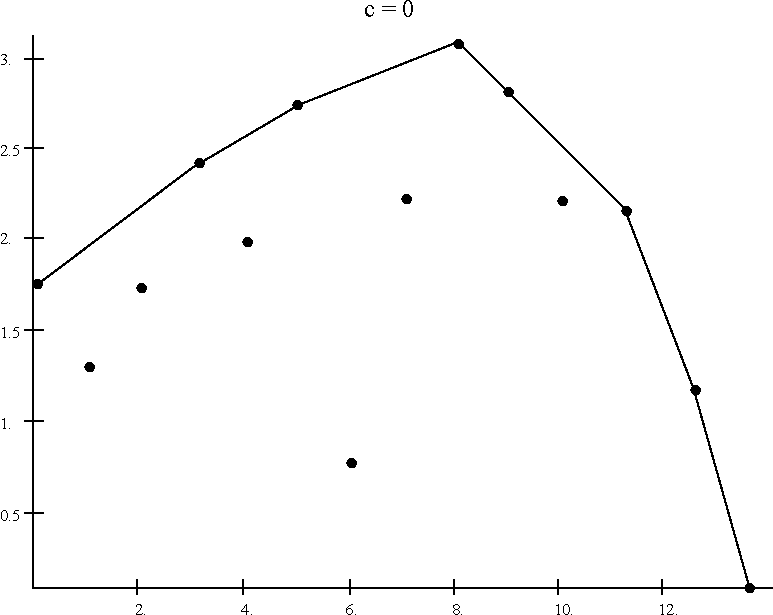
\includegraphics[width=\textwidth]{fig_1.pdf}
\caption{}
\label{fig:1}
\end{figure}

\begin{figure}
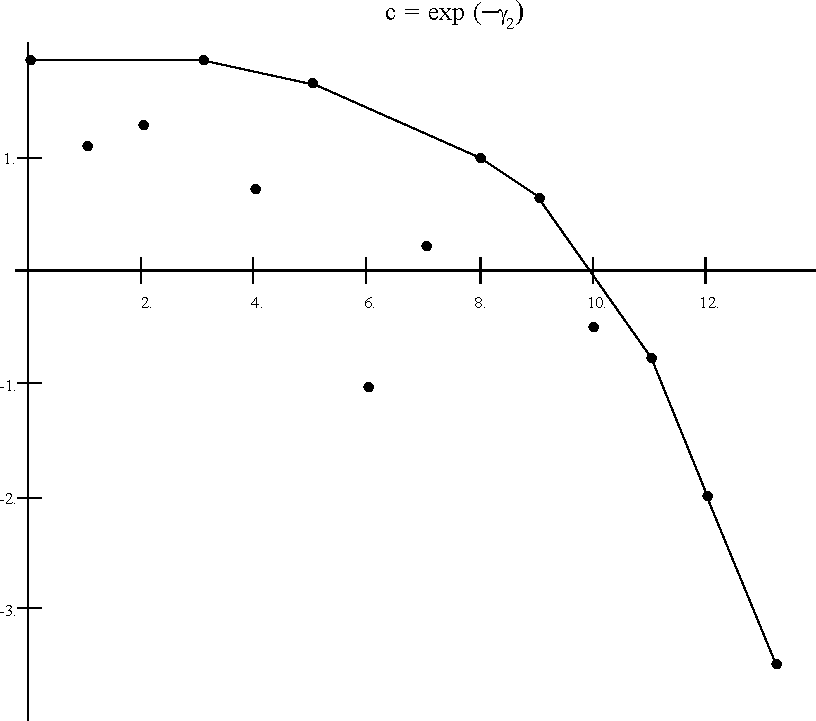
\includegraphics[width=\textwidth]{fig_2.pdf}
\caption{}
\label{fig:2}
\end{figure}

\begin{figure}
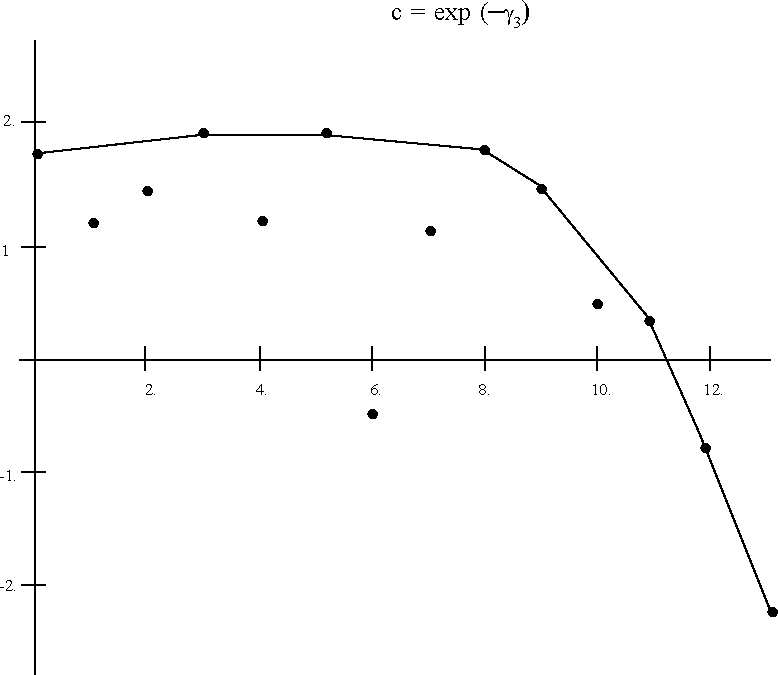
\includegraphics[width=\textwidth]{fig_3.pdf}
\caption{}
\label{fig:3}
\end{figure}

Now we would like to state the main result that we need concerning the Newton Polygon.

\begin{theo}[``Newton'']
\label{t3.2.3}
Let $K$ be complete, and let
$$
f(X)=a_{0}+a_{1}X+a_{2}X^{2}+\cdots+a_{n}X^{n}\in K[X]
$$
with $a_{0}\neq 0$ and $a_{n}\neq 0$. Suppose $N$ with $0<N<n$ such that
$$
\Vert a_{N}X^{N}\Vert=\Vert f\Vert\ ,
$$
\begin{center}
$\Vert a_{j}X^{j}\Vert<\Vert f\Vert$ for $j>N$
\end{center}
where $\Vert\, \cdot\, \Vert=\Vert\, \cdot\, \Vert_{C}$ for some $C$. Then there are $g,h\in K[X]$ with $\deg g=N$ and $\deg h=n-N$ and $f=gh$.
\end{theo}

The proof of this result is very much in the spirit of the proof of Hensel's Lemma.
\begin{proof}
The hypothesis implies that there is a $\Delta<1$ such that
$$
\left \Vert f(X)-\sum_{j=0}^{N}a_{j}X^{j}\right \Vert=\Delta\Vert f\Vert\ .
$$
We are now going to recursively define two sequences of polynomials, $g_{0},g_{1},\ldots$ and $h_{0},h_{1},\ldots$ which converge to $g$ and $h$ respectively. These sequences will satisfy the following conditions:
\begin{align*}
\deg g_{i}&=N\\
\deg h_{i}&\leq n-N,\\
\Vert f-g_{i}\Vert&\leq\Delta\Vert f\Vert\ ,\\
\Vert h_{i}-1\Vert&\leq\Delta\ .\\
\intertext{If we define $\delta_{i}$ by}
\Vert f-g_{i}h_{i}\Vert&=\delta_{i}\Vert f\Vert,
\end{align*}
then $\delta_{i}$ measures how far off $g_{i}h_{i}$ is from the true factorization $f=gh$. We want $\displaystyle \lim_{i\rightarrow\infty}\delta_{i}=0$. In any case our conditions on $g_{i}$ and $h_{i}$ tell us that $\delta_{i}\leq\Delta$. We will arrange it so that $\delta_{i+1}\leq\Delta\delta_{i}$, and since $\Delta<1$, this will insure convergence.

We get started with
$$
g_{0}(X)=\sum_{j=0}^{N}a_{j}X^{j},
$$
$$
h_{0}(X)=1\ .
$$

Thus we start with $\delta_{0}=\Delta$.

Now suppose we have $g_{i}$ and $h_{i}$, and we want $g_{i+1}$ and $h_{i+1}$. In order to conserve indexes, we write $G=g_{i}$ and $H=h_{i}$ and
$$
G(X)=b_{0}+b_{1}X+\cdots+b_{N}X^{N}\ .
$$
Since $\Vert f\Vert=\Vert a_{N}X^{N}\Vert$ and $\Vert f-G\Vert<\Vert f\Vert$, we must have $\Vert a_{N}X^{N}\Vert=\Vert b_{N}X^{N}\Vert$. Now if $\Vert b_{i}X^{i}\Vert>\Vert b_{N}X^{N}\Vert$, then we would have $\Vert f-G\Vert\geq\Vert(a_{i}-b_{i})X^{i}\Vert= \Vert b_{i}X^{i}\Vert>\Vert a_{N}X^{N}\Vert=\Vert f\Vert$ which is a contradiction. Hence we have $\Vert G\Vert= \Vert b_{N}X^{N}\Vert$.

Let $D=f-GH$ and divide $D$ by $G$ obtaining $Q,R\in K[X]$ with $D=QG+R$ and $\deg Q\leq n-N$ and $\deg R<N$.

\textbf{Claim.} $\Vert Q\Vert\leq\delta_{i}$ and $\Vert R\Vert\leq\delta_{i}\Vert f\Vert$.

We have $\Vert D\Vert=\delta_{i}\Vert f\Vert$ and $\Vert G\Vert=\Vert f\Vert$ so if we can prove $\Vert Q\Vert\cdot\Vert G\Vert\leq\Vert D\Vert$, the first part of the claim will follow. Let $c_{0},c_{1},\ldots,c_{n-N}$ be the coefficients of $Q$. They are determined by the linear equations
\begin{equation}
\label{eq3.35}
b_{N}c_{n-N-j}+b_{N-1^{C}n-N-j+1}+\cdots+b_{N-j^{C}n-N}=d_{n-j}
\end{equation}
where $d_{n-j}$ is the coefficient of $X^{n-j}$ in $D$, and $j$ runs from $0$ to $n-N$. We show
\begin{equation}
\label{eq3.36}
\Vert c_{n-N-j}X^{n-N-j}\Vert\cdot\Vert G\Vert\leq\Vert D\Vert
\end{equation}
by induction on $j$. For $j=0$, we get $b_{N}c_{n-N}=d_{n}$. Since we know that $\Vert G\Vert= C^{N}|b_{N}|$ and $\Vert D\Vert\geq C^{n}d_{n}$, the desired result follows (with equality) for $j=0$.

Now assume we know (\ref{eq3.36}) for $j-1$. Then we know that all of the terms in (\ref{eq3.35}) except for the first one have absolute value $\leq|d_{n-j}|$. If the $|b_{n}c_{n-N-j}|>|d_{n-j}|$, this would contradict the fact that the absolute value of the whole sum $=|d_{n-j}|$. Hence we get inequality (\ref{eq3.36}), and the first part of the claim follows.

The second part of the claim follows easily from the first part and the equation $D=QG+R$.

Now set $g_{i+1}=G+R(=g_{i}+R)$ and $h_{i+1}=H+Q(=h_{i}+Q)$. It is trivial to see that $g_{i+1}$ and $h_{i+1}$ satisfy the degree condition. The norm conditions follow from the claim, and it remains to show that $\delta_{i+1}\leq\Delta\delta_{i}$. We have
\begin{align*}
\delta_{i+1}\Vert f\Vert&=\Vert f-g_{i+1}h_{i+1}\Vert\\
&=\Vert f-(G+R)(H+Q)\Vert\\
&=\Vert(f-GH)-RH-QG-RQ\Vert\\
&=\Vert D-(D-R)-RH-RQ\Vert\\
&=\Vert R(H-1)+RQ\Vert\\
&\leq\max(\Vert R\Vert\cdot\Vert H-1\Vert,\Vert R\Vert\cdot\Vert Q\Vert)\\
&\leq\max(\Delta\delta_{i}\Vert f\Vert,\delta_{i}^{2}\Vert f\Vert)\\
&\leq\Delta\delta_{i}\Vert f\Vert
\end{align*}
as desired.
\end{proof}

\rem
In the factorization $f=gh$ we can assume (if we so desire) that $h(0)=1$ and that $\Vert h-1\Vert<1$ because we can replace $h$ by $[h(0)]^{-1}h$.

The form in which we use the theorem is the following:

\begin{coro}
\label{c3.2.5}
An irreducible polynomial in $K[X]$ is pure.
\end{coro}

\begin{proof}
Suppose $f$ is not pure. Let
$$
C=-\exp\left(\frac{1}{n}\ln\left|\frac{a_{n}}{a_{0}}\right|\right)\ .
$$
Picking this $C$ insures that $\Vert a_{0}\Vert=\Vert a_{n}X^{n}\Vert$, \ie, we can think of the line between $P_{0}$ and $P_{n}$ in the Newton Polygon $\Pi(f)$ as being horizontal. Since the slopes of the line segments in $\Pi(f)$ always decrease, we can find an index $N$ such that $P_{N}$ is the rightmost ``largest'' of the $P_{i}$'s. Then it is easy to see that with this $C$ and $N,f$ satisfies the hypothesis of the theorem, and so cannot be irreducible. 
\end{proof}

The next corollary is also sometimes referred to as ``Newton's Theorem''.

\begin{coro}
\label{c3.2.6}
Suppose that $K$ is complete and that $f\in K[x]$ is of type $(*)$, \ie, type $(\ell_{1},\gamma_{1};\ell_{2},\gamma_{2};\ldots;\ell_{r},\gamma_{r})$. Then $f$ factors
$$
f=g_{1}\cdot g_{2}\cdots g_{r}
$$
where $g_{s}$ is pure of type $(\ell_{s},\gamma_{s})$.
\end{coro}

\begin{proof}
Write $f=\Pi h_{\lambda}$ as a product of irreducible polynomials. By Corollary \ref{c3.2.5} each $h_{\lambda}$ is pure. If more than one of the $h_{\lambda}$'s have the same slope, then by Exercise \ref{e3.2.2} their product is pure with the same slope. Continuing in this fashion, we can write
$$
f=\prod_{\lambda=1}^{M}g_{\lambda}
$$
for some $M$, and say $g_{\lambda}$ is pure of type $(q_{\lambda},\delta_{\lambda})$ and $\delta_{1}>\delta_{2}>\cdots>\delta_{M}$. By Proposition \ref{p3.2.2} and a little induction, the type of $\Pi g_{\lambda}$ must be $(q_{1}, \delta_{1};q_{2},\delta_{2};\ldots ; q_{M},\delta_{M})$ which must be the type of $f$. Hence $M=r$ and $q_{i}=\ell_{i}$ and $\delta_{i}=\gamma_{i}$ for $1\leq i\leq r(=M)$.
\end{proof}

\rem
There is another corollary of our theorem which tells us that $f$ factors if we have a ``good enough'' approximate factorization. This says roughly that if $\delta=\Vert f-GH\Vert$ is less than $|R(G,H)|^{2}$ where $R(G,H)$ is the resultant of $G$ and $H$, then $f=gh$ where $\deg g=\deg G$ and $\deg h=\deg H$. For a proof see \cite{r2.4}, page 105.

\section{Extensions of Valuations}

Using the results of the previous section it is now relatively easy to show that we can extend a valuation (or absolute value) from a complete field to a finite extension.

\begin{theo}
\label{t3.3.4}Let $K$ be a field which is complete with respect to an absolute value $|\, \cdot\, |$, and let $L$ be an extension of $K$ of degree $n$. Define a map $\Vert\Vert:L\rightarrow \mathbb{R}$ by
$$
\Vert x\Vert=|N_{L/K}x|^{1/n}
$$
for $x\in L$. Then $\Vert\, \cdot\, \Vert$ is an absolute value on $L$ which extends $|\, \cdot\, |$.
\end{theo}

\begin{proof} If $x\in K$, then by Proposition \ref{p2.5.8} $\ N_{L/K}x=x^{n}$ so $\Vert x\Vert=|x|$ and $\Vert\, \cdot\, \Vert$ extends $|\, \cdot\, |$. Let $x, y\in L$. By Exercise \ref{e2.5.4} $N_{L/K}xy=N_{L/K}x\cdot N_{L/K}y$ so $\Vert xy\Vert=\Vert x\Vert\cdot\Vert y\Vert$. We now want to show that $\displaystyle \Vert x+y\Vert\leq\max(\Vert x\Vert,\Vert y\Vert)$. Suppose $\Vert y\Vert\leq\Vert x\Vert$. Then if $z=y/x$, we have $\Vert z\Vert\leq 1$, it suffices to show that $\Vert z+1\Vert\leq 1$. Let $f_{z}$ and $m_{z}$ be the characteristic and minimal polynomials of $z$ respectively. Then by Theorem \ref{t2.5.4} $f_{z}=m_{z}^{r}$ for some $r>0$. Write
$$
f_{z}(X)=X^{n}+a_{1}X^{n-1}+\cdots+a_{0}\ .
$$
Then $|a_{0}|=|\pm N_{L/K}z|\leq 1$ since $\Vert z\Vert\leq 1$. Now by Corollary \ref{c3.2.5}, since $m_{z}$ is irreducible, it is pure. By Exercise \ref{e3.2.2}, $f_{z}$ is thereby pure. Hence $|a_{i}|\leq|a_{0}|\leq 1$.

\begin{exo}
\label{e3.3.3}
Show that $N_{L/K}(1+z)=(-1)^{n}f_{z}(-1)$.
\end{exo}

Therefore
$$
\Vert 1+z\Vert=|f_{z}(-1)|^{1/n},
$$
and this is $\leq 1$ since the coefficients of $f_{z}$ have absolute value $\leq 1$.
\end{proof}
We can now show that this extension of a valuation on a complete field is unique, but the proof really has little to do with the preceding material. The idea is that a finite extension $L$ of $K$ is a finite dimensional vector space over $K$, and a finite dimensional vector space over a complete field has a unique topology. Instead of using topology directly, we introduce the familiar notion of a norm on a vector space.

\begin{defi}
\label{d3.3.2}
Let $V$ be a vector space over a field $K$ with valuation $|\, \cdot\, |$. A real valued function $\Vert\, \cdot\, \Vert$ on $V$ is called a {\it norm} if the following conditions hold $\forall\vec{a},\vec{b}\in V$ and $c\in K$:
\begin{enumerate}[(i)]
\item
$\Vert\vec{a}\Vert\geq 0$ and $\Vert\vec{a}\Vert=0$ if and only if $\vec{a}=0$.
\item
$\Vert\vec{a}+\vec{b}\Vert\leq\Vert\vec{a}\Vert+\Vert\vec{b}\Vert$.
\item
$\Vert c\vec{a}\Vert=|c|\cdot\Vert\vec{a}\Vert$.
\end{enumerate}
\end{defi}

\rems
\begin{enumerate}[(i)]
\item
This ``norm'' is, of course, different from the ``norm'' from an extension down to the base field, but this is the usual terminology. The context usually makes clear which one is intended.
\item
A norm on $V$ induces in the usual way a metric and thereby a topology on $V$. It should be clear that a norm on $V$ lets us define cauchy sequences of points of $V$, and hence what it means for $V$ to be complete.
\end{enumerate}

\begin{defi}
\label{d3.3.3}
Let $\Vert\, \cdot\, \Vert_{1}$ and $\Vert\, \cdot\, \Vert_{2}$ be norms on $V$. Then they are said to be {\it equivalent} if there are $C_{1},C_{2}\in \mathbb{R}$ such that $\Vert\vec{a}\Vert_{1}\leq C_{2}\Vert\vec{a}\Vert_{2}$ and $\Vert\vec{a}\Vert_{2}\leq C_{1}\Vert\vec{a}\Vert_{1}$.
\end{defi}

\rem
It can be shown that equivalent norms induce the same topology on $V$.

Here is the main result for this situation.

\begin{theo}
\label{t3.3.5}
Suppose $K$ is complete with respect to $|\, \cdot \, |$ and that $V$ is a finite dimensional vector space over $K$. Then any two norms extending  $|\, \cdot \, |$ on $V$ are equivalent, and $V$ is complete with respect to any such norm.
\end{theo}

\begin{proof}
Let $\vec{e}_{1},\vec{e}_{2},\ldots,\vec{e}_{n}$ be a basis for $V$ over $K$. For $\vec{a}\in K$ write
$$
\vec{a}=a_{1}\vec{e}_{1}+\cdots+a_{n}\vec{e}_{n}
$$
where $a_{i}\in K$. We define a canonical norm on $V$ by
$$
\Vert\vec{a}\Vert_{0}=\max_{i}|a_{i}|\ .
$$
It is easy to see that $\Vert\, \cdot\, \Vert_{0}$ is a norm and that $V$ is complete with respect to it. Hence it suffices to show that any norm on $V$ is equivalent to $\Vert\, \cdot\, \Vert_{0}$.

Let $\Vert\, \cdot\, \Vert$ be any norm on $V$. We must establish two inequalities. One is easy.
$$
\Vert a\Vert=\Vert\sum_{i}a_{i}\vec{e}_{i}\Vert
$$
$$
\leq\sum_{i}|a_{i}|\cdot\Vert\vec{e}_{i}\Vert
$$
$$
\leq C_{0}\Vert\vec{a}\Vert_{0}
$$
where
$$
 C_{0}=\sum_{i}\Vert\vec{e}_{i}\Vert\ .
$$
It remains to show that there is $C\in \mathbb{R}$ such that
\begin{equation}
\label{eq3.37}
\Vert\vec{a}\Vert_{0}\leq C \, \Vert a\Vert \quad \forall\vec{a}\in V .
\end{equation}
Suppose not. We derive a contradiction by induction on the dimension $n$ of $V$. Then $\forall \epsilon>0$ there is $\vec{b}=\vec{b}(\epsilon) \in V$ such that
$$
\Vert\vec{b}\Vert < \epsilon \, \Vert\vec{b}\Vert_{0}\ .
$$
By the definition of $\Vert\, \cdot\, \Vert_{0}$ we can assume that there is such a $\vec{b}$ with $\Vert\vec{b}\Vert_{0}=|b_{n}|$. (Permute the $\vec{e}_{i}$ if necessary.) Now replace $\vec{b}$ by $b_{n}^{-1}\cdot\vec{b}$ so $\vec{b}=\vec{c}+\vec{e}_{n}$ where $\vec{c}$ is in the subspace $W$ of $V$ spanned by $\vec{e}_{1},\ldots,\vec{e}_{n-1}$. In other words if (\ref{eq3.37}) is false, we can find a sequence $\{\vec{c}_{i}\}$ of elements of $W$ such that
$$
\lim_{i\rightarrow\infty}\Vert\vec{c}_{i}+\vec{e}_{n}\Vert=0\ .
$$
By the triangle inequality,
$$
\Vert(\vec{c}_{i}+\vec{e}_{n})-(\vec{c}_{j}+\vec{e}_{n})\Vert\leq\Vert\vec{c}_{i}+\vec{e}_{n}\Vert+\Vert\vec{c}_{j}+\vec{e}_{n}\Vert
$$
so
$$
\lim_{i, j\rightarrow\infty}\Vert\vec{c}_{i}-\vec{c}_{j}\Vert=0\ .
$$

Since the dimension of $W$ is less than the dimension of $V$, by induction we get $\vec{c}\in W$ such that
$$
\lim_{i\rightarrow\infty}\Vert\vec{c}_{i}-\vec{c}\Vert=0\ .
$$
This implies
$$
\Vert\vec{c}+\vec{e}_{n}\Vert=\lim_{i\rightarrow\infty}\Vert\vec{c}_{i}+\vec{e}_{n}\Vert=0\ .
$$
But $\vec{e}_{n}$ is certainly not in $W$ so $\vec{c}+\vec{e}_{n}\neq 0$ and we get our contradiction. Hence $\Vert\, \cdot\, \Vert_{0}$ and $\Vert\, \cdot\, \Vert$ are equivalent.
\end{proof}
Now we can easily prove the uniqueness of the extension of a valuation on a complete field.

\begin{coro}
\label{c3.3.7}
Let $K$ be a field which is complete with respect to an absolute value $|\, \cdot\, |$, and let $L$ be a finite extension of $K$. Then there is a unique extension of $|\, \cdot\, |$ to $L$, and $L$ is complete with respect to this extension.
\end{coro}

\begin{proof}
Theorem \ref{t3.3.4} tells us that there is an extension. If we regard $L$ as a finite dimensional vector space over $K$, then it is trivial to see that the extension of the absolute value defines a norm on $L$. If we had two extensions of the absolute value to $L$, then by the theorem they would be equivalent as norms on $L$.
\begin{exo}
\label{e3.3.4}
Show that any two equivalent norms on $L$ which agree on $K$ are identical.
\end{exo}

\begin{proof}
If $N_1$ and $N_2$ agree on $K$ which is complete. By theorem \ref{t3.3.5}, $N_1$ and $N_2$ are equivalent. Assume that there is $x\in L$ is s.t. $N_1(x)\neq N_2(x)$. Then, exchanging $N_1$ and $N_2$ if necessary, one has $N_1(x^n)/N_2(x^n)=\left[N_1(x)/N_2(x)\right]^n \to 0$ which contradicts the equivalence of the two norms. 

\end{proof}

The statement about the completeness of $L$ follows immediately from the completeness of the norm on $L$.
\end{proof}
We need one more trivial fact before we can prove the required result concerning extensions in the noncomplete case.
\begin{prop}
\label{p3.3.3}
Let $K$ be a complete field with respect to an absolute value. Then there is a unique extension of the absolute value to $\overline{K}$, the algebraic closure of $K$.
\end{prop}

\begin{proof}
Let $a\in\overline{K}$. We know that $a$ is algebraic over $K$ so the extension $K(a)$ is finite over $K$. By Corollary \ref{c3.3.7} the absolute value on $K$ extends uniquely to $K(a)$. For $a,b \in\overline{K}$ the extensions on $K(a)$ and $K(b)$ must also agree on $K(a)\cap K(b)$. These extensions therefore define a unique extension of the absolute value of $K$ to $\overline{K}$.
\end{proof}
We can now prove Theorem \ref{t2.8.12}. We restate it here in a slightly different form.

\begin{theo}
\label{t3.3.6}
Let $L=K(x)$ be a finite separable extension of $K$ and let $|\, \cdot\, |$ be an absolute value on $K$. Let $\overline{K}$ be the completion of $K$ with respect to $|\, \cdot\, |$. Let $m_{x}$ be the minimal polynomial of $x$. Suppose
$$
m_{x}=\varphi_{1}\varphi_{2}\cdots\varphi_{r}
$$
is the factorization of $m_{x}$ into (nonconstant) irreducibles in $\overline{K}[X]$.

Then the $\varphi_{i}$'s are distinct. Let $L_{i}=\overline{K}(y_{i})$ where $y_{i}$ is a root of $\varphi_{i}$. Then there is a monomorphism
$$
I_{i}\ :\ L=K(x)\mapsto L_{i}=\overline{K}(y_{i})
$$
which extends the monomorphism $K\mapsto\overline{K}$ under which $x\mapsto y_{i}$.  We know that the absolute value $|\, \cdot\, |$ extends uniquely to $\overline{K}$ and thence since $\overline{K}$ is complete, uniquely to $\overline{K}(y_{i})=L_{j}$. Using the monomorphism $I_{i}$, this defines an extension of $|\, \cdot\, |$ to $L$ which we denote by $|\, \cdot\, |_{i}$. Then the absolute values $|\, \cdot\, |_1, |\, \cdot\, |_2, \ldots, |\, \cdot\, |_{r}$ are precisely all of the extensions of $|\, \cdot\, |$ to $L$. Furthermore $L_{i}$ is the completion on $L$ with respect to $|\, \cdot\, |_{i}$.
\end{theo}

\begin{proof}
(As Cassels' remarks, the proof is shorter than the statement.) Let $\Vert\, \cdot\, \Vert$ be any extension of $|\, \cdot\, |$ to $L$, and let $\overline{L}$ be the completion of $L$ with respect to it. Then we have $\overline{K}\subset\overline{L}$ and $x\in L\subset\overline{L}$. By Corollary \ref{c3.3.7}, $\overline{K}(x)$ is complete so we must have $\overline{K}(x)$ isomorphic to $\overline{L}$ say by $I$. Clearly $I$ leaves $K$ fixed. Let $y=I(X)$, and let $m_{y}$ be the minimal polynomial for $y$ over $\overline{K}$. Since $m_{x}(x)=0$, and $I(m_{x})=m_{x}$ since $m_{x}\in K[X]$, we have $m_{x}(y)=0$ so $m_{y}|m_{x}$. Hence $m_{y}$ is one of the $\varphi_{i}$'s as desired.

Going in the other direction, let $y_{i}$ be a root of $\varphi_{i}$. Then $m_{x}(y_{i})=0$ so the extensions $K(x)=L$ and $k(y_{i})\subset\overline{k}(y_{i})=L_{i}$ are isomorphic, and we are reduced to the above situation.

It remains to show that the $\varphi_{i}$ are distinct. If not, $m_{x}$ and $m_{x}'$ would have a common factor in $\overline{K}[X]$. Now we can determine this common factor by the euclidean algorithm, so it must lie in $K[X]$, but this contradicts the fact that $m_{x}$ is irreducible and separable.
\end{proof}

\begin{thebibliography}{9}
\bibitem{r1.1} William Fulton. {\it Introduction to Intersection Theory in Algebraic Geometry}, number 54 in Regional Conference Series in Mathematics, American Mathematical Society, 1984.
\bibitem{r1.2} Serge Lang. {\it Algebra}, Addison-Wesley, 1965.
\bibitem{r1.3} Serge Lang. {\it Elliptic Curves}: {\it Diophantine Analysis}, Springer-Verlag, 1978.
\bibitem{r1.4} Chih-Han Sah. {\it Abstract Algebra}, Academic Press, 1967.
\bibitem{r1.5} Ren\'{e} Schoof. Elliptic curves over finite fields and the computation of square roots mod {\it p, Math. Comp}., 44:483-494, 1985.
\bibitem{r1.6} Joseph H. Silverman. {\it The Arithmetic of Elliptic Curves}, number 106 in Graduate Texts in Mathematics, Springer-Verlag, 1986.
\bibitem{r2.1} Emil Artin. Galois theory, {\it Notre Dame Mathematical Lectures}, 2, 1957.
\bibitem{r2.2} Emil Artin. {\it Algebraic Numbers and Algebraic Functions}, Nelson, London, 1968.
\bibitem{r2.3} Nicolas Bourbaki. {\it Commutative Algebra}, Hermann, Paris, 1972.
\bibitem{r2.4} J. W. S. Cassels. {\it Local Fields}, Cambridge Press, 1986.
%\bibitem{r2.5} Leonard S. Charlap and David P. Robbins. An elementary introduction to elliptic curves, CRD Expository Report No. 31, December 1988. IDA-CCR ${\rm Log}$ No. 82299.
\bibitem{r2.6} William Fulton. {\it Algebraic Curves}, W. A. Benjamin, 1969.
\bibitem{r2.7} Shigeru Iitaka. {\it Algebraic Geometry}, Springer-Verlag, 1982.
\bibitem{r2.8} Burt S. Kaliski. Elliptic curves and cryptography: A pseudorandom bit generator and other tools, MIT/LSC/TR-411, 1988. Cambridge.
\bibitem{r2.9} Keith Kendig. {\it Elementary Algebraic Geometry}, Springer-Verlag, 1977.
\bibitem{r2.11} Paul J. McCarthy. {\it Algebraic Extensions of Fields}, Blaisdell, 1966.
\bibitem{r2.13} Jean-Pierre Serre. {\it Groupes Alg\'{e}briques et Corps de Classes}, Hermann, 1959. Paris.
\bibitem{r2.14} Jean-Pierre Serre. {\it Local Fields}, Springer-Verlag, 1979.
\bibitem{r2.16} Edwin Weiss. {\it Algebraic Number Theory}, McGraw-Hill, 1963.
\bibitem{r2.17} Oscar Zariski and Pierre Samuel. {\it Commutative Algebra}, Van Nostrand, 1958.
\end{thebibliography}

\end{document}


